% !TEX program = xelatex
%% Compile with: xelatex main.tex && xelatex main.tex
%% (Run twice to resolve cross-references and table of contents.
%%  XeLaTeX is required for native Bengali (Bangla) script support via fontspec.)
%%
%% ============================================================
%%  KUET – CSE 4000: Thesis/Project – LaTeX Source
%%  Student  : [Student Name]      Roll : [Student ID]
%%  Title    : Bangla Word Sense Disambiguation: A Large-Scale Benchmark of Embedding and Classifier Combinations
%% ============================================================
\documentclass[12pt,a4paper]{report}

%                    
% PACKAGES
%                    
\usepackage{fontspec}
% Main body font: Times New Roman, matched to the reference template's
% mathptmx (Times) look. Requires XeLaTeX/LuaLaTeX (not pdflatex), since
% fontspec loads system fonts directly rather than TeX metrics.
\setmainfont{Times New Roman}
% Bengali (Bangla) script support: XeLaTeX + fontspec, via a dedicated
% Bengali-capable font wrapped in \bn{...}. 'Nirmala UI' ships with Windows
% 8+ and covers Bengali; if it is not found on your system, install the
% free 'Noto Sans Bengali' (Google Fonts) and change the font name below.
\newfontfamily\bengalifont[Script=Bengali]{Nirmala UI}
\newcommand{\bn}[1]{{\bengalifont #1}}
\usepackage[
  a4paper,
  top=1.2in,
  bottom=1.0in,
  left=1.2in,        % binding margin (template standard 1.2)
  right=1.0in,
  headheight=15pt,   % fancyhdr needs >=15pt for 12pt text
  headsep=14pt,
  footskip=0.4in     % footer 0.4 in from bottom edge
]{geometry}
\usepackage{setspace}
\usepackage{graphicx}
\usepackage{fancyhdr}
\usepackage{titlesec}
\usepackage{caption}
\usepackage{subcaption}
\usepackage{booktabs}
\usepackage{array}
\usepackage{tabularx}
\usepackage{multirow}
\usepackage{longtable}
\usepackage{enumitem}
\usepackage{ragged2e}
\usepackage[protrusion=true,expansion=false]{microtype}

%
% FLOAT PLACEMENT TUNING
%   Defaults (topfraction 0.7, floatpagefraction 0.5, etc.) let a figure
%   that only fills ~half a page get stranded alone on a mostly-blank
%   "float page" whenever several figures/tables cluster close together
%   in the source (e.g. Section 3.2's Table 3.1 / Figure 3.2 / Figure 3.3 /
%   Table 3.2 run). Raising these thresholds makes LaTeX try harder to
%   share a page between a float and body text before giving up and
%   dedicating a page to floats alone.
\renewcommand{\topfraction}{0.85}
\renewcommand{\bottomfraction}{0.85}
\renewcommand{\textfraction}{0.10}
\renewcommand{\floatpagefraction}{0.80}
\setlength{\floatsep}{10pt plus 2pt minus 2pt}
\setlength{\textfloatsep}{10pt plus 2pt minus 2pt}
\setlength{\intextsep}{10pt plus 2pt minus 2pt}

%
% HYPHENATION  (disabled globally, whole document)
%   No word is ever broken with an inserted line-end hyphen ("im-/plemented");
%   the whole word wraps to the next line instead. \hyphenpenalty=10000 makes
%   TeX treat *automatic* (soft) hyphenation as a forbidden line-break choice
%   (10000 is TeX's own "never" value); \lefthyphenmin/\righthyphenmin = 62
%   (TeX's maximum) is a redundant second safety net against automatic
%   hyphenation specifically. \exhyphenpenalty (breaking at a hyphen that is
%   already literally in the text, e.g. "BanglaBERT-FineTuned" in the narrow
%   result tables) is deliberately left at its default -- forbidding that too
%   caused new Overfull \hbox errors in those tables, and it is not the
%   mid-word breaking the user is asking to remove. Raising \tolerance and
%   \emergencystretch document-wide lets every line -- not just the body
%   paragraphs, which already set \sloppy\emergencystretch=3em locally --
%   absorb the resulting extra word-spacing so lines stay fully justified
%   (not ragged-right) without Overfull \hbox warnings. Margins, fonts,
%   sizes, line spacing, and indentation are untouched by these settings.
\tolerance=10000
\emergencystretch=3em
\hyphenpenalty=10000
\lefthyphenmin=62
\righthyphenmin=62

\usepackage[parfill]{parskip}  % suppress first-para indent globally
\usepackage{amsmath}
\usepackage{amssymb}
\usepackage{amsthm}
\usepackage{bm}
\usepackage{pifont}
\usepackage{chngcntr}           % continuous figure/table numbering
\usepackage{xcolor}
\usepackage{tikz}
\usetikzlibrary{shapes.geometric, arrows.meta, positioning, fit, backgrounds, calc}
\usepackage{pgfgantt}          % Gantt chart for the work-plan timeline
\usepackage{titletoc}           % TOC formatting (part of titlesec, compatible with hyperref)
\usepackage{hyperref}
\hypersetup{colorlinks=false, pdfborder={0 0 0}}

%                    
% NUMERIC NUMBERING FOR SECTIONS, FIGURES, TABLES
%                    
\renewcommand{\thesection}{\arabic{chapter}.\arabic{section}}
\renewcommand{\thefigure}{\arabic{chapter}.\arabic{figure}}
\renewcommand{\thetable}{\arabic{chapter}.\arabic{table}}
\renewcommand{\theequation}{\arabic{chapter}.\arabic{equation}}

%                    
% TOC DEPTH AND NUMBERING
%                    
\setcounter{tocdepth}{3}
\renewcommand{\thechapter}{\Roman{chapter}}

%                    
% GLOBAL SPACING
%   Body: 12 pt, 1.5 line spacing
%   Space before paragraph: 12 pt   Space after paragraph: 6 pt
%                    
\setstretch{1.5}
\setlength{\parindent}{0pt}
\setlength{\parskip}{12pt plus 2pt minus 2pt}
% Float-page spacing: by default LaTeX puts double stretch *between* floats
% on a floats-only page, which opens a large empty gap between stacked
% tables/figures. Pin floats to the top and push all slack to the bottom.
\makeatletter
\setlength{\@fptop}{0pt}
\setlength{\@fpsep}{14pt plus 2pt}
\setlength{\@fpbot}{0pt plus 1fil}
\makeatother

%                    
% HEADER / FOOTER
%   Header centred, 12 pt Normal
%   Footer: page number centred, 0.4 in from bottom edge
%                    
\pagestyle{fancy}
\fancyhf{}
\renewcommand{\headrulewidth}{0pt}
\renewcommand{\footrulewidth}{0pt}
% \fancyhead[C]{\fontsize{12}{14.4}\selectfont\normalfont CSE 4000: Thesis/Project}
\fancyfoot[C]{\thepage}

\fancypagestyle{plain}{
  \fancyhf{}
  \renewcommand{\headrulewidth}{0pt}
  \fancyfoot[C]{\thepage}
}

%                    
% CHAPTER FORMAT
%   "CHAPTER I"  : Times Roman, Bold, Centred, 14 pt, 1.5 spacing
%   [1 blank 12-pt line between label and title]
%   Chapter Title: Times Roman, Bold, Centred, 16 pt
%   [2 blank 12-pt lines (24 pt) after chapter title before body]
%                    
\titleformat{\chapter}[display]
  {\centering\bfseries\fontsize{14}{21}\selectfont}% label style
  {CHAPTER \thechapter}%                            label text
  {12pt}%                                           sep = 1 blank line
  {\centering\bfseries\fontsize{16}{24}\selectfont}% title style
\titlespacing*{\chapter}%
  {0pt}%   left indent
  {0pt}%   space above label
  {24pt}%  space after title (= 2 blank 12-pt lines)

%                    
% SECTION  :  Times Roman, Bold, Left-aligned, 14 pt, 1.5 spacing
%   Space before: 12 pt   Space after: 6 pt
%                    
\titleformat{\section}
  {\bfseries\fontsize{14}{21}\selectfont\raggedright}
  {\thesection}{1em}{}
\titlespacing*{\section}{0pt}{12pt}{6pt}

%                    
% SUBSECTION  :  Times Roman, Bold, Left-aligned, 12 pt, 1.5 spacing
%   Space before: 12 pt   Space after: 6 pt
%                    
\titleformat{\subsection}
  {\bfseries\fontsize{12}{18}\selectfont\raggedright}
  {\thesubsection}{1em}{}
\titlespacing*{\subsection}{0pt}{12pt}{6pt}

%                    
% SUBSUBSECTION  :  Times Roman, Bold, Left-aligned, 12 pt, 1.5 spacing
%   Space before: 12 pt   Space after: 6 pt
%                    
\titleformat{\subsubsection}
  {\bfseries\fontsize{12}{18}\selectfont\raggedright}
  {\thesubsubsection}{1em}{}
\titlespacing*{\subsubsection}{0pt}{12pt}{6pt}

%                    
% CAPTIONS  :  Times Roman, Normal, Centred, 11 pt, 1.5 spacing
%   Space before: 12 pt   Space after: 6 pt
%   Figure captions BELOW figure; Table captions ABOVE table
%                    
\DeclareCaptionFont{elevenpt}{\fontsize{11}{16.5}\selectfont}
\captionsetup{
  font={elevenpt,rm},
  labelfont=normalfont,
  textfont=normalfont,
  justification=centering,
  singlelinecheck=false,
  aboveskip=12pt,
  belowskip=6pt
}
\captionsetup[figure]{position=below}
\captionsetup[table]{position=above, aboveskip=0pt, belowskip=12pt}

%                    
% TOC / LOF / LOT FORMATTING  (via titletoc)
%   Times New Roman, Normal, 12 pt, 1.5 spacing
%   Chapter entries: no indent
%   Section entries: 0.5 in indent
%   Subsection entries: 1.0 in indent
%                    
\titlecontents{chapter}
  [0pt]                          % left margin
  {\addvspace{12pt}}             % above-code
  {\bfseries CHAPTER \thecontentslabel\quad}  % numbered entry format
  {\bfseries}   % unnumbered entry format (for front matter)
  {\hfill\contentspage}          % filler + page

\titlecontents{section}
  [0.5in]                        % 0.5 in indent
  {\normalfont}
  {\makebox[2.8em][l]{\thecontentslabel}}
  {}
  {\titlerule*[6pt]{.}\contentspage}

\titlecontents{subsection}
  [1.0in]                        % 1.0 in indent
  {\normalfont}
  {\makebox[3.6em][l]{\thecontentslabel}}
  {}
  {\titlerule*[6pt]{.}\contentspage}

\titlecontents{subsubsection}
  [1.5in]                        % 1.5 in indent
  {\normalfont}
  {\makebox[4.4em][l]{\thecontentslabel}}
  {}
  {\titlerule*[6pt]{.}\contentspage}

% Table/figure LOT/LOF entries use LaTeX's standard \@dottedtocline
% machinery: it glues the page number to the entry's last line inside the
% macro itself, so the number can never wrap onto its own line or collide
% with the description text. {0pt} = label column starts at the left
% margin; \WSDlotlabelw = label column width, and wrapped description
% lines hang at that same offset, aligned under the Description header.
% \WSDlistpagesetup (applied where the lists are typeset) right-aligns the
% page number in a \WSDlotpagew-wide box flush with the right margin --
% directly under the "Page" header -- and spaces the dot leaders out of
% existence so rows stay clean like the template's tabular layout.
\makeatletter
\newlength{\WSDlotlabelw}\setlength{\WSDlotlabelw}{0.8in}
\newlength{\WSDlotpagew}\setlength{\WSDlotpagew}{0.6in}
\renewcommand*{\l@table}{\@dottedtocline{1}{0pt}{\WSDlotlabelw}}
\renewcommand*{\l@figure}{\@dottedtocline{1}{0pt}{\WSDlotlabelw}}
\newcommand{\WSDlistpagesetup}{%
  \renewcommand{\@pnumwidth}{\WSDlotpagew}%
  \renewcommand{\@tocrmarg}{0.8in}%
  \renewcommand{\@dotsep}{10000}%
}
\makeatother

%                    
% BIBLIOGRAPHY FORMATTING  (IEEE standard)
%   12 pt, Normal, Justified, 1.2 line spacing
%   Space before & after entry: 6 pt
%   Left indent: 0 in   Hanging indent: 0.31 in
%                    
\let\oldbibliography\thebibliography
\renewcommand{\thebibliography}[1]{%
  \oldbibliography{#1}%
  \setstretch{1.2}%
  \setlength{\parskip}{6pt}%
  \setlength{\itemsep}{6pt}%
  \setlength{\leftmargin}{0pt}%
  \setlength{\labelsep}{0.31in}%
}

%                    
% SPACING HELPERS
%   One "blank line" at body size (12 pt) = 18 pt (line spacing 1.5)
%   Template specifies blank lines in 12 pt units:
%     1 blank line  = 18 pt (1.5 × 12)
%     2 blank lines = 36 pt
%     3 blank lines = 54 pt
%                    
\newcommand{\oneblank}{\vspace{18pt}}
\newcommand{\twoblank}{\vspace{36pt}}
\newcommand{\threeblank}{\vspace{54pt}}
\newcommand{\fourblank}{\vspace{72pt}}

%                    
% KUET LOGO COMMAND
%   Includes kuet_logo.{png,jpg,pdf} if it exists on disk;
%   otherwise draws a labelled placeholder box of the same
%   1.14" x 1.0" dimensions so the document always compiles.
%                    
\newcommand{\kuetlogo}{%
  \IfFileExists{kuet_logo.pdf}{%
    
\includegraphics[width=1.14in,height=1.0in,keepaspectratio=false]{kuet_logo}%
  }
}

%============================================================
\begin{document}
%============================================================

%============================================================
%  COVER PAGE  (no header, no footer, no page number)
%  Template: Title 18pt Bold Small Caps centred; "By" 14pt;
%  2 blank lines before "By"; 3 blank lines after "By";
%  KUET logo 1.14" x 1.0"; Dept info 12pt Bold 1.2 spacing
%  pushed to bottom 1.0" from edge via \vfill.
%============================================================
\thispagestyle{empty}

\begin{center}

\makebox[\textwidth][l]{\raisebox{0.5in}[0pt][0pt]{Project/Thesis No: CSER-26-06}}\\[-\baselineskip]
{\fontsize{14}{21}\selectfont\bfseries
CSE 4000: Thesis/Project}

\vspace{6pt}

% Thesis Title: 18 pt, Bold, Centred, Small Caps, 1.5 spacing  
{\fontsize{18}{27}\selectfont\bfseries\scshape Bangla Word Sense Disambiguation: A Large-Scale Benchmark of Embedding and Classifier Combinations}

%  2 blank lines (12 pt each) between title and "By"  
\twoblank

%  "By": 14 pt, Normal, Centred  
{\fontsize{14}{21}\selectfont\normalfont By}

%  3 blank lines below "By"  
\threeblank

%  Student Name: 14 pt, Bold; Roll: 14 pt, Normal  
{\fontsize{14}{21}\selectfont\bfseries Prova Rani Paul}\\[6pt]
{\fontsize{14}{21}\selectfont\normalfont Roll: 2007037}

\vfill

%  KUET Logo: exactly 1.14" wide × 1.0" tall  

\includegraphics[width=1.14in]{kuet_logo}
\vfill

\end{center}

%  Bottom dept info: 12 pt, Bold, Centred, 1.2 spacing  
%  Pushed to very bottom (1.0" from edge) by preceding \vfill  
{\setstretch{1.2}%
\begin{center}
{\fontsize{12}{14.4}\selectfont\bfseries
Department of Computer Science and Engineering\\
Khulna University of Engineering \& Technology\\
Khulna 9203, Bangladesh\\
July, 2026}
\end{center}}

%============================================================
%  FRONT MATTER  –  Roman numerals
%============================================================
\newpage
\pagenumbering{roman}
\setcounter{page}{1}

%============================================================
%  TITLE PAGE  (page i)
%============================================================
\thispagestyle{plain}
% Inject "PAGE" at the very top of the TOC
\addtocontents{toc}{\protect\hfill\textbf{PAGE}\par\vspace{6pt}}
\addcontentsline{toc}{chapter}{Title Page}

%  Title Page  
%   Title: 18 pt, Bold, Centred, 1.5 spacing
\begin{center}
{\fontsize{18}{27}\selectfont\bfseries Bangla Word Sense Disambiguation: A Large-Scale Benchmark of Embedding and Classifier Combinations}
\end{center}

%  3 blank lines between title and "By"  
\threeblank

%  "By": 12 pt, Normal, Centred  
\begin{center}
{\fontsize{12}{18}\selectfont\normalfont By}
\end{center}

%  2 blank lines below "By"  
\twoblank

%  Student Name: 12 pt, Bold; Roll: 12 pt, Normal  
\begin{center}
{\fontsize{12}{18}\selectfont\bfseries Prova Rani Paul}\\[6pt]
{\fontsize{12}{18}\selectfont\normalfont Roll: 2007037}
\end{center}

\vspace{36pt}

\begin{center}
{\fontsize{12}{18}\selectfont\normalfont
A thesis submitted in partial fulfillment of the requirements for the degree of\\[6pt]
``Bachelor of Science in Computer Science \& Engineering''
}
\end{center}

\vspace{36pt}

%  Supervisor section  
%   "Supervisor:": 12 pt, Bold, left-aligned
\noindent{\fontsize{12}{18}\selectfont\bfseries Supervisor:}

\vspace{6pt}

%   Name, Designation, Dept: 12 pt, 0.8" left indent
\noindent\hspace*{0.8in}%
\begin{tabular}{@{} >{\raggedright\arraybackslash}p{3.4in} >{\centering\arraybackslash}p{1.2in}@{}}

{\fontsize{12}{18}\selectfont\bfseries Dr. K. M. Azharul Hasan} & \\[6pt]

{\fontsize{12}{18}\selectfont\normalfont Professor} & \\[6pt]

{\fontsize{12}{18}\selectfont\normalfont Department of Computer Science and Engineering} &
\rule{1.2in}{0.4pt} \\[2pt]

{\fontsize{12}{18}\selectfont\normalfont Khulna University of Engineering \& Technology} &
{\fontsize{12}{18}\selectfont\normalfont Signature} \\

\end{tabular}
\vfill

%  Bottom: Dept info 12 pt, Normal, Centred; Date 16 pt, Bold, Centred  
\begin{center}
{\fontsize{12}{18}\selectfont\normalfont
Department of Computer Science and Engineering\\
Khulna University of Engineering \& Technology\\
Khulna 9203, Bangladesh\\
July, 2026}
\end{center}

%============================================================
%  ACKNOWLEDGMENT  (page ii)
%============================================================
\newpage
\thispagestyle{plain}
\addcontentsline{toc}{chapter}{Acknowledgment}

\begin{center}
{\fontsize{16}{24}\selectfont\bfseries Acknowledgment}
\end{center}

\twoblank

{\fontsize{12}{18}\selectfont\normalfont\setstretch{1.5}
\justifying\sloppy\emergencystretch=3em
First and foremost, all praises to the Almighty for His countless blessings and guidance. I would like to express my sincere gratitude to Dr. K. M. Azharul Hasan, Professor, Department of Computer Science and Engineering, Khulna University of Engineering \& Technology, for expert supervision, constructive guidance, and consistent encouragement throughout the course of this research. Appreciation is also extended to the faculty members and staff of the Department of Computer Science and Engineering for their academic support, to the two annotators whose careful labelling effort made the corpus underlying this thesis possible, and to family and friends for their enduring encouragement, without whose support this work would not have been possible.
}

\begin{flushright}
{\fontsize{12}{18}\selectfont\bfseries Author}
\end{flushright}

%============================================================
%  ABSTRACT  (page iii)
%============================================================
\newpage
\thispagestyle{plain}
\addcontentsline{toc}{chapter}{Abstract}

\begin{center}
{\fontsize{16}{24}\selectfont\bfseries Abstract}
\end{center}

\twoblank

{\fontsize{12}{18}\selectfont\normalfont\setstretch{1.5}
\justifying\sloppy\emergencystretch=3em
Word Sense Disambiguation (WSD) is the task of automatically selecting the correct meaning of an ambiguous word from a predefined sense inventory, given the context in which it occurs. Bangla, despite being spoken natively by more than 230 million people, has no large-scale, publicly verifiable, reliability-checked sense-tagged corpus, and no prior published study has benchmarked classical machine learning, sequence deep learning, and transformer fine-tuning for this task under one shared experimental protocol. This thesis addresses both gaps. A purpose-built, web-based annotation platform (PHP and MySQL) was developed through which two independent annotators labelled 7,409 Bangla sentences spanning 181 polysemous target words; inter-annotator reliability was quantified using Cohen's Kappa (\(\kappa = 0.836\) and \(\kappa = 0.874\), both in the \emph{almost perfect} agreement band). After preprocessing and a word-specific label re-engineering that eliminates cross-word sense-identifier collision, 7,381 sentences across 657 unique classes and 179 target words remained. A controlled, twenty-nine-experiment benchmark was then conducted on one fixed stratified 70/15/15 split, comparing six text representations (TF--IDF and pretrained Word2Vec, fastText, multilingual BERT, BanglaBERT, and XLM-RoBERTa embeddings) against three classical learners (Naive Bayes, Logistic Regression, Linear SVM) on every representation and four recurrent architectures (LSTM, GRU, BiLSTM, BiGRU) on the two sequence-capable representations, together with three fully fine-tuned transformer models, every configuration scored under one shared metric suite in both a global 657-way setting and a target-word-constrained inference setting. Fine-tuned BanglaBERT achieved the best result, 86.82\% accuracy and 85.00\% macro F1, outperforming fine-tuned multilingual BERT by 7.2 macro-F1 points, while frozen XLM-RoBERTa embeddings paired with simple logistic regression reached 86.37\% accuracy at a small fraction of the training cost; fine-tuning XLM-RoBERTa itself under the identical recipe failed to converge, a negative result reported and analysed rather than concealed. The two strongest fine-tuned models were deployed in an interactive Gradio web application for real-time Bangla sense disambiguation. This thesis thereby contributes a reusable, human-validated Bangla WSD resource and, so far as the reviewed literature shows, the first systematic comparison of classical, deep-learning, and transformer-based approaches to Bangla word sense disambiguation reported under a single, controlled experimental protocol.
}

%============================================================
%  TABLE OF CONTENTS  –  auto-generated
%============================================================
\newpage
\thispagestyle{plain}
\addcontentsline{toc}{chapter}{Contents}
{\setstretch{1.5}
\tableofcontents
}

%============================================================
%  LIST OF TABLES
%============================================================
\newpage
\thispagestyle{plain}
\addcontentsline{toc}{chapter}{List of Tables}

\addtocontents{lot}{%
\noindent
\makebox[\WSDlotlabelw][l]{\textbf{Table No.}}%
\makebox[\dimexpr\linewidth-\WSDlotlabelw-\WSDlotpagew\relax][c]{\textbf{Description}}%
\makebox[\WSDlotpagew][r]{\textbf{Page}}%
\par\vspace{12pt}%
}

{\setstretch{1.5}\sloppy\WSDlistpagesetup
\listoftables
}

%============================================================
%  LIST OF FIGURES
%============================================================
\newpage
\thispagestyle{plain}
\addcontentsline{toc}{chapter}{List of Figures}

\addtocontents{lof}{%
\noindent
\makebox[\WSDlotlabelw][l]{\textbf{Figure No.}}%
\makebox[\dimexpr\linewidth-\WSDlotlabelw-\WSDlotpagew\relax][c]{\textbf{Description}}%
\makebox[\WSDlotpagew][r]{\textbf{Page}}%
\par\vspace{12pt}%
}

{\setstretch{1.5}\sloppy\WSDlistpagesetup
\listoffigures
}

%============================================================
%  MAIN MATTER  –  Arabic numerals
%============================================================
\newpage
\pagenumbering{arabic}
\setcounter{page}{1}

%============================================================
%  CHAPTER I  –  Introduction
%============================================================
\chapter{Introduction}

\section{Introduction}
{\fontsize{12}{18}\selectfont\normalfont\setstretch{1.5}\justifying\sloppy\emergencystretch=3em
Natural Language Processing (NLP) enables machines to read, interpret, and reason about human language, but natural languages are inherently ambiguous at the lexical level: a single word form can carry multiple, often unrelated, meanings depending on context. This is called lexical ambiguity, and Word Sense Disambiguation (WSD) is the task of automatically selecting the correct sense of an ambiguous word from a predefined inventory of candidate senses, given the sentence it occurs in \cite{ide1998wsd}, \cite{navigli2009wsd}. WSD underlies machine translation, search, question answering, and sentiment analysis, and for English it has been studied for decades using shared benchmarks such as Senseval and SemEval.\par

Bangla (Bengali), spoken natively by more than 230 million people, has received far less attention. It is morphologically rich (a single verb root may take over one hundred inflected forms), permits flexible word order, and is documented to exhibit unusually high polysemy: the target word \bn{জল} alone is annotated in the corpus built for this thesis with at least three unrelated senses ("exhausting labour", "tears", and "rain"), each distinguishable only by context. No large, standardized, sense-tagged Bangla corpus exists in the way SemCor or Princeton WordNet exist for English, and pretrained Bangla embeddings have only recently become available, which together make Bangla WSD both harder and less studied than its English counterpart.\par

Prior Bangla WSD research (reviewed critically in Chapter 2) relies on small, private corpora and hand-engineered features; none benchmarks modern embeddings or transformer fine-tuning, and none reports a quantified inter-annotator reliability check. This thesis takes on both gaps. A custom web annotation platform was used to label 7,409 Bangla sentences across 181 target words, with reliability quantified via Cohen's Kappa. A controlled, twenty-nine-experiment benchmark then compares six text representations (TF-IDF and pretrained Word2Vec, fastText, and mBERT \cite{devlin2019bert}, BanglaBERT \cite{bhattacharjee2022banglabert}, XLM-RoBERTa \cite{conneau2020xlmr} embeddings) against three classical learners, four recurrent architectures, and three fully fine-tuned transformers, all under one fixed stratified split and one shared metric suite, with the best models deployed in a live web demo.\par

}
\section{Problem Statement}
{\fontsize{12}{18}\selectfont\normalfont\setstretch{1.5}\justifying\sloppy\emergencystretch=3em
Three interlocking deficiencies motivate this thesis. First, dataset scarcity: Bangla has no large, publicly verifiable, sense-tagged benchmark corpus; existing datasets span only 7-100 target words (Pal \& Saha: 7 words/2,478 sentences; Nazah et al.: 50 words/160 sentences; Saha et al.: 100 words/3,860 sentences; Das Dawn et al.: 100 words, public but small), so every study evaluates against a dataset of its own making. Second, annotation reliability: no prior Bangla WSD study reports a Cohen's Kappa or comparable statistic, despite labels usually being assigned by the researchers themselves. Third, methodological narrowness: prior work relies exclusively on hand-engineered features (edit distance, cosine similarity, Naive Bayes) and never benchmarks learned embeddings, sequence deep learning, or transformer fine-tuning under shared conditions.\par

A further problem, cross-word label collision, arises directly from the source data: the raw sense\_id (1-4) is reused across unrelated words, so \bn{বর্ণ} ("colour") and \bn{হাত} ("body part") can share sense\_id = 1, forcing a shared classifier to learn contradictory labels. Correcting this by re-keying each label to (target\_word + sense\_gloss) is a necessary precondition for training a single classifier across all 179 words. Together these four deficiencies (no benchmark, no reliability check, no representation-learning comparison, and label collision) define the problem this thesis solves.\par

}
\section{Objectives}
{\fontsize{12}{18}\selectfont\normalfont\setstretch{1.5}\justifying\sloppy\emergencystretch=3em
The objectives pursued and achieved in this thesis are:\par

\begin{enumerate}[leftmargin=*, itemsep=4pt]
  \item Design and implement a web-based annotation platform (PHP/MySQL) supporting dataset import, randomized-order sense presentation, and per-annotator submission tracking.
  \item Build a human-annotated Bangla WSD corpus (7,409 sentences, 181 target words, 637 sense glosses) and quantify annotation reliability via Cohen's Kappa.
  \item Re-engineer the label space as target\_word + sense\_gloss so that cross-word collision disappears, giving 657 unique classes across 179 words.
  \item Benchmark six embeddings (TF-IDF and pretrained Word2Vec, fastText, mBERT, BanglaBERT, XLM-R) against three classical learners (Naive Bayes, Logistic Regression, Linear SVM), and the two sequence-capable embeddings (Word2Vec, fastText) against four recurrent architectures (LSTM, GRU, BiLSTM, BiGRU), on one fixed stratified split.
  \item Fine-tune mBERT, BanglaBERT, and XLM-R end-to-end with an identical recipe on the same fixed split.
  \item Evaluate all twenty-nine configurations with a shared metric suite (accuracy, macro/weighted P/R/F1, balanced accuracy, MCC, Cohen's Kappa, ROC-AUC, timing, and memory footprint), under both global and target-word-constrained inference.
  \item Analyse confusion-matrix errors of the best models and relate them to class imbalance and semantic proximity between senses.
  \item Deploy the two most accurate fine-tuned models in an interactive Gradio application with sense-restricted prediction and live benchmark comparison.
\end{enumerate}
}
\section{Scope}
{\fontsize{12}{18}\selectfont\normalfont\setstretch{1.5}\justifying\sloppy\emergencystretch=3em
The scope is bounded so the benchmark remains controlled and reproducible. Dataset: 181 target words, target-word (lexical-sample) formulation, not all-words WSD; after preprocessing, 7,381 sentences across 657 classes and 179 words remain. Preprocessing is limited to null/duplicate removal, target-word verification, and word-specific label construction; no stemming, POS tagging, or parsing is performed. Exactly six embedding families are used (TF-IDF, pretrained Word2Vec and fastText, and frozen mBERT/BanglaBERT/XLM-R target-span embeddings); others (GloVe, Sentence-BERT) are out of scope. Three classical learners sit on top of all six embeddings (eighteen experiments), four sequence architectures sit on top of the two embeddings with genuine per-token structure (eight experiments), and three transformers are fully fine-tuned (three experiments), twenty-nine experiments in total. Metrics form a shared suite computed on a held-out test split, reported both globally over all 657 classes and under target-word-constrained inference. Fine-tuning means full end-to-end updates of a pretrained encoder; parameter-efficient methods (LoRA, adapters) are not evaluated.\par

Three limitations are acknowledged as part of this scope. All twenty-nine experiments share a single fixed stratified split (seed 42) rather than being repeated across multiple splits, because of the computational cost of repeating transformer fine-tuning; the split indices are persisted so the exact partition is reproducible and auditable. XLM-R fine-tuning fails to converge under the shared recipe; Section 4.5 reports and analyses this negative result. The fitted TF-IDF/Word2Vec/fastText artefacts were not exported, so only fine-tuned transformers are runnable in the live demo. The label space, platform, and pipeline are nonetheless designed to be extended with additional words, embeddings, or models without redesign.\par

}
\section{Financial Analysis}
{\fontsize{12}{18}\selectfont\normalfont\setstretch{1.5}\justifying\sloppy\emergencystretch=3em
This research used almost entirely free and open-source software and free-tier cloud compute, keeping direct monetary cost low. Table 1.1 itemises the estimated resource cost in Bangladeshi Taka (BDT).\par

}
\begin{table}[htbp]
\caption{Estimated project resource and cost breakdown.}
\label{tab:auto1}
\centering
{\fontsize{10}{14}\selectfont
\begin{tabular}{@{}p{2.60cm} p{3.75cm} p{3.75cm} p{3.75cm}@{}}
\toprule
\textbf{Category} & \textbf{Item} & \textbf{Est. Cost (BDT)} & \textbf{Remarks} \\
\midrule
Hardware & Laptop/desktop (amortised), internet, electricity & 16,000 & \textasciitilde{}8 months \\
\addlinespace[3pt]
Cloud Compute & GPU training (Kaggle free-tier Tesla T4) & 0 & 29 experiments incl.\ transformer fine-tuning \\
\addlinespace[3pt]
Software & Python, PyTorch, HuggingFace, PHP, MySQL, Gradio & 0 & Open-source \\
\addlinespace[3pt]
Human Resources & Annotator honorarium (2 annotators) & 6,000 & Token compensation \\
\addlinespace[3pt]
Reporting & Printing, binding, presentation materials & 2,000 & Draft and final copies \\
\addlinespace[3pt]
Total &  & 24,000 & All values in BDT; direct out-of-pocket cost \\
\addlinespace[3pt]
\bottomrule
\end{tabular}}
\end{table}
{\fontsize{12}{18}\selectfont\normalfont\setstretch{1.5}\justifying\sloppy\emergencystretch=3em
The total, approximately 24,000 BDT, is dominated by connectivity, electricity, and the annotator honorarium; model-training compute was obtained free via Kaggle's GPU tier, avoiding what would otherwise be a non-trivial cloud budget for the transformer fine-tuning stage.\par

}
\section{Unfamiliarity of the Problem}
{\fontsize{12}{18}\selectfont\normalfont\setstretch{1.5}\justifying\sloppy\emergencystretch=3em
No prior published Bangla WSD study combines a custom annotation platform, a quantified reliability check, a collision-free label space, and a benchmark spanning classical ML through transformer fine-tuning. Each part is individually well-established, but no existing codebase integrated them for Bangla, so interfaces such as the raw-sense\_id-to-collision-free-label mapping, the shared [TGT] marker logic reused between training and live inference, and the automatic model-selection logic in the deployed demo each required original engineering rather than routine application of a known recipe. This was compounded by the absence of comparable prior results: when XLM-R fine-tuning failed to converge under the recipe that worked for mBERT and BanglaBERT, there was no prior Bangla result to indicate whether this was a bug or a genuine backbone-specific phenomenon, so the failure had to be investigated independently, verifying the tokenizer's handling of the [TGT] markers, the label mapping, and the gradient flow each in isolation, with no known outcome to replicate.\par

}
\section{Project Planning and Work Distribution}
{\fontsize{12}{18}\selectfont\normalfont\setstretch{1.5}\justifying\sloppy\emergencystretch=3em
The thesis was completed by a single candidate over roughly twenty-four to twenty-six weeks. Figure~\ref{fig:timeline} presents the preliminary work-plan timeline; annotation-platform development and corpus annotation were deliberately overlapped, while the transformer fine-tuning stage was scheduled only after the shared preprocessing and classical/sequence benchmark pipeline was validated as stable, since transformer fine-tuning is by far the most computationally expensive stage.\par

}
\begin{figure}[htbp]
\centering
\resizebox{\textwidth}{!}{%
\begin{ganttchart}[
    vgrid,
    hgrid,
    title height=1,
    bar height=0.6,
    bar label font=\small,
    title label font=\small\bfseries,
    bar/.append style={rounded corners=1pt},
    y unit title=0.75cm,
    y unit chart=0.75cm,
    x unit=0.55cm
  ]{1}{26}
  \gantttitle{1st Term}{13}
  \gantttitle{2nd Term}{13} \\
  \gantttitlelist{1,...,13}{1}\gantttitlelist{1,...,13}{1} \\
  \ganttbar[bar/.append style={fill=violet}]{Topic Selection}{1}{2} \\
  \ganttbar[bar/.append style={fill=blue!70}]{Topic Confirmation}{2}{3} \\
  \ganttbar[bar/.append style={fill=magenta}]{Literature Review}{3}{6} \\
  \ganttbar[bar/.append style={fill=cyan!80!black}]{Annotation Platform Design}{4}{5} \\
  \ganttbar[bar/.append style={fill=blue}]{Annotation Platform Development}{5}{7} \\
  \ganttbar[bar/.append style={fill=green!60!black}]{Dataset Annotation}{6}{11} \\
  \ganttbar[bar/.append style={fill=teal}]{Cohen's Kappa Validation}{10}{12} \\
  \ganttbar[bar/.append style={fill=brown}]{Preprocessing \& Label Engineering}{11}{13} \\
  \ganttbar[bar/.append style={fill=olive}]{Embedding Generation}{12}{14} \\
  \ganttbar[bar/.append style={fill=gray}]{Classical/Sequence Benchmark}{14}{18} \\
  \ganttbar[bar/.append style={fill=orange}]{Transformer Fine-tuning}{17}{21} \\
  \ganttbar[bar/.append style={fill=red}]{Error Analysis}{20}{22} \\
  \ganttbar[bar/.append style={fill=pink}]{Demo Deployment}{21}{23} \\
  \ganttbar[bar/.append style={fill=purple}]{Result Synthesis}{22}{23} \\
  \ganttbar[bar/.append style={fill=violet!60}]{Thesis Writing}{18}{25} \\
  \ganttbar[bar/.append style={fill=red!70!black}]{Defence Preparation}{24}{26} \\
\end{ganttchart}%
}
\caption{Gantt chart of the thesis work plan.}
\label{fig:timeline}
\end{figure}
\section{Contributions}
{\fontsize{12}{18}\selectfont\normalfont\setstretch{1.5}\justifying\sloppy\emergencystretch=3em
The principal original contributions of this thesis are:\par

\begin{enumerate}[leftmargin=*, itemsep=4pt]
  \item A purpose-built PHP/MySQL annotation platform with deduplication, randomized-order sense presentation, and an integrated Cohen's Kappa dashboard.
  \item A human-validated Bangla WSD corpus of 7,409 sentences across 181 target words, with reliability quantified at \(\kappa = 0.836\) and \(0.874\) ("almost perfect" per Landis and Koch \cite{landis1977kappa}), larger by target-word count than every prior Bangla WSD dataset reviewed.
  \item A word-specific label re-engineering (target\_word + sense\_gloss) producing 657 non-colliding classes trained as one global classification problem.
  \item A controlled twenty-nine-experiment benchmark spanning classical ML, sequence deep learning, and transformer fine-tuning under one shared split and metric suite, with every configuration additionally evaluated under target-word-constrained inference; no prior Bangla WSD study reviewed in Chapter 2 reports such a comparison.
  \item Empirical evidence that Bangla-specific pretraining matters: fine-tuned BanglaBERT reaches 86.82\% accuracy / 85.00\% macro F1, outperforming fine-tuned mBERT by 7.2 macro-F1 points, while frozen XLM-R target-span embeddings with plain logistic regression come within half an accuracy point of the best fine-tuned model at a small fraction of its training cost.
  \item A documented negative result: XLM-R fine-tuning fails to converge (0.09\% accuracy) under the identical recipe that succeeds for mBERT and BanglaBERT, even after the [TGT] markers are registered as atomic special tokens and label mapping and gradient flow are verified; Section 4.5 analyses this failure in detail.
  \item A deployable Gradio application that auto-selects the two most accurate fine-tuned models from the benchmark table and applies sense-restricted prediction.
\end{enumerate}
}
\section{Applications}
{\fontsize{12}{18}\selectfont\normalfont\setstretch{1.5}\justifying\sloppy\emergencystretch=3em
Beyond benchmarking, the corpus, platform, and trained models have direct applications:\par

\begin{enumerate}[leftmargin=*, itemsep=4pt]
  \item Machine Translation: disambiguating a source word's sense before selecting its target-language equivalent.
  \item Information Retrieval: disambiguating query and document terms to reduce retrieval of documents sharing only a word form, not its intended meaning.
  \item Question Answering and Conversational Agents: resolving ambiguous words in user queries before answer retrieval, e.g. in agriculture or health chatbots.
  \item Sentiment Analysis: several annotated words (e.g. \bn{রূপ}, "shape" vs. "beauty") carry senses with opposite affective connotations, so sense resolution can reduce polarity error.
  \item Education: the sense-tagged corpus with authentic example sentences can serve as Bangla vocabulary teaching material.
  \item Spell/Usage Correction: flagging a word used in a context inconsistent with any of its known senses as a likely error.
\end{enumerate}
}
\section{Organization of Thesis}
{\fontsize{12}{18}\selectfont\normalfont\setstretch{1.5}\justifying\sloppy\emergencystretch=3em
This section outlines the structure of the thesis to help readers navigate the document. The thesis consists of the following chapters:\par

\hspace*{2em}\textbf{Chapter I} introduces the research background, motivation, problem statement, objectives, scope, and contributions of the thesis. It also presents the project planning, cost estimation, potential applications, and the overall thesis organization.\par

\hspace*{2em}\textbf{Chapter II} reviews the WSD literature, from knowledge-based and supervised methods through deep learning and transformers, followed by a paper-by-paper analysis of prior Bangla WSD studies. It concludes with a research-gap analysis linking existing limitations to the proposed contributions.\par

\hspace*{2em}\textbf{Chapter III} presents the methodology: the annotation platform, preprocessing and label engineering, the [TGT] marker strategy, the data-splitting protocol, embedding generation, and the fine-tuned transformer training configuration.\par

\hspace*{2em}\textbf{Chapter IV} reports the experimental setup, evaluation metrics, the twenty-nine-experiment benchmark results, the transformer fine-tuning results including the XLM-R negative result, confusion-based error analysis, the global-versus-constrained evaluation, the deployed demo application with a step-by-step illustrative example, and a discussion mapping the findings back to the research objectives.\par

\hspace*{2em}\textbf{Chapter V} examines the societal, health, environmental, safety, ethical, legal, and cultural implications of the work.\par

\hspace*{2em}\textbf{Chapter VI} maps the project onto the Complex Engineering Problem (CEP) and Complex Engineering Activity (CEA) attributes for accreditation.\par

\hspace*{2em}\textbf{Chapter VII} provides a structured summary of principal findings, a candid statement of limitations, and concrete recommendations for future work.\par

}
\section{Summary}
{\fontsize{12}{18}\selectfont\normalfont\setstretch{1.5}\justifying\sloppy\emergencystretch=3em
This chapter introduced Bangla WSD, argued that Bangla's morphological complexity and resource scarcity make it harder than English WSD, and identified four deficiencies in prior work, namely the lack of a benchmark corpus, of any reliability check, and of any representation-learning comparison, plus the label-collision problem. Eight objectives addressing these gaps were stated, the project's scope, cost (\textasciitilde{}24,000 BDT), and twenty-four-to-twenty-six-week timeline were outlined, and seven original contributions and their applications were summarised. Chapter 2 next reviews the literature underpinning these contributions in detail.\par

}

\chapter{Literature Review}

\section{Overview}
{\fontsize{12}{18}\selectfont\normalfont\setstretch{1.5}\justifying\sloppy\emergencystretch=3em
Word Sense Disambiguation research has progressed through three generations: knowledge-based methods using dictionaries/WordNets, supervised statistical classifiers, and, most recently, deep-learning and transformer-based representation learning. Bangla WSD research remains confined largely to the first two generations, relying on small, custom datasets and hand-engineered features. Sections 2.2-2.6 review the main method families; Sections 2.7-2.9 critically analyse the five Bangla WSD studies obtainable for this review and the language resources they depend on; Section 2.10 synthesises a research-gap analysis mapping each limitation to a contribution of this thesis.\par

}
\section{Word Sense Disambiguation}
{\fontsize{12}{18}\selectfont\normalfont\setstretch{1.5}\justifying\sloppy\emergencystretch=3em
WSD is the task of assigning the correct sense to an ambiguous word from a predefined sense inventory, given its context \cite{ide1998wsd}, \cite{navigli2009wsd}. Navigli's survey distinguishes lexical-sample (target-word) WSD from all-words WSD, and knowledge-based, supervised, and unsupervised methodologies \cite{navigli2009wsd}; every Bangla study reviewed here, including this thesis, adopts the lexical-sample formulation, since an adequately covered all-words Bangla sense inventory does not yet exist. English WSD has been benchmarked on shared tasks (Senseval, SemEval) since the 1990s, with supervised systems reaching 71.8-72.9\% accuracy by Senseval-3 against 67\% inter-tagger agreement. No equivalent shared benchmark has ever existed for Bangla, so every published Bangla WSD study has been evaluated against its own private dataset and metric choice, most commonly a single accuracy percentage rather than precision/recall/F-measure, making cross-study comparison only approximate.\par

}
\section{Knowledge-based approaches}
{\fontsize{12}{18}\selectfont\normalfont\setstretch{1.5}\justifying\sloppy\emergencystretch=3em
Knowledge-based WSD disambiguates a word by comparing its context against an external lexical resource rather than learning from labelled examples. The classic Lesk algorithm selects the sense whose dictionary gloss maximises word overlap with the surrounding context; because glosses are short, this overlap is frequently zero even for the correct sense ("overlap sparsity"), a weakness worsened for Bangla by the Bengali WordNet's incomplete gloss coverage (Section 2.8). Haque and Hoque report a dictionary-based Bangla system reaching 82.40\% on hand-selected sentences; Pal, Saha, and Pal combine the Bengali WordNet with ILCI corpus evidence. Both approaches stand or fall on dictionary completeness; no learned signal is involved.\par

}
\section{Supervised learning}
{\fontsize{12}{18}\selectfont\normalfont\setstretch{1.5}\justifying\sloppy\emergencystretch=3em
Supervised WSD fits a statistical classifier (Naive Bayes, SVM, k-NN, decision trees) over hand-engineered context features. This paradigm dominates Bangla WSD: Pandit and Naskar report 71\% accuracy with k-NN on 25 target words; Pal et al. report 80-85\% with Naive Bayes on lemmatized versus raw text, evidencing the morphological-complexity challenge of Section 1.1; Nazah et al. report 77.5\% combining Naive Bayes with a general regression neural network; Saha et al. report 80.82\% combining Levenshtein distance with cosine similarity; Das Dawn et al. report \textasciitilde{}80\% with Random Forest over four novel composite feature sets; and Kaysar and Khan apply Apriori association-rule mining, reporting pattern-match counts rather than accuracy. Two weaknesses recur: none of the five studies uses a learned embedding of any kind, and none (besides Das Dawn et al.'s 10-fold cross-validation) reports results averaged across multiple data splits, so robustness to split choice cannot be assessed.\par

}
\section{Deep learning}
{\fontsize{12}{18}\selectfont\normalfont\setstretch{1.5}\justifying\sloppy\emergencystretch=3em
Deep-learning WSD replaces hand-engineered features with distributed representations, typically static embeddings (Word2Vec \cite{mikolov2013word2vec}, fastText \cite{bojanowski2017fasttext}) combined with a recurrent encoder (LSTM, GRU, BiLSTM, BiGRU) that captures word order and longer-range context. This generation is essentially absent from Bangla WSD: none of the five studies reviewed employs Word2Vec, fastText, or any recurrent architecture, a direct consequence of Bangla embedding resources only recently becoming widely available. The benchmark built for this thesis closes this gap by training Word2Vec and fastText on the corpus itself and pairing each with four recurrent architectures; none of the reviewed Bangla studies reports such an evaluation.\par

}
\section{Transformer models}
{\fontsize{12}{18}\selectfont\normalfont\setstretch{1.5}\justifying\sloppy\emergencystretch=3em
Transformer models such as BERT \cite{devlin2019bert} learn deep bidirectional contextual representations via self-supervised pretraining, and can be used as embeddings or fine-tuned end-to-end. Multilingual BERT and XLM-RoBERTa \cite{conneau2020xlmr} pretrain across 100+ languages with limited Bangla-specific capacity, while BanglaBERT \cite{bhattacharjee2022banglabert} is pretrained exclusively on Bangla and reported to outperform multilingual encoders on Bangla understanding benchmarks, motivating a direct comparison under fine-tuning. No study identified in this review fine-tunes any transformer for Bangla WSD; the only mention of a "deep neural network" is a secondhand citation (\textasciitilde{}75\% accuracy, unpublished, unverifiable) repeated by two of the five papers. The three-backbone fine-tuning benchmark in this thesis is therefore, as far as this review could determine, the first verifiable account of transformer fine-tuning for Bangla WSD.\par

}
\section{Bangla Word Sense Disambiguation: A Critical Review}
{\fontsize{12}{18}\selectfont\normalfont\setstretch{1.5}\justifying\sloppy\emergencystretch=3em
This section critically analyses the five Bangla WSD studies obtainable for this review, each summarised in a structured table. Together they define the current state of the art against which this thesis is positioned.\par


\subsection{Nazah, Hoque, and Hossain (2017)}

A two-stage pipeline: a Naive Bayes classifier trained on co-occurrence statistics between an ambiguous word, its senses, and nearby feature words, with a General Regression Neural Network selecting the highest-scoring sense at prediction time. Evaluated on 160 sentences (50 words; 120 train / 40 test) via confusion matrix, reporting 77.5\% accuracy.\par

}
\begin{table}[htbp]
\caption{Structured summary of Nazah, Hoque, and Hossain (2017).}
\label{tab:auto3}
\centering
{\fontsize{10}{14}\selectfont
\begin{tabular}{@{}p{4.20cm} p{10.50cm}@{}}
\toprule
\textbf{Attribute} & \textbf{Detail} \\
\midrule
Dataset & 160 sentences, 50 words (120 train / 40 test) \\
\addlinespace[3pt]
Method / Embedding & Naive Bayes + GRNN; no learned embedding \\
\addlinespace[3pt]
Transformer used & No \\
\addlinespace[3pt]
Accuracy & 77.5\% (confusion-matrix based) \\
\addlinespace[3pt]
Limitations & Tiny test set; no embeddings; no reliability check; dataset not released \\
\addlinespace[3pt]
\bottomrule
\end{tabular}}
\end{table}
{\fontsize{12}{18}\selectfont\normalfont\setstretch{1.5}\justifying\sloppy\emergencystretch=3em

\subsection{Saha, Mou, and Mittra (2019)}

A hybrid technique: Levenshtein distance detects the ambiguous and feature words, then cosine similarity over bag-of-words vectors selects the closest training sentence's sense above a 0.6 threshold. Evaluated on 3,860 sentences (100 words; 2,702/1,158 split), reporting 80.82\% accuracy, the highest among the classical studies reviewed.\par

}
\begin{table}[htbp]
\caption{Structured summary of Saha, Mou, and Mittra (2019).}
\label{tab:auto4}
\centering
{\fontsize{10}{14}\selectfont
\begin{tabular}{@{}p{4.20cm} p{10.50cm}@{}}
\toprule
\textbf{Attribute} & \textbf{Detail} \\
\midrule
Dataset & 3,860 sentences, 100 words (2,702 train / 1,158 test) \\
\addlinespace[3pt]
Method / Embedding & Levenshtein distance + cosine similarity; no learned embedding \\
\addlinespace[3pt]
Transformer used & No \\
\addlinespace[3pt]
Accuracy & 80.82\%; PPV 87.8\%; TPR 90.7\% \\
\addlinespace[3pt]
Limitations & No embeddings; single split; no reliability check; manually tuned threshold \\
\addlinespace[3pt]
\bottomrule
\end{tabular}}
\end{table}
{\fontsize{12}{18}\selectfont\normalfont\setstretch{1.5}\justifying\sloppy\emergencystretch=3em

\subsection{Kaysar and Khan (2018)}

Treats WSD as association-rule mining: binary co-occurrence vectors per sense are fed to the Apriori algorithm to derive frequent-pattern rules. Uniquely, the study reports pattern-match counts and execution time against a grammar-based baseline rather than accuracy or F-measure.\par

}
\begin{table}[htbp]
\caption{Structured summary of Kaysar and Khan (2018).}
\label{tab:auto5}
\centering
{\fontsize{10}{14}\selectfont
\begin{tabular}{@{}p{4.20cm} p{10.50cm}@{}}
\toprule
\textbf{Attribute} & \textbf{Detail} \\
\midrule
Dataset & 100-1,600 Bengali sentence patterns \\
\addlinespace[3pt]
Method / Embedding & Apriori rule mining; binary vectors, no learned embedding \\
\addlinespace[3pt]
Transformer used & No \\
\addlinespace[3pt]
Accuracy & Not reported (pattern-match count / execution time only) \\
\addlinespace[3pt]
Limitations & No standard classification metrics; thresholds fixed manually \\
\addlinespace[3pt]
\bottomrule
\end{tabular}}
\end{table}
{\fontsize{12}{18}\selectfont\normalfont\setstretch{1.5}\justifying\sloppy\emergencystretch=3em

\subsection{Pal and Saha (2019)}

An unsupervised pipeline: Maximum Entropy clustering groups sentences, which are manually sense-labelled, and Cosine Similarity assigns a test sentence to its nearest cluster. The baseline reaches only 35\% accuracy on 7 words (2,478 sentences); PCA dimensionality reduction raises this to 52\%, and WordNet-based context expansion plus PCA to 61\%.\par

}
\begin{table}[htbp]
\caption{Structured summary of Pal and Saha (2019).}
\label{tab:auto6}
\centering
{\fontsize{10}{14}\selectfont
\begin{tabular}{@{}p{4.20cm} p{10.50cm}@{}}
\toprule
\textbf{Attribute} & \textbf{Detail} \\
\midrule
Dataset & 2,478 sentences, 7 words (TDIL corpus subset) \\
\addlinespace[3pt]
Method / Embedding & ME clustering + Cosine Similarity, PCA, WordNet expansion; no learned embedding \\
\addlinespace[3pt]
Transformer used & No \\
\addlinespace[3pt]
Accuracy & Baseline 35\%; +PCA 52\%; +WordNet expansion 61\% \\
\addlinespace[3pt]
Limitations & Only 7 words; accuracy far below supervised alternatives; manual cluster labelling \\
\addlinespace[3pt]
\bottomrule
\end{tabular}}
\end{table}
{\fontsize{12}{18}\selectfont\normalfont\setstretch{1.5}\justifying\sloppy\emergencystretch=3em

\subsection{Das Dawn, Khan, Shaikh, and Pal (2023)}

Releases the only publicly downloadable Bangla WSD dataset reviewed here (100 words, 345 documents), and proposes four composite hand-engineered feature sets (CIM, BCF, SEF, PCF) evaluated with Bayesian Network, K-star, and Random Forest under 10-fold cross-validation. Random Forest achieves the best average accuracy, approximately 80\%.\par

}
\begin{table}[htbp]
\caption{Structured summary of Das Dawn, Khan, Shaikh, and Pal (2023).}
\label{tab:auto7}
\centering
{\fontsize{10}{14}\selectfont
\begin{tabular}{@{}p{4.20cm} p{10.50cm}@{}}
\toprule
\textbf{Attribute} & \textbf{Detail} \\
\midrule
Dataset & Public Kaggle dataset: 100 words, 345 documents (3-4 senses/word) \\
\addlinespace[3pt]
Method / Embedding & CIM/BCF/SEF/PCF composite features; no learned embedding \\
\addlinespace[3pt]
Transformer used & No \\
\addlinespace[3pt]
Accuracy & \textasciitilde{}80\% (Random Forest, best of 3 classifiers, 10-fold CV) \\
\addlinespace[3pt]
Limitations & No embeddings/transformers; curated (not organic) sentences; no reliability statistic \\
\addlinespace[3pt]
\bottomrule
\end{tabular}}
\end{table}
{\fontsize{12}{18}\selectfont\normalfont\setstretch{1.5}\justifying\sloppy\emergencystretch=3em
Across all five studies, reported accuracy clusters tightly between 77.5\% and 80.82\% despite quite different methods, which suggests hand-engineered features approach a shared ceiling that this thesis tests directly against fine-tuned transformers. None employs a learned embedding, only one dataset is public, and none reports Cohen's Kappa or a comparable reliability statistic.\par

}
\section{Bangla language resources}
{\fontsize{12}{18}\selectfont\normalfont\setstretch{1.5}\justifying\sloppy\emergencystretch=3em
The literature above depends on a small set of shared resources. The TDIL Bengali corpus (Indian Statistical Institute, Kolkata) comprises 3,589,220 words (199,245 distinct) across 85 topical categories, and is the most frequently reused text resource. The Bengali WordNet, developed under the same institute's Indradhanush Project, covers approximately 36,534 words but is explicitly documented as incomplete: common ambiguous words such as \bn{মানুষ} retain only a single recorded sense despite well-attested polysemy, and semantic relations are inconsistently populated. A separate Indo WordNet (IIT Bombay, eighteen Indian languages) exists but is likewise not documented as exhaustive for Bangla. The lexical dictionary \bn{সংসদ বাংলা অভিধান} (Sansad Bangla Abhidhan) is used across studies as the ground-truth reference for sense validation. For pretrained models, BanglaBERT, multilingual BERT, and XLM-RoBERTa are all available, but none had previously been evaluated on Bangla WSD prior to this thesis.\par

}
\section{Existing datasets}
{\fontsize{12}{18}\selectfont\normalfont\setstretch{1.5}\justifying\sloppy\emergencystretch=3em
Table 2.6 consolidates every Bangla WSD dataset identified in the literature alongside the corpus built for this thesis.\par

}
\begin{table}[htbp]
\caption{Comparative summary of Bangla WSD datasets in the literature.}
\label{tab:auto8}
\centering
{\fontsize{9}{12}\selectfont
\setlength{\tabcolsep}{3pt}
\begin{tabular}{@{}p{1.90cm} p{3.09cm} p{3.09cm} p{3.09cm} p{3.09cm}@{}}
\toprule
\textbf{Source} & \textbf{Target Words} & \textbf{Sentences / Documents} & \textbf{Public} & \textbf{Reliability Statistic} \\
\midrule
Pal and Saha (2019) & 7 & 2,478 sentences & No & Not reported \\
\addlinespace[3pt]
Nazah et al. (2017) & 50 & 160 sentences & No & Not reported \\
\addlinespace[3pt]
Saha et al. (2019) & 100 & 3,860 sentences & No & Not reported \\
\addlinespace[3pt]
Das Dawn et al. (2023) & 100 & 345 documents & Yes (Kaggle) & Not reported \\
\addlinespace[3pt]
Kaysar and Khan (2018) & Unspecified & 100-1,600 patterns & No & Not reported \\
\addlinespace[3pt]
This Thesis & 181 (179 filtered) & 7,409 (7,381 filtered) & Platform export & Cohen's Kappa (0.836, 0.874) \\
\addlinespace[3pt]
\bottomrule
\end{tabular}}
\end{table}
{\fontsize{12}{18}\selectfont\normalfont\setstretch{1.5}\justifying\sloppy\emergencystretch=3em
This thesis's corpus is the largest by target-word count among those reviewed, and the only one with a quantified inter-annotator reliability statistic; only Das Dawn et al.'s dataset is otherwise publicly downloadable.\par

}
\section{Research gaps}
{\fontsize{12}{18}\selectfont\normalfont\setstretch{1.5}\justifying\sloppy\emergencystretch=3em
Synthesising Sections 2.3-2.9, the Bangla WSD literature shows four gaps that reinforce one another; this thesis addresses all four. Table 2.7 gives the final cross-study comparison; Table 2.8 maps each gap to the corresponding contribution.\par

}
\begin{table}[htbp]
\caption{Comparison of prior Bangla WSD studies and this thesis.}
\label{tab:auto9}
\centering
{\fontsize{8}{10}\selectfont
\setlength{\tabcolsep}{5pt}
\begin{tabular}{@{}>{\RaggedRight}p{1.80cm} >{\RaggedRight}p{1.90cm} >{\RaggedRight}p{2.20cm} >{\RaggedRight}p{2.20cm} >{\RaggedRight}p{1.10cm} >{\RaggedRight}p{1.70cm} >{\RaggedRight}p{2.40cm}@{}}
\toprule
\textbf{Paper} & \textbf{Dataset} & \textbf{Embedding} & \textbf{Model} & \textbf{Fine-tuned} & \textbf{Accuracy} & \textbf{Limitation} \\
\midrule
Pal \& Saha (2019) & 2,478 sent. / 7 words & None & ME clustering + Cosine & No & 35/52/61\% & Unsupervised only; 7 words \\
\addlinespace[3pt]
Nazah et al. (2017) & 160 sent. / 50 words & None & Naive Bayes + GRNN & No & 77.5\% & Tiny test set; no embeddings \\
\addlinespace[3pt]
Saha et al. (2019) & 3,860 sent. / 100 words & None & Levenshtein + Cosine & No & 80.82\% & No embeddings; single split \\
\addlinespace[3pt]
Kaysar \& Khan (2018) & 100-1,600 patterns & None & Apriori rule mining & No & Not reported & No standard metrics reported \\
\addlinespace[3pt]
Das Dawn et al. (2023) & 345 docs / 100 words & None & Random Forest & No & \textasciitilde{}80\% & No embeddings\slash transformers \\
\addlinespace[3pt]
This Thesis (2025) & 7,381 sent. / 179 words & TF-IDF, W2V, fastText, mBERT, BanglaBERT, XLM-R & 7 classifiers, 3 fine-tuned transformers & Yes (3) & 86.82\% (BanglaBERT-FT) & XLM-R fine-tuning fails to converge (reported) \\
\addlinespace[3pt]
\bottomrule
\end{tabular}}
\end{table}
{\fontsize{12}{18}\selectfont\normalfont\setstretch{1.5}\justifying\sloppy\emergencystretch=3em
}
\begin{table}[htbp]
\caption{Research gap analysis and corresponding thesis contributions.}
\label{tab:auto10}
\centering
{\fontsize{10}{14}\selectfont
\begin{tabular}{@{}p{2.60cm} p{5.84cm} p{5.84cm}@{}}
\toprule
\textbf{Research Gap} & \textbf{Existing Works} & \textbf{This Thesis's Contribution} \\
\midrule
G1: No large, public, reliability-checked corpus & All 5 prior studies (only Das Dawn et al. public; none reliability-checked) & 7,409-sentence corpus with Cohen's Kappa reliability (0.836, 0.874) \\
\addlinespace[3pt]
G2: Cross-word label collision from raw sense\_id & Unaddressed in all 5 prior studies & Word-specific label (target\_word + sense\_gloss): 657 non-colliding classes \\
\addlinespace[3pt]
G3: No representation-learning methods benchmarked & All 5 rely on hand-engineered features only & 29-experiment benchmark: pretrained embeddings, sequence DL, and transformer fine-tuning \\
\addlinespace[3pt]
G4: No Bangla-vs-multilingual comparison under a shared recipe & No prior transformer fine-tuning; only a secondhand, unverifiable citation & 3 backbones fine-tuned under one identical recipe; BanglaBERT beats mBERT by 7.2 macro-F1; XLM-R failure reported as a negative finding \\
\addlinespace[3pt]
\bottomrule
\end{tabular}}
\end{table}
{\fontsize{12}{18}\selectfont\normalfont\setstretch{1.5}\justifying\sloppy\emergencystretch=3em
The gaps compound one another: a larger dataset without a reliability check, or a collision-free label space without a representation-learning comparison, would each remain open to a foreseeable objection. Only a study that addresses all four together, as this thesis does, can give defensible evidence about which approach works best for Bangla WSD.\par

}
\section{Conclusion}
{\fontsize{12}{18}\selectfont\normalfont\setstretch{1.5}\justifying\sloppy\emergencystretch=3em
This chapter reviewed WSD methodology from knowledge-based methods through transformers (Sections 2.2-2.6), then critically analysed the five obtainable Bangla WSD studies [10, 11, 13, 14, 12] (Section 2.7), the Bangla language resources they depend on (Section 2.8), and the comparative scale of existing datasets (Section 2.9). None of the five studies uses a learned embedding, none fine-tunes a transformer, only one dataset is public, and none reports Cohen's Kappa. Section 2.10 synthesised four research gaps and mapped each to a specific contribution of this thesis. Chapter 3 next presents the methodology through which these contributions were implemented.\par

}

\chapter{Methodology}

\section{Overview of the Proposed Bangla WSD Framework}
{\fontsize{12}{18}\selectfont\normalfont\setstretch{1.5}\justifying\sloppy\emergencystretch=3em
This chapter presents the methodology developed for Bangla Word Sense Disambiguation, from raw annotated text to a deployed application. The framework combines five tightly coupled subsystems: (1) a purpose-built PHP/MySQL web annotation platform through which two independent annotators label 7,409 Bangla sentences, with reliability quantified by Cohen's Kappa; (2) a preprocessing and word-specific label-engineering stage that eliminates cross-word sense collisions and yields 657 non-colliding classes; (3) a fixed stratified 70/15/15 data-splitting protocol (seed 42) with [TGT] target-word marking, the markers registered as genuine tokenizer special tokens; (4) an embedding--classifier grid pairing six text representations with three classical learners, and the two representations with genuine per-token structure with four recurrent architectures, twenty-six experiments in total; and (5) end-to-end fine-tuning of three transformer backbones under one shared training recipe. A shared evaluation suite scores all twenty-nine configurations, both globally over the full 657-class space and under target-word-constrained inference, and the two strongest models are served in a live Gradio demo application. Figure 3.1 illustrates the complete system pipeline.\par

}
\begin{figure}[htbp]
\centering
\resizebox{\textwidth}{!}{%
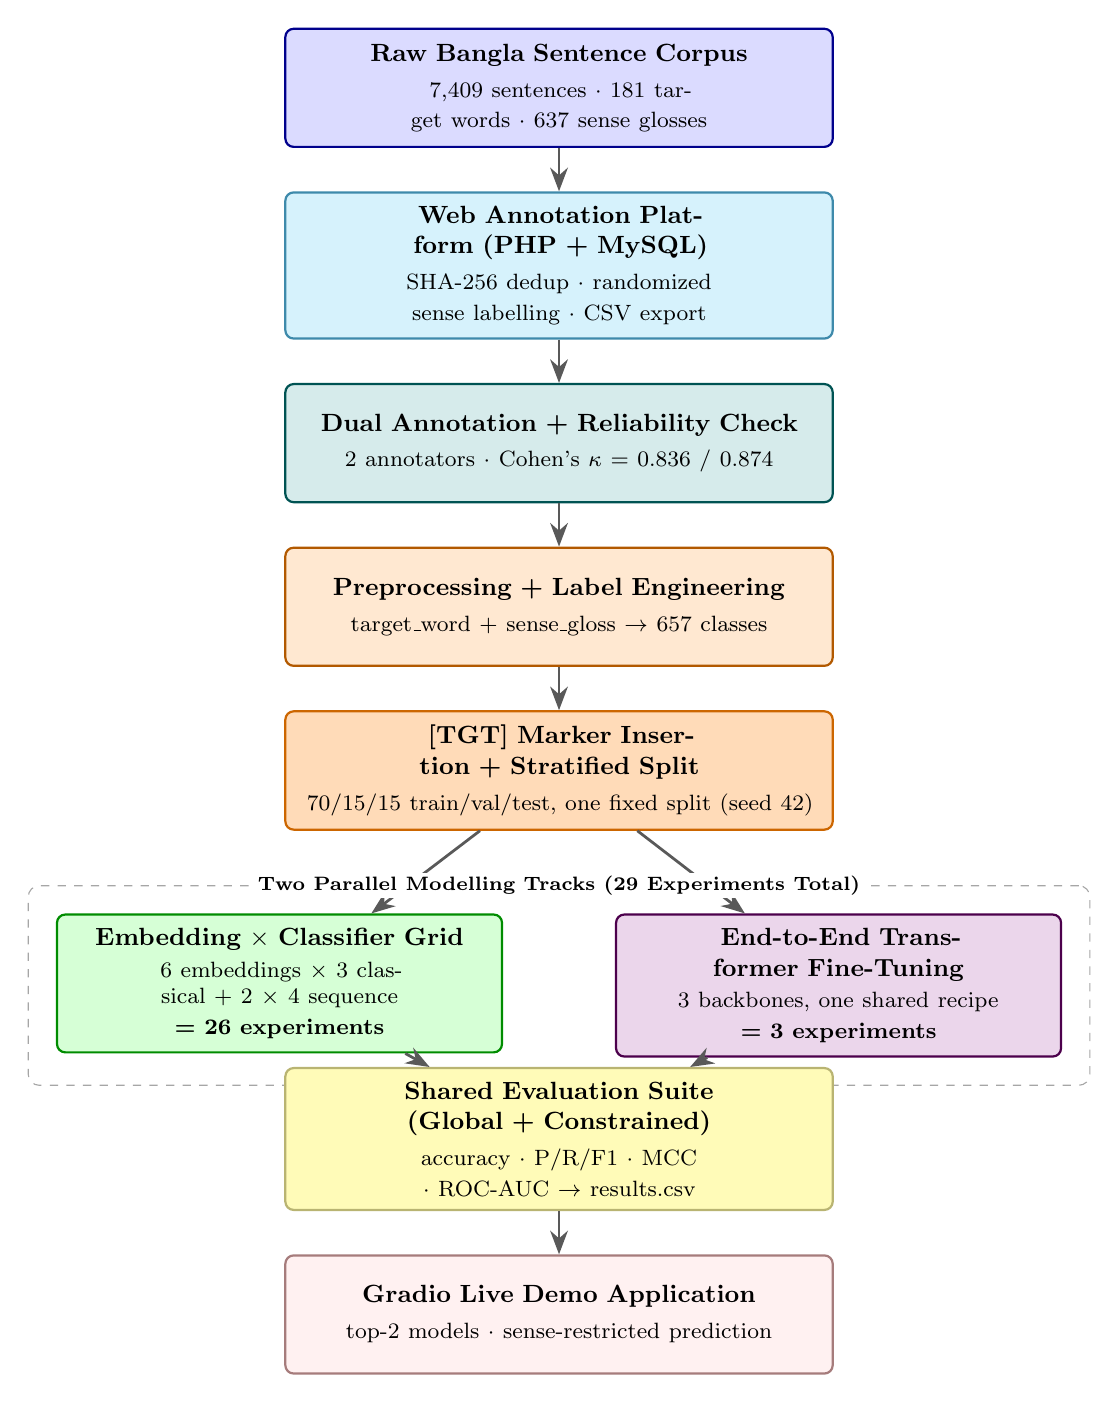
\begin{tikzpicture}[
  node distance=0.55cm,
  box/.style={draw=black!55, thick, rounded corners=3pt, align=center,
    minimum height=1.5cm, text width=6.6cm, inner sep=5pt,
    font=\fontsize{9}{11}\selectfont},
  narrowbox/.style={box, text width=5.3cm},
  arr/.style={-{Stealth[length=3mm]}, line width=1pt, draw=black!65},
  groupbox/.style={draw=black!35, dashed, rounded corners=4pt, inner sep=10pt}
]
\node[box, fill=blue!14, draw=blue!55!black] (raw)
  {\textbf{Raw Bangla Sentence Corpus}\\[2pt]
   \footnotesize 7{,}409 sentences $\cdot$ 181 target words $\cdot$ 637 sense glosses};
\node[box, fill=cyan!16, draw=cyan!65!black, below=of raw] (platform)
  {\textbf{Web Annotation Platform (PHP + MySQL)}\\[2pt]
   \footnotesize SHA-256 dedup $\cdot$ randomized sense labelling $\cdot$ CSV export};
\node[box, fill=teal!16, draw=teal!65!black, below=of platform] (kappa)
  {\textbf{Dual Annotation + Reliability Check}\\[2pt]
   \footnotesize 2 annotators $\cdot$ Cohen's $\kappa$ = 0.836 / 0.874};
\node[box, fill=orange!18, draw=orange!70!black, below=of kappa] (prep)
  {\textbf{Preprocessing + Label Engineering}\\[2pt]
   \footnotesize target\_word + sense\_gloss $\to$ 657 classes};
\node[box, fill=orange!28, draw=orange!80!black, below=of prep] (split)
  {\textbf{[TGT] Marker Insertion + Stratified Split}\\[2pt]
   \footnotesize 70/15/15 train/val/test, one fixed split (seed 42)};

\node[narrowbox, fill=green!16, draw=green!55!black, below=1.05cm of split, xshift=-3.55cm] (grid)
  {\textbf{Embedding $\times$ Classifier Grid}\\[2pt]
   \footnotesize 6 embeddings $\times$ 3 classical + 2 $\times$ 4 sequence\\ \textbf{= 26 experiments}};
\node[narrowbox, fill=violet!16, draw=violet!60!black, below=1.05cm of split, xshift=3.55cm] (ft)
  {\textbf{End-to-End Transformer Fine-Tuning}\\[2pt]
   \footnotesize 3 backbones, one shared recipe\\ \textbf{= 3 experiments}};

\begin{scope}[on background layer]
\node[groupbox, fit=(grid)(ft)] (trackbg) {};
\end{scope}

\node[box, fill=yellow!28, draw=yellow!55!black!70, below=3.0cm of split] (eval)
  {\textbf{Shared Evaluation Suite (Global + Constrained)}\\[2pt]
   \footnotesize accuracy $\cdot$ P/R/F1 $\cdot$ MCC $\cdot$ ROC-AUC $\to$ results.csv};
\node[box, fill=pink!22, draw=pink!65!black, below=of eval] (demo)
  {\textbf{Gradio Live Demo Application}\\[2pt]
   \footnotesize top-2 models $\cdot$ sense-restricted prediction};

\draw[arr] (raw) -- (platform);
\draw[arr] (platform) -- (kappa);
\draw[arr] (kappa) -- (prep);
\draw[arr] (prep) -- (split);
\draw[arr] (split) -- (grid);
\draw[arr] (split) -- (ft);
\node[font=\bfseries\fontsize{7.5}{9}\selectfont, fill=white, inner sep=1pt] at (trackbg.north) {Two Parallel Modelling Tracks (29 Experiments Total)};
\draw[arr] (grid) -- (eval);
\draw[arr] (ft) -- (eval);
\draw[arr] (eval) -- (demo);
\end{tikzpicture}}
\caption{Overall system architecture of the proposed Bangla WSD framework.}
\label{fig:pipeline_overview}
\end{figure}
\section{Bangla WSD Dataset}
{\fontsize{12}{18}\selectfont\normalfont\setstretch{1.5}\justifying\sloppy\emergencystretch=3em
The corpus underlying this thesis originates from dataset\_updated.xlsx (7,409 rows), compiled specifically for this work rather than adapted from an existing Bangla NLP resource. Each row of the file is one annotated example, described by five fields: word\_id, a numeric identifier of the polysemous target word; target\_word, the surface form of that word; sense\_id, the index of the sense assigned to this particular occurrence (unique only within its target word, a property whose consequences Section 3.5 addresses); sense\_gloss, a short Bangla gloss defining that sense; and text, the complete example sentence in which the target word is used in that sense. Table 3.1 reproduces a sample of annotated rows for one representative target word, \bn{জল}, showing two example sentences for each of its three senses so that the (target\_word, sense\_gloss, text) structure of a row is concrete before the aggregate statistics below. Figure 3.2 then gives a composition overview of the raw corpus along four complementary axes, Figure 3.3 summarises the five-step process by which the corpus was built, from the selection of genuinely polysemous target words through to the final validated collection of sense-labelled sentences, and Table 3.2 reports the resulting corpus-level totals. A larger sample of the corpus file itself, one example sentence per sense for six representative target words, is reproduced verbatim in Appendix A (Table A.1). Section 3.3 then describes the web annotation platform through which the human labelling step (the final stage of Figure 3.3) was actually carried out.\par

}
\begin{table}[htbp]
\caption{Sample annotated rows for the target word \bn{জল} (word\_id 1), two example sentences per sense.}
\label{tab:dataset_sample}
\centering
{\fontsize{10}{14}\selectfont
\begin{tabular}{@{}p{1.4cm} p{3.1cm} p{9.9cm}@{}}
\toprule
\textbf{Sense ID} & \textbf{Sense Gloss} & \textbf{Example Sentence (text)} \\
\midrule
\multirow{2}{*}{1} & \multirow{2}{*}{\bn{অত্যাধিক পরিশ্রম}} & \bn{মাঠে সারাদিন রক্ত জল করা পরিশ্রম করেও কৃষক ন্যায্য মূল্য থেকে বঞ্চিত হন।} \\
\addlinespace[3pt]
 & & \bn{বছরের পর বছর রক্ত জল করা পরিশ্রম করে তিনি এই কারখানাটি দাঁড় করিয়েছেন।} \\
\addlinespace[6pt]
\multirow{2}{*}{2} & \multirow{2}{*}{\bn{বৃষ্টি}} & \bn{আকাশভরা কালো মেঘ দেখে মনে হচ্ছে আজ প্রচণ্ড জল পড়বে।} \\
\addlinespace[3pt]
 & & \bn{কৃষকরা জল পড়ার অপেক্ষায় আকাশের দিকে তাকিয়ে আছেন কারণ ফসলের মাঠ শুকিয়ে গেছে।} \\
\addlinespace[6pt]
\multirow{2}{*}{3} & \multirow{2}{*}{\bn{অশ্রু}} & \bn{সন্তানের বিদেশযাত্রার দিন মা চোখের জল আর আটকে রাখতে পারলেন না।} \\
\addlinespace[3pt]
 & & \bn{প্রিয় বন্ধুর মৃত্যুসংবাদ শুনে তার চোখ থেকে অনবরত জল পড়তে লাগল।} \\
\addlinespace[3pt]
\bottomrule
\end{tabular}}
\end{table}
\begin{figure}[htbp]
\centering
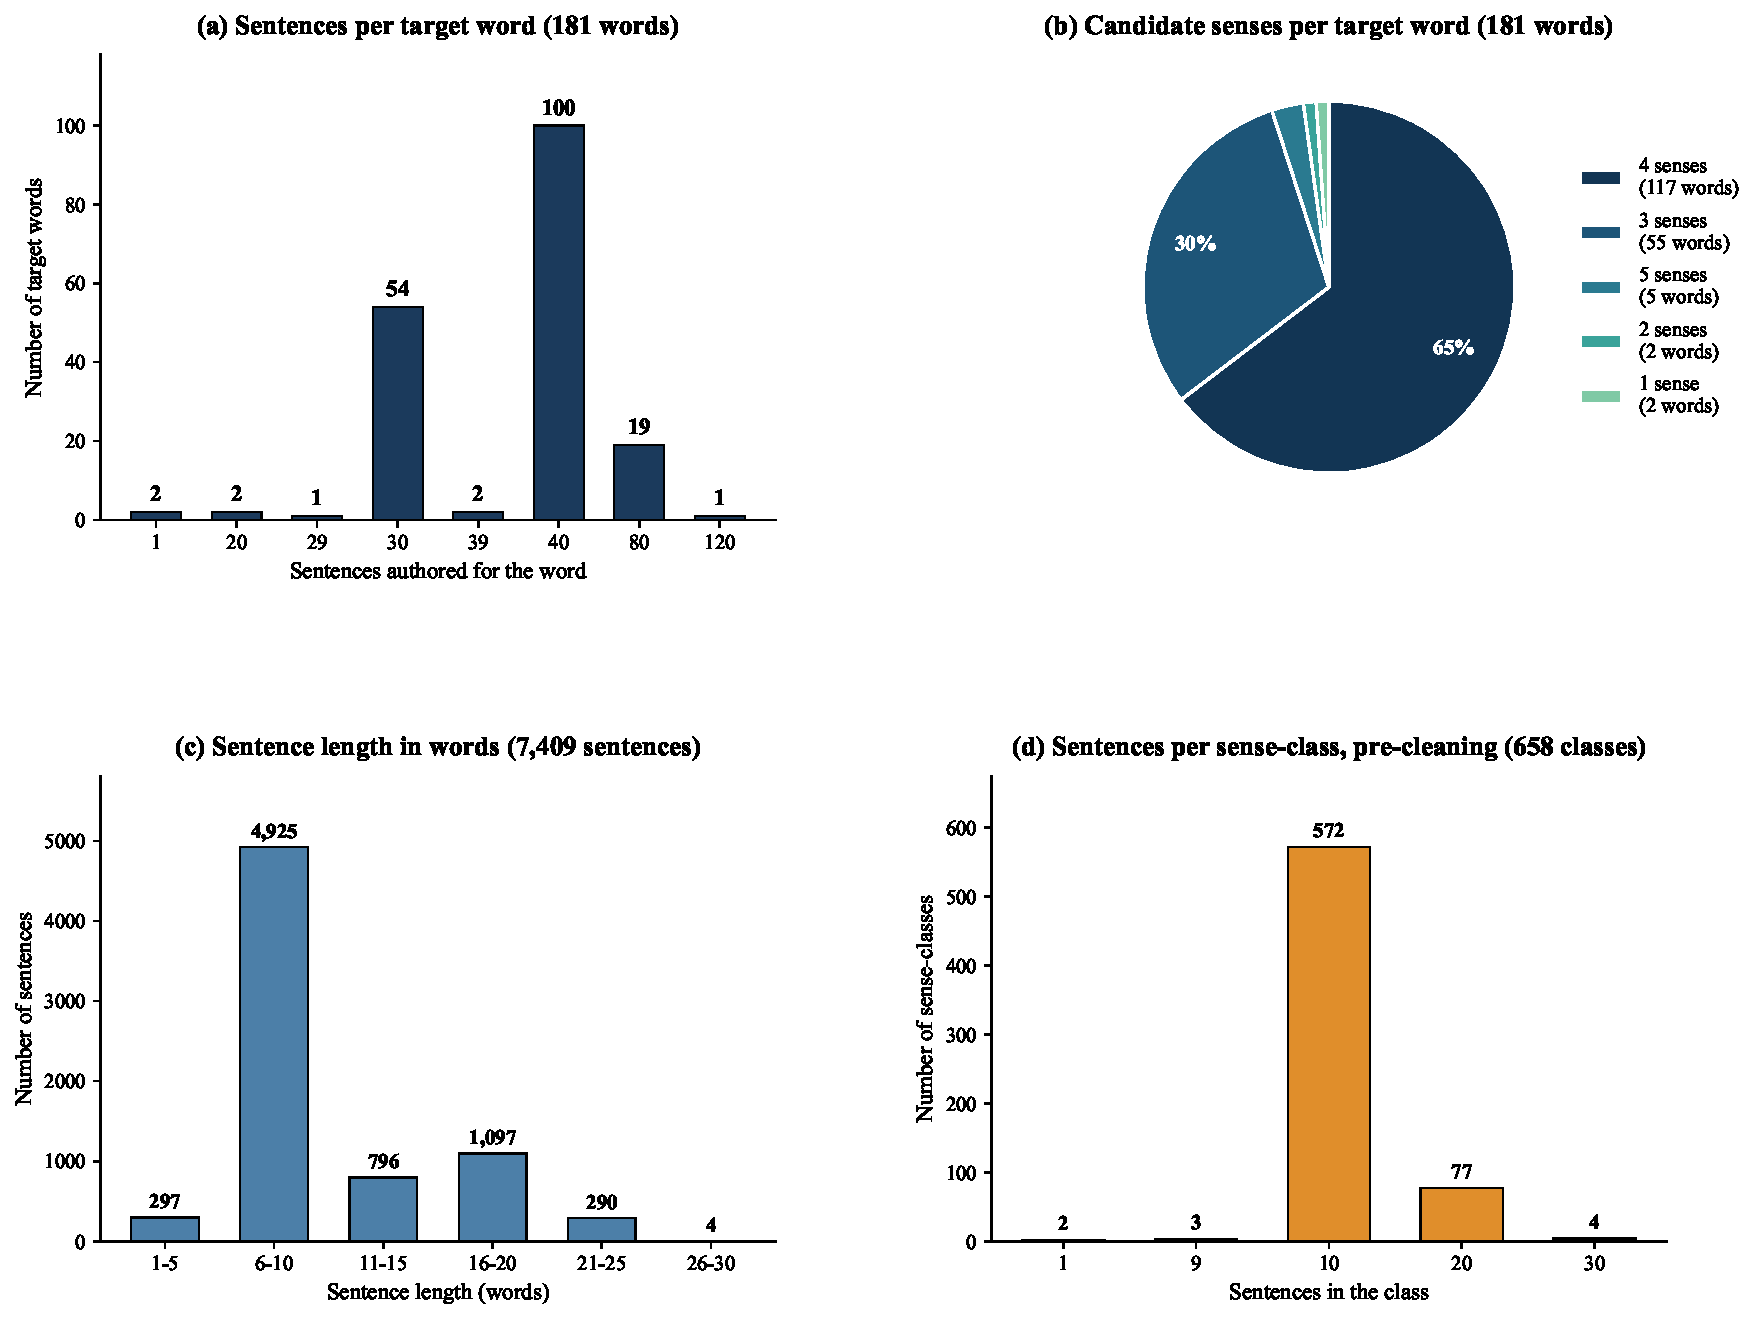
\includegraphics[width=0.92\textwidth]{details/figures/dataset_composition_overview.pdf}
\caption{Bangla WSD corpus composition overview: (a) sentences per target word, (b) senses per target word, (c) sentence length, (d) sentences per sense-class.}
\label{fig:dataset_composition_overview}
\end{figure}
{\fontsize{12}{18}\selectfont\normalfont\setstretch{1.5}\justifying\sloppy\emergencystretch=3em
Figure 3.2b shows that the raw corpus is not evenly distributed across sense counts: of the 181 target words, 117 are defined with exactly four candidate senses, 55 with three, five with five, and two each with one or two senses, so the typical annotation decision facing an annotator is a three- or four-way choice rather than a binary one, which is itself a source of potential disagreement that motivates the reliability check described in Section 3.3. Sentence allocation across the 181 words is likewise not uniform (Figure 3.2a): 100 words received the default 40 example sentences and 54 received 30, but 19 higher-frequency words were extended to 80 sentences and one, \bn{ধারা}, to 120, while two placeholder words carry only a single sentence each -- consistent with the 181-to-179 drop in target-word count that the Section 3.4 preprocessing pipeline's rare-sense filter later produces (Section 3.5). Sentence length is concentrated in the 6-10 word range (4,925 of 7,409 sentences, Figure 3.2c), consistent with the short, single-clause example sentences the annotation guidelines asked contributors to write. Finally, Figure 3.2d shows that the 658 raw (word, sense) classes are already close to balanced before Section 3.4's cleaning pass, with 572 classes holding exactly 10 sentences and a further 77 holding 20; only 9 classes (2 with a single sentence, 3 with 9, and 4 with 30) fall outside this pattern, which is why the downstream classifiers in Chapter 4 require no explicit class-imbalance handling.\par

}
\subsection{Dataset Description}
{\fontsize{12}{18}\selectfont\normalfont\setstretch{1.5}\justifying\sloppy\emergencystretch=3em
The dataset used throughout this thesis is a custom-built Bangla WSD resource constructed specifically for this research rather than an adaptation of any existing corpus. Its construction followed the five-step process illustrated in Figure 3.3: a set of genuinely polysemous Bangla target words was first selected; the candidate senses of each word were then defined as short Bangla glosses; realistic example sentences were collected for every sense of every word; the material was structured into the five-field spreadsheet format described at the start of this section; and, finally, every sentence was manually labelled with the sense it expresses by two independent human annotators through the web annotation platform of Section 3.3. The resulting labelled corpus is later divided into training, validation, and test sets (Section 3.7) for model training and evaluation. Table 3.2 summarises the principal characteristics of the dataset.\par

}
\vspace{10pt}
\begin{figure}[htbp]
\centering
\resizebox{0.92\textwidth}{!}{%
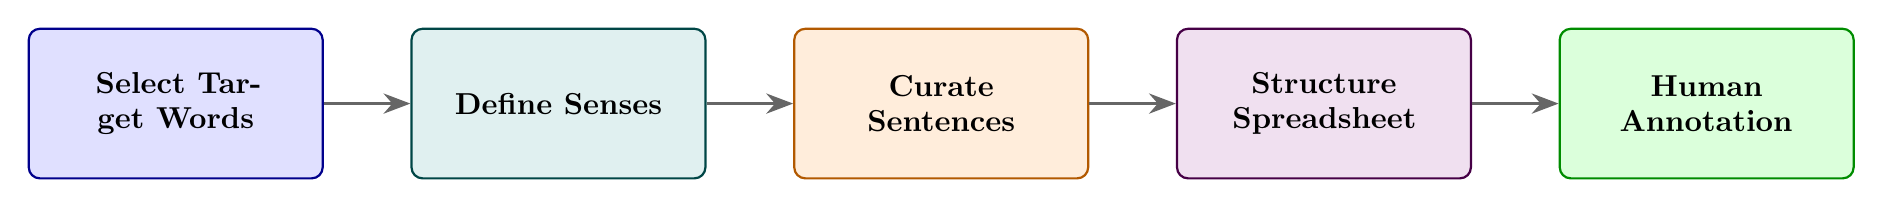
\begin{tikzpicture}[
  node distance=1.1cm,
  stepbox/.style={draw=black!55, thick, rounded corners=4pt, align=center, fill=white,
    minimum height=1.9cm, text width=3.1cm, inner sep=9pt, font=\bfseries\fontsize{10.5}{12.5}\selectfont},
  arr/.style={-{Stealth[length=3.4mm]}, line width=1.3pt, draw=black!60}
]
\node[stepbox, fill=blue!12, draw=blue!55!black] (s1)
  {Select Target Words};
\node[stepbox, fill=teal!12, draw=teal!55!black, right=of s1] (s2)
  {Define Senses};
\node[stepbox, fill=orange!14, draw=orange!70!black, right=of s2] (s3)
  {Curate Sentences};
\node[stepbox, fill=violet!12, draw=violet!55!black, right=of s3] (s4)
  {Structure Spreadsheet};
\node[stepbox, fill=green!14, draw=green!55!black, right=of s4] (s5)
  {Human Annotation};

\draw[arr] (s1) -- (s2);
\draw[arr] (s2) -- (s3);
\draw[arr] (s3) -- (s4);
\draw[arr] (s4) -- (s5);
\end{tikzpicture}}
\caption{Five-step Bangla dataset creation process.}
\label{fig:dataset_overview}
\end{figure}
\vspace{10pt}
\begin{table}[htbp]
\caption{Description of the annotated Bangla WSD corpus.}
\label{tab:dataset_stats}
\centering
{\fontsize{10}{14}\selectfont
\begin{tabular}{@{}p{7.60cm} p{6.10cm}@{}}
\toprule
\textbf{Characteristic} & \textbf{Description} \\
\midrule
Dataset type & Sense-annotated Bangla WSD corpus (lexical-sample) \\
\addlinespace[3pt]
Language & Bangla (Bengali) \\
\addlinespace[3pt]
Annotation & Manual, by two independent annotators \\
\addlinespace[3pt]
File format & Excel spreadsheet (dataset\_updated.xlsx) \\
\addlinespace[3pt]
Target (polysemous) words & 181 \\
\addlinespace[3pt]
Raw annotated sentences & 7,409 \\
\addlinespace[3pt]
Candidate sense glosses & 637 \\
\addlinespace[3pt]
Average senses per target word & 3.67 \\
\addlinespace[3pt]
Average sentences per sense class & 11.3 \\
\addlinespace[3pt]
Final classes (post-cleaning) & 657 \\
\addlinespace[3pt]
\bottomrule
\end{tabular}}
\end{table}
\section{Web Annotation Platform}
{\fontsize{12}{18}\selectfont\normalfont\setstretch{1.5}\justifying\sloppy\emergencystretch=3em
The 7,409 sentences described in Section 3.2 are labelled through a purpose-built PHP/MySQL web annotation platform written for this thesis rather than an offline script. An administrator imports the spreadsheet (import\_dataset.php), which computes a SHA-256 hash per row to prevent duplicate import. Annotators register and log in (bcrypt-hashed passwords, session regeneration on login) and label one sentence at a time (annotation.php): the target word is highlighted in the sentence and its candidate senses are presented in randomized order to reduce positional bias. Submissions are stored per annotator under a unique (sentence\_id, annotator\_id) database constraint, so each annotator labels a given sentence exactly once; skipped sentences are deferred to the end of the session queue. The administrator dashboard tracks per-annotator progress and exports an aligned CSV (export\_csv.php) once annotation is complete. Figure 3.4 details the internal workflow of the platform, corresponding to the final stage of the dataset creation process in Figure 3.3.\par

}
\begin{figure}[htbp]
\centering
\resizebox{\textwidth}{!}{%
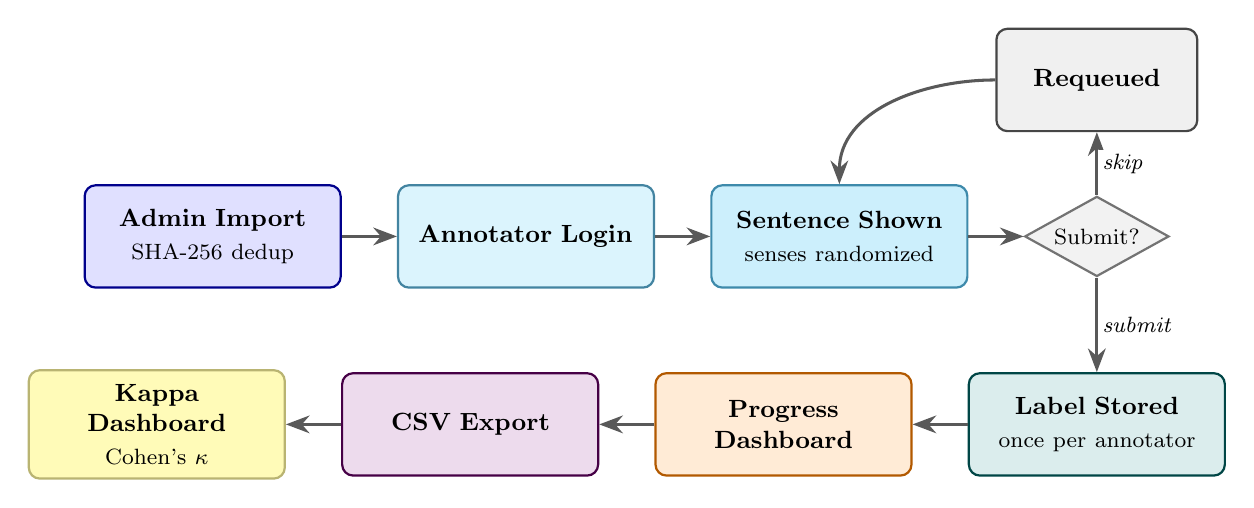
\begin{tikzpicture}[
  node distance=1.0cm and 0.7cm,
  box/.style={draw=black!55, thick, rounded corners=4pt, align=center, fill=white,
    minimum height=1.3cm, text width=2.9cm, inner sep=5pt, font=\fontsize{9}{11}\selectfont},
  decision/.style={draw=black!55, thick, diamond, aspect=1.8, align=center, inner sep=2pt,
    font=\fontsize{8.5}{10}\selectfont, fill=gray!10},
  arr/.style={-{Stealth[length=3mm]}, line width=1.1pt, draw=black!65},
  lbl/.style={font=\fontsize{8}{9}\selectfont\itshape, fill=white, inner sep=1.5pt}
]
% Top row: import to labelling
\node[box, fill=blue!12, draw=blue!55!black] (import) {\textbf{Admin Import}\\[1pt]\footnotesize SHA-256 dedup};
\node[box, fill=cyan!14, draw=cyan!60!black, right=of import] (login) {\textbf{Annotator Login}};
\node[box, fill=cyan!20, draw=cyan!65!black, right=of login] (present) {\textbf{Sentence Shown}\\[1pt]\footnotesize senses randomized};
\node[decision, right=of present] (dec) {Submit?};
\node[box, fill=gray!12, draw=gray!55!black, above=0.8cm of dec, text width=2.2cm] (skip) {\textbf{Requeued}};

% Bottom row: storage to reliability dashboard (right to left)
\node[box, fill=teal!14, draw=teal!55!black, below=1.2cm of dec] (store) {\textbf{Label Stored}\\[1pt]\footnotesize once per annotator};
\node[box, fill=orange!16, draw=orange!70!black, left=of store] (progress) {\textbf{Progress Dashboard}};
\node[box, fill=violet!14, draw=violet!55!black, left=of progress] (export) {\textbf{CSV Export}};
\node[box, fill=yellow!28, draw=yellow!55!black!70, left=of export] (kappadash) {\textbf{Kappa Dashboard}\\[1pt]\footnotesize Cohen's $\kappa$};

\draw[arr] (import) -- (login);
\draw[arr] (login) -- (present);
\draw[arr] (present) -- (dec);
\draw[arr] (dec) -- node[lbl, right] {skip} (skip);
\draw[arr] (skip.west) to[out=180, in=90] (present.north);
\draw[arr] (dec) -- node[lbl, right] {submit} (store);
\draw[arr] (store) -- (progress);
\draw[arr] (progress) -- (export);
\draw[arr] (export) -- (kappadash);
\end{tikzpicture}}
\caption{Workflow of the web annotation platform.}
\label{fig:annotation_flowchart}
\end{figure}
{\fontsize{12}{18}\selectfont\normalfont\setstretch{1.5}\justifying\sloppy\emergencystretch=3em
\subsection{Reliability Statistic: Cohen's Kappa}

Because every downstream experiment in Chapters 3-4 is trained on labels that two human annotators assigned independently, the reliability of those labels must be quantified before they are trusted as ground truth. This thesis follows Cohen \cite{cohen1960kappa} and computes, for each annotator, agreement against the gold sense recorded on the platform:

\begin{equation}
\kappa = \frac{p_o - p_e}{1 - p_e}
\label{eq:kappa}
\end{equation}

where \(p_o\) is the observed proportion of sentences on which the annotator's chosen sense matches the gold sense, and \(p_e\) is the proportion of agreement expected by chance alone. \(p_e\) is computed from the marginal sense-frequency distribution of the confusion matrix between annotator and gold labels,

\begin{equation}
p_e = \sum_{k=1}^{K} p_k^{(a)} \, p_k^{(g)}
\label{eq:kappa_pe}
\end{equation}

where \(K\) is the number of candidate senses for the target word under consideration, \(p_k^{(a)}\) is the proportion of the annotator's labels falling in sense \(k\), and \(p_k^{(g)}\) is the corresponding proportion in the gold labels; \(\kappa\) therefore corrects raw percentage agreement (\(p_o\)) for the agreement that would occur even if the annotator were labelling at random with the same marginal sense frequencies. Because \(\kappa \le p_o\) whenever \(p_e > 0\), it is a strictly more conservative and informative statistic than accuracy alone, which is why it is adopted here rather than a simple agreement percentage. The evaluation.php dashboard invokes kappa.py against the exported annotation CSV to compute Equations \ref{eq:kappa}-\ref{eq:kappa_pe} per annotator; the resulting values are reported in Section 4.3 and interpreted using the Landis and Koch \cite{landis1977kappa} ordinal agreement scale reproduced in Table 3.3.\par

}
\begin{table}[htbp]
\caption{Landis and Koch (1977) interpretation scale for Cohen's Kappa.}
\label{tab:kappa_scale}
\centering
{\fontsize{10}{14}\selectfont
\begin{tabular}{@{}p{3.90cm} p{8.10cm}@{}}
\toprule
\textbf{\(\kappa\) range} & \textbf{Strength of agreement} \\
\midrule
\(< 0.00\) & Poor (worse than chance) \\
\addlinespace[3pt]
\(0.00\text{--}0.20\) & Slight \\
\addlinespace[3pt]
\(0.21\text{--}0.40\) & Fair \\
\addlinespace[3pt]
\(0.41\text{--}0.60\) & Moderate \\
\addlinespace[3pt]
\(0.61\text{--}0.80\) & Substantial \\
\addlinespace[3pt]
\(0.81\text{--}1.00\) & Almost perfect \\
\addlinespace[3pt]
\bottomrule
\end{tabular}}
\end{table}
{\fontsize{12}{18}\selectfont\normalfont\setstretch{1.5}\justifying\sloppy\emergencystretch=3em
}
\section{Preprocessing Pipeline}
{\fontsize{12}{18}\selectfont\normalfont\setstretch{1.5}\justifying\sloppy\emergencystretch=3em
Preprocessing, applied identically across all downstream experiments, removes rows with missing fields, normalises whitespace, discards sentences shorter than five characters, verifies that the target word literally occurs in its sentence (a sample cannot be marked otherwise; see Section 3.6), removes duplicate (text, sense\_id, target\_word) rows, and finally discards senses supported by fewer than three examples (MIN\_SAMPLES = 3), since a class cannot be stratified into train/validation/test with fewer samples. Table 3.4 reports the exact row counts removed at each step, as printed by the pipeline, and Figure 3.5 plots the same counts to make the (small) magnitude of each drop visually obvious against the 7,409-row starting point.\par

}
\begin{table}[htbp]
\caption{Preprocessing pipeline, rows removed at each step.}
\label{tab:auto11}
\centering
{\fontsize{10}{14}\selectfont
\begin{tabular}{@{}p{2.60cm} p{5.84cm} p{5.84cm}@{}}
\toprule
\textbf{Step} & \textbf{Rows Dropped} & \textbf{Rows Remaining} \\
\midrule
Initial load & - & 7,409 \\
\addlinespace[3pt]
NaN / empty-text removal & 0 & 7,409 \\
\addlinespace[3pt]
Target-word-in-text validation & 19 & 7,390 \\
\addlinespace[3pt]
Duplicate removal & 1 & 7,389 \\
\addlinespace[3pt]
Rare-sense filter (< 3 samples) & 8 & 7,381 \\
\addlinespace[3pt]
\bottomrule
\end{tabular}}
\end{table}
{\fontsize{12}{18}\selectfont\normalfont\setstretch{1.5}\justifying\sloppy\emergencystretch=3em
Every step other than the rare-sense filter removes fewer than 20 rows out of 7,409, evidence that dataset\_updated.xlsx was already largely clean at export time and that the annotation platform's SHA-256 de-duplication (Section 3.3, Figure 3.4) had already prevented most redundant submissions before they reached the spreadsheet.\par

}
\begin{figure}[htbp]
\centering
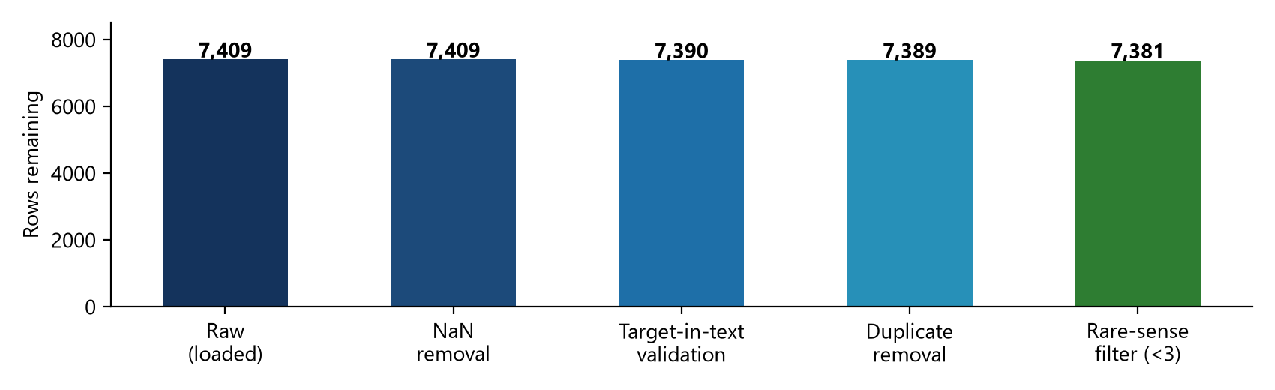
\includegraphics[width=0.85\textwidth]{details/figures/preprocessing_rows_chart.pdf}
\caption{Rows remaining after each preprocessing step.}
\label{fig:preprocessing_rows}
\end{figure}
\section{Word-Specific Label Construction}
{\fontsize{12}{18}\selectfont\normalfont\setstretch{1.5}\justifying\sloppy\emergencystretch=3em
The raw sense\_id (values 1-4) collides across target words: sense\_id = 1 means "colour" for \bn{বর্ণ} but "body part" for \bn{হাত}. Following the design decision central to this thesis, each label is instead built as target\_word + "\_" + sense\_gloss, producing a unique, non-colliding string per (word, sense) pair, encoded to an integer via scikit-learn's LabelEncoder. After the rare-sense filter, this yields 657 unique classes across 179 target words, all trained as one global 657-way classification problem rather than 179 separate per-word classifiers. A word-to-label-indices mapping is retained purely for inference-time sense-restriction (Section 3.11) and does not alter the training objective.\par

}
\section{[TGT] Marker Insertion}
{\fontsize{12}{18}\selectfont\normalfont\setstretch{1.5}\justifying\sloppy\emergencystretch=3em
Transformers attend to all input tokens with no built-in notion of which word is being disambiguated. To direct attention, the first occurrence of the target word in each sentence is wrapped in the markers [TGT] and [/TGT] (e.g. \bn{তার চোখে জল এলো} becomes \bn{তার চোখে} [TGT] \bn{জল} [/TGT] \bn{এলো}). Crucially, both markers are registered as genuine tokenizer special tokens (via add\_special\_tokens(), followed by resize\_token\_embeddings() on the model) for every transformer backbone, frozen and fine-tuned alike, so that each marker maps to exactly one atomic, stable token id. Left as plain literal text, the markers would instead be fragmented into several inconsistent sub-word pieces; XLM-R's SentencePiece tokenizer, for example, splits the literal string ``[TGT]'' into four context-dependent pieces, destroying the marker's value as a stable attention signal (a failure mode analysed further in Section 4.5). The same insert\_tgt\_markers() function and the same special-token registration are reused unchanged between the training pipeline and the live demo application (Section 3.11), so training-time and inference-time preprocessing cannot diverge.\par

}
\section{Stratified Data Splitting}
{\fontsize{12}{18}\selectfont\normalfont\setstretch{1.5}\justifying\sloppy\emergencystretch=3em
Each of the 657 classes is split 70/15/15 into train/validation/test using scikit-learn's stratified train\_test\_split with seed 42, so every class appears in all three subsets at roughly its full-dataset proportion; because every post-filter class holds at least seven examples, the full three-way stratification succeeds with all 657 classes present in each subset. Exactly one fixed split is used, and every one of the twenty-nine experiments, classical, sequence, and fine-tuned alike, trains and is evaluated on this identical partition, so that no accuracy difference between any two configurations can be an artefact of the data they received. The split indices are persisted to disk (split\_info.json) for reproducibility and auditing. Table 3.5 reports the resulting sizes.\par

}
\begin{table}[htbp]
\caption{Stratified split sizes (out of 7,381 rows, 657 classes).}
\label{tab:auto12}
\centering
{\fontsize{10}{14}\selectfont
\begin{tabular}{@{}p{2.60cm} p{3.75cm} p{3.75cm} p{3.75cm}@{}}
\toprule
\textbf{Split} & \textbf{Rows} & \textbf{Percentage} & \textbf{Classes Present} \\
\midrule
Train & 5,166 & 70.0\% & 657 / 657 \\
\addlinespace[3pt]
Validation & 1,107 & 15.0\% & 657 / 657 \\
\addlinespace[3pt]
Test & 1,108 & 15.0\% & 657 / 657 \\
\addlinespace[3pt]
\bottomrule
\end{tabular}}
\end{table}
{\fontsize{12}{18}\selectfont\normalfont\setstretch{1.5}\justifying\sloppy\emergencystretch=3em
}
\section{Embedding Generation and Classifier Grid}
{\fontsize{12}{18}\selectfont\normalfont\setstretch{1.5}\justifying\sloppy\emergencystretch=3em
Six embedding families are generated and disk-cached, each following the same fit-on-train, transform-all contract. TF-IDF (word 1--2-grams, 30,000 max features, sublinear term frequency, sparse) is fitted on the training split only. Word2Vec and fastText are deliberately \emph{not} trained on the WSD corpus itself: 7,381 sentences are far too few to learn meaningful distributional vectors, so the pretrained 100-dimensional Bangla Word2Vec model of sagorsarker/bangla\_word2vec \cite{mikolov2013word2vec} and the official pretrained 300-dimensional Bengali fastText vectors \cite{bojanowski2017fasttext} (whose sub-word n-grams generate genuine vectors even for out-of-vocabulary inflected forms) are loaded instead, with measured train-token coverage above 98\% and 97\% respectively. For the classical learners, both static embeddings are turned into a target-aware representation, the concatenation [left-context; target word; right-context] with a five-word context window on each side, rather than a whole-sentence mean that would dilute the disambiguation signal. The three transformer backbones, bert-base-multilingual-cased (mBERT), sagorsarker/bangla-bert-base (BanglaBERT), and xlm-roberta-base (XLM-R), contribute frozen embeddings formed as the concatenation of the [CLS] vector and the mean of the hidden states over the [TGT]-marked target span (1,536 dimensions), with no fine-tuning at this stage. Three classical learners (Naive Bayes, Logistic Regression, Linear SVM) are trained on all six embeddings via a single reusable train\_and\_evaluate\_classical() function, giving eighteen experiments. The four recurrent architectures (LSTM, GRU, BiLSTM, BiGRU), instantiated from one generic SequenceClassifier module (hidden size 128, batch size 32, learning rate 1e-3, up to 30 epochs with early-stopping patience 5), are trained only on Word2Vec and fastText, the two embeddings with genuine per-token sequence structure (padded/truncated to 21 tokens, the 95th percentile of training-sentence length); feeding a recurrent model a single pooled TF-IDF or [CLS] vector at sequence length one is not genuine sequence modelling, so those combinations are excluded rather than kept as invalid comparison points. This gives eight sequence experiments, and 18 + 8 = 26 grid experiments in total, all on the single fixed split of Section 3.7.\par

}
\section{Transformer Fine-Tuning}
{\fontsize{12}{18}\selectfont\normalfont\setstretch{1.5}\justifying\sloppy\emergencystretch=3em
The remaining three experiments fine-tune mBERT, BanglaBERT, and XLM-R end-to-end. Each backbone (loaded via HuggingFace AutoModel) feeds its 768-dimensional [CLS] representation through an identical classification head: LayerNorm, Dropout(0.3), Linear(768,768), GELU, Dropout(0.3), Linear(768,657), softmax. Figure 3.6 diagrams this shared head, from the fine-tuned backbone through to the final 657-way sense prediction; the embedding-only experiments of Section 3.8 instead keep the backbone frozen, extract the 1,536-D [CLS]+target-span vector, and feed it to the classical learners of that section. Table 3.6 lists the shared training configuration, identical across all three backbones so that any accuracy difference reflects the backbone rather than the recipe. Before each run, a diagnostic block verifies the label mapping (min/max label id versus classifier output size), the tokenizer/model vocabulary consistency after the special-token registration of Section 3.6, and the gradient flow into the backbone, so that a training failure cannot silently stem from a plumbing defect.\par

}
\begin{figure}[htbp]
\centering
\resizebox{\textwidth}{!}{%
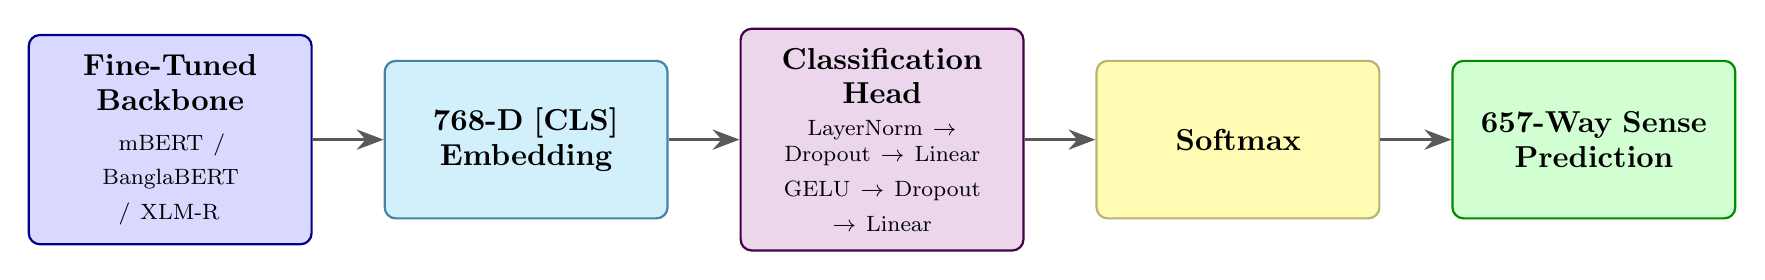
\begin{tikzpicture}[
  node distance=0.9cm,
  headbox/.style={draw=black!55, thick, rounded corners=4pt, align=center, fill=white,
    minimum height=2.0cm, text width=3.1cm, inner sep=7pt, font=\fontsize{10.5}{12.5}\selectfont},
  arr/.style={-{Stealth[length=3.4mm]}, line width=1.3pt, draw=black!65}
]
\node[headbox, fill=blue!15, draw=blue!55!black] (backbone)
  {\bfseries Fine-Tuned Backbone\\[2pt]\normalfont\footnotesize mBERT / BanglaBERT / XLM-R};
\node[headbox, fill=cyan!18, draw=cyan!60!black, right=of backbone] (cls)
  {\bfseries 768-D {[}CLS{]} Embedding};
\node[headbox, fill=violet!16, draw=violet!55!black, right=of cls] (head)
  {\bfseries Classification Head\\[2pt]\normalfont\footnotesize LayerNorm $\rightarrow$ Dropout $\rightarrow$ Linear\\ GELU $\rightarrow$ Dropout $\rightarrow$ Linear};
\node[headbox, fill=yellow!30, draw=yellow!55!black!70, right=of head] (softmax)
  {\bfseries Softmax};
\node[headbox, fill=green!18, draw=green!55!black, right=of softmax] (output)
  {\bfseries 657-Way Sense Prediction};

\draw[arr] (backbone) -- (cls);
\draw[arr] (cls) -- (head);
\draw[arr] (head) -- (softmax);
\draw[arr] (softmax) -- (output);
\end{tikzpicture}}
\caption{Shared transformer classification head, applied identically on top of all three fine-tuned backbones.}
\label{fig:finetune_head}
\end{figure}
\begin{table}[htbp]
\caption{Shared fine-tuning configuration, identical for all three backbones.}
\label{tab:auto13}
\centering
{\fontsize{10}{14}\selectfont
\begin{tabular}{@{}p{4.20cm} p{10.50cm}@{}}
\toprule
\textbf{Hyperparameter} & \textbf{Value} \\
\midrule
Max sequence length & 128 tokens \\
\addlinespace[3pt]
Batch size & 16 \\
\addlinespace[3pt]
Optimizer & AdamW, weight decay 0.01 \\
\addlinespace[3pt]
Learning rate (backbone / head) & 2e-5 / 2e-4 (10x discriminative) \\
\addlinespace[3pt]
LR schedule & Linear warm-up, 10\% of steps \\
\addlinespace[3pt]
Loss & Weighted cross-entropy (class-balanced) \\
\addlinespace[3pt]
Gradient clipping & max\_norm = 1.0 \\
\addlinespace[3pt]
Mixed precision & Enabled (torch.cuda.amp) \\
\addlinespace[3pt]
Max epochs / patience & 15 / 4 (early stopping) \\
\addlinespace[3pt]
Random seed & 42 (same fixed split as all other experiments) \\
\addlinespace[3pt]
\bottomrule
\end{tabular}}
\end{table}
{\fontsize{12}{18}\selectfont\normalfont\setstretch{1.5}\justifying\sloppy\emergencystretch=3em
Class-balanced loss weights (sklearn's compute\_class\_weight('balanced')) mitigate the 657-class imbalance, since the smallest classes contribute only about five training sentences each (seven examples in total before the 70/15/15 split). The optimizer is discriminative: the randomly initialised classification head receives ten times the backbone learning rate (2e-4 versus 2e-5), so the head can adapt quickly while the pretrained encoder moves conservatively. Training runs on a Tesla T4 GPU (15.6 GB VRAM) using PyTorch with mixed precision; the checkpoint with the best validation accuracy is restored before the final test-set evaluation reported in Section 4.5, and the test split is never used for model selection.\par

}
\section{Evaluation Metric Suite}
{\fontsize{12}{18}\selectfont\normalfont\setstretch{1.5}\justifying\sloppy\emergencystretch=3em
Every one of the twenty-nine experiments is scored on an identical, shared metric suite computed only on the held-out test split: accuracy; macro- and weighted-averaged precision, recall, and F1; balanced accuracy; Matthews correlation coefficient; Cohen's Kappa (as a model agreement statistic, distinct from the annotation-reliability Kappa of Section 3.3); macro- and weighted-averaged ROC-AUC; and a set of computational-cost metrics, training/validation/inference time, inference time per sample, trainable and total parameter counts, model size on disk, and peak GPU/CPU memory. All columns are written to a shared results CSV used throughout Chapter 4 and by the live demo application. The formulas below define each classification metric precisely, since the 657-class, imbalanced setting of this thesis makes the distinction between macro- and weighted-averaging, and between accuracy and balanced accuracy, materially important rather than a matter of reporting style.\par

For a test set of \(N\) sentences and \(K = 657\) classes, let \(\mathrm{TP}_k\), \(\mathrm{FP}_k\), and \(\mathrm{FN}_k\) denote the true positives, false positives, and false negatives for class \(k\), and let \(n_k\) be the number of test sentences whose gold label is \(k\) (so \(\sum_k n_k = N\)). Overall accuracy is the fraction of sentences assigned their exact gold sense:

\begin{equation}
\mathrm{Accuracy} = \frac{1}{N}\sum_{i=1}^{N} \mathbb{1}\!\left[\hat{y}_i = y_i\right].
\label{eq:accuracy}
\end{equation}

Per-class precision and recall,

\begin{equation}
P_k = \frac{\mathrm{TP}_k}{\mathrm{TP}_k + \mathrm{FP}_k}, \qquad
R_k = \frac{\mathrm{TP}_k}{\mathrm{TP}_k + \mathrm{FN}_k},
\label{eq:precision_recall}
\end{equation}

combine into the per-class F1 score \(F1_k = 2 P_k R_k / (P_k + R_k)\), and are then aggregated in one of two ways: \emph{macro}-averaging weights every class equally regardless of how many test sentences it has, while \emph{weighted}-averaging weights each class by its test support \(n_k\):

\begin{equation}
P_{\text{macro}} = \frac{1}{K}\sum_{k=1}^{K} P_k, \qquad
P_{\text{weighted}} = \frac{1}{N}\sum_{k=1}^{K} n_k P_k,
\label{eq:macro_weighted}
\end{equation}

with recall and F1 aggregated identically. Because several senses in this corpus have only one or two test examples (the smallest classes hold seven examples in total, Section 3.4), macro-averaged scores are pulled down heavily by these rare, hard-to-learn classes, while weighted scores are dominated by the handful of high-frequency senses; both are therefore reported side by side in every results table in Chapter 4 rather than collapsing to a single number. Balanced accuracy, the macro-average of per-class recall,

\begin{equation}
\mathrm{Balanced\ Accuracy} = \frac{1}{K}\sum_{k=1}^{K} R_k,
\label{eq:balanced_accuracy}
\end{equation}

is a class-imbalance-robust companion to Equation \ref{eq:accuracy}. Finally, the multiclass Matthews Correlation Coefficient, computed directly from the \(K \times K\) confusion matrix \(C\) (with \(c_{ij}\) the count of gold class \(i\) predicted as class \(j\), \(t_k = \sum_i c_{ik}\) the predicted-count marginal, \(p_k = \sum_i c_{ki}\) the true-count marginal, and \(s = \sum_k c_{kk}\) the total correct count),

\begin{equation}
\mathrm{MCC} = \frac{ s \cdot N - \sum_{k=1}^{K} p_k t_k }{ \sqrt{\left(N^2 - \sum_{k=1}^{K} t_k^2\right)\left(N^2 - \sum_{k=1}^{K} p_k^2\right)} },
\label{eq:mcc}
\end{equation}

summarises the full confusion matrix, rather than only the diagonal, into a single value in \([-1, 1]\), where 1 is perfect prediction, 0 is chance-level, and \(-1\) is total disagreement; it is included in results.csv because, unlike accuracy, it remains informative even under the severe per-class imbalance documented in Section 3.4.\par

Beyond this global scoring over all 657 classes, every experiment is additionally evaluated under \emph{target-word-constrained} inference. In any realistic use of a WSD system, the target word \(w_i\) of test sentence \(i\) is known at prediction time, and only that word's own candidate senses are legitimate answers. Writing \(s_{ik}\) for the model's score for class \(k\) on sentence \(i\) (a predicted probability, decision-function value, or softmax logit, whatever the model natively produces) and \(\mathcal{L}(w_i) \subseteq \{1,\ldots,K\}\) for the set of global label indices belonging to \(w_i\) (the word-to-label mapping of Section 3.5), the constrained prediction restricts the arg-max to that subset:

\begin{equation}
\hat{y}_i^{\,\mathrm{c}} = \operatorname*{arg\,max}_{k \,\in\, \mathcal{L}(w_i)} \; s_{ik}.
\label{eq:constrained}
\end{equation}

This is an inference-time restriction only: it reuses the same trained model and the same score matrix as the global evaluation, never retrains a per-word classifier, and leaves the training objective untouched. The gap between a model's global and constrained scores is itself diagnostic, and Section 4.7 exploits it: a model whose errors are mostly \emph{cross-word} (predicting a sense of an entirely different word) gains enormously from the restriction, whereas a model whose errors are already confined to the correct word's own senses gains almost nothing. The live demo application's sense-restricted softmax (Section 3.11) applies exactly the restriction of Equation \ref{eq:constrained} in deployment.\par

}
\section{Live Demo Application}
{\fontsize{12}{18}\selectfont\normalfont\setstretch{1.5}\justifying\sloppy\emergencystretch=3em
The best-performing models are served through a Gradio web application (app.py) rather than a static report. At start-up, the application reads results.csv and automatically selects the two most accurate fine-tuned transformers among those actually exported to saved\_models/, so a future export of an improved model requires no code change. Given a sentence and a target word, the application reuses insert\_tgt\_markers() unchanged from training, runs both selected models, and applies a sense-restricted softmax that masks logits to only the senses legitimately associated with the given target word (via the word\_to\_label\_indices mapping of Section 3.5) before ranking predictions. A Benchmark Results tab embeds the full results.csv table and comparison charts live, and an unknown target word (outside the 179 trained words) triggers a warning instead of a meaningless prediction.\par

}
\section{Conclusion}
{\fontsize{12}{18}\selectfont\normalfont\setstretch{1.5}\justifying\sloppy\emergencystretch=3em
This chapter described the five-stage methodology of this thesis: a custom annotation platform with Cohen's-Kappa-validated output; a preprocessing pipeline and word-specific label re-engineering that removes cross-word collision; one fixed stratified 70/15/15 split shared by every experiment, with [TGT] markers registered as atomic special tokens; a twenty-six-experiment classical/sequence benchmark pairing six embeddings (three of them pretrained static or frozen transformer representations with target-aware pooling) with three classical learners and four recurrent architectures; and a three-backbone transformer fine-tuning stage sharing one training recipe. A common metric suite, applied under both global and target-word-constrained inference, and a self-updating live demo application close the pipeline. Chapter 4 reports the results this methodology produced.\par

}

\chapter{Implementation, Results and Discussions}

\section{Introduction}
{\fontsize{12}{18}\selectfont\normalfont\setstretch{1.5}\justifying\sloppy\emergencystretch=3em
This chapter reports the outcomes of the methodology described in Chapter 3: the annotation and reliability results (Section 4.3), the full twenty-nine-experiment benchmark (Section 4.4), the transformer fine-tuning results including the XLM-R negative result (Section 4.5), confusion-based error analysis (Section 4.6), the global-versus-constrained evaluation and ranking behaviour (Section 4.7), the deployed demo (Section 4.8), a step-by-step illustrative example of one sentence disambiguated in that demo (Section 4.9), and a discussion mapping these findings back to the eight objectives of Section 1.3 (Section 4.10).\par

}
\section{Implementation Environment}
{\fontsize{12}{18}\selectfont\normalfont\setstretch{1.5}\justifying\sloppy\emergencystretch=3em
}
\begin{table}[htbp]
\caption{Implementation environment.}
\label{tab:auto14}
\centering
{\fontsize{10}{14}\selectfont
\begin{tabular}{@{}p{4.20cm} p{10.50cm}@{}}
\toprule
\textbf{Component} & \textbf{Detail} \\
\midrule
GPU & Tesla T4, 15.6 GB VRAM (Kaggle free tier) \\
\addlinespace[3pt]
Framework & PyTorch 2.10.0+cu128, HuggingFace Transformers, scikit-learn \\
\addlinespace[3pt]
Mixed precision & Enabled (torch.cuda.amp) \\
\addlinespace[3pt]
Annotation platform & PHP, MySQL/MariaDB, XAMPP \\
\addlinespace[3pt]
Demo application & Gradio \\
\addlinespace[3pt]
Random seed & 42 (one fixed stratified split, shared by all 29 experiments) \\
\addlinespace[3pt]
\bottomrule
\end{tabular}}
\end{table}
{\fontsize{12}{18}\selectfont\normalfont\setstretch{1.5}\justifying\sloppy\emergencystretch=3em
}
\section{Dataset, Annotation, and Reliability Results}
{\fontsize{12}{18}\selectfont\normalfont\setstretch{1.5}\justifying\sloppy\emergencystretch=3em
The source spreadsheet contains 7,409 sentences across 181 target words and 637 unique sense glosses (3.67 senses/word on average). After the preprocessing of Table 3.4 and the word-specific label construction of Section 3.5, 7,381 sentences remain, spanning 657 classes across 179 words. Running kappa.py against the platform's exported annotation CSV yields \(\kappa = 0.836\) for annotator Arefin Nahid and \(\kappa = 0.874\) for annotator Amit, both in the "almost perfect" band (\(\kappa > 0.80\)) of Landis and Koch \cite{landis1977kappa}, so the sense labels underlying every subsequent experiment can be trusted as reliable, not idiosyncratic. Figure 4.1 shows the administrator dashboard of the annotation platform (Section 3.3) from which these annotations and reliability figures were produced; a sample of the raw annotated rows themselves is reproduced in Table 3.1 and Appendix A.\par

}
\begin{figure}[htbp]
\centering
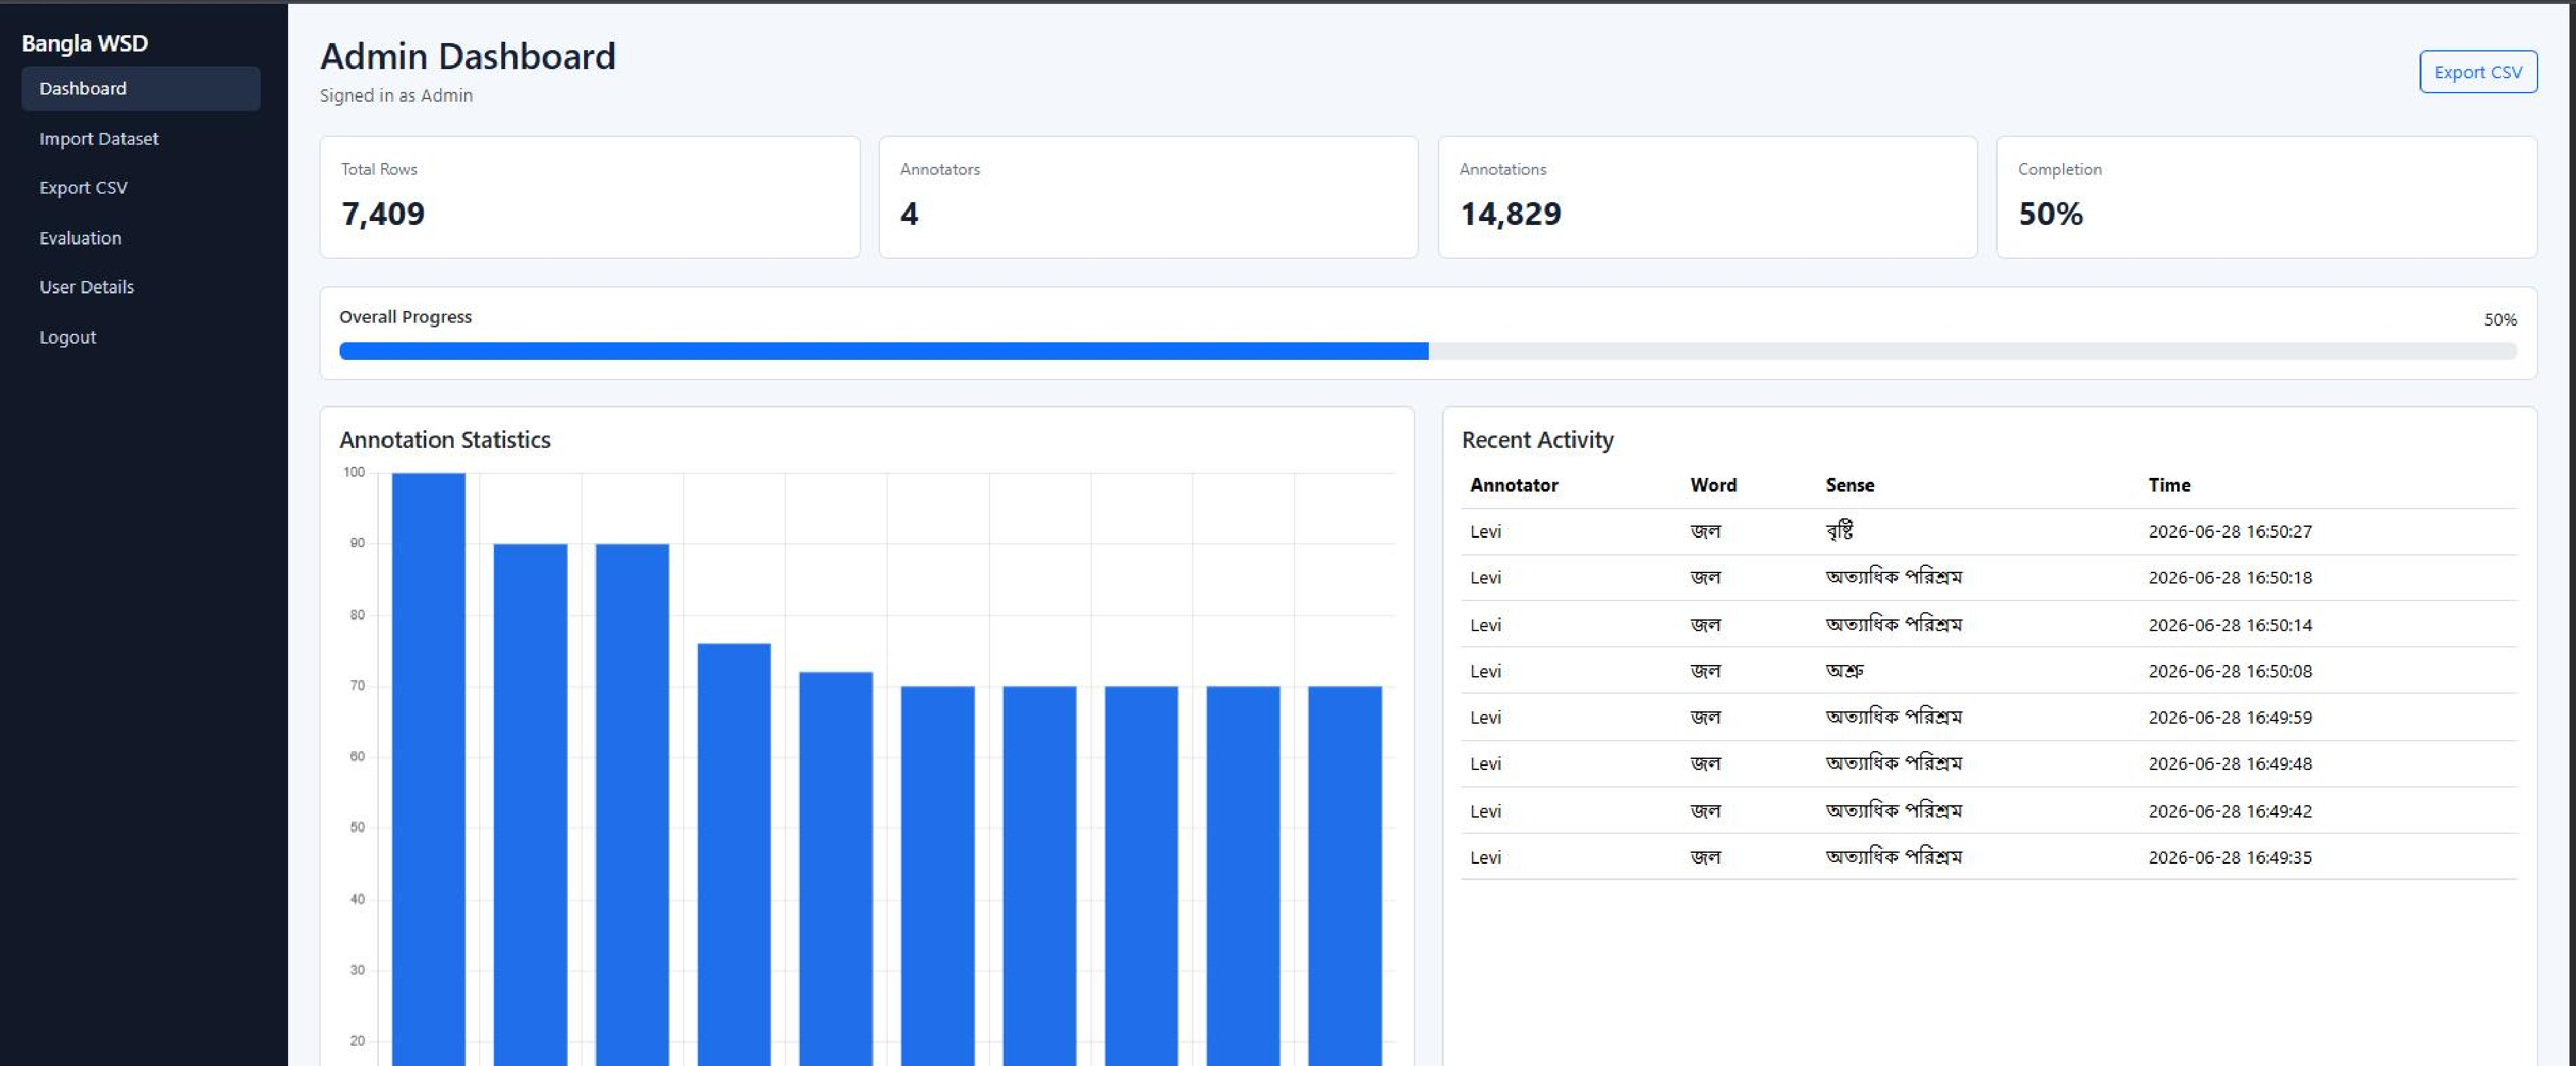
\includegraphics[width=0.92\textwidth]{website_images/annotation_admin_panel.pdf}
\caption{Administrator dashboard of the web annotation platform.}
\label{fig:annotation_admin_panel}
\end{figure}
\begin{figure}[htbp]
\centering
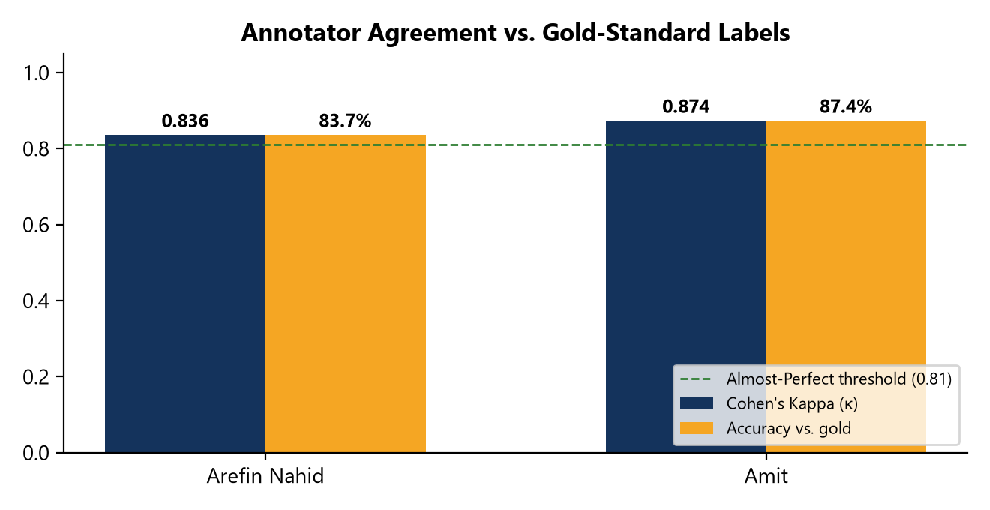
\includegraphics[width=0.72\textwidth]{details/figures/kappa_agreement_chart.pdf}
\caption{Cohen's Kappa and raw accuracy per annotator.}
\label{fig:kappa_chart}
\end{figure}
{\fontsize{12}{18}\selectfont\normalfont\setstretch{1.5}\justifying\sloppy\emergencystretch=3em
Applying Equation \ref{eq:kappa_pe} to each annotator's confusion matrix against the gold labels, raw agreement (\(p_o\)) is 83.7\% for Arefin Nahid and 87.4\% for Amit, only marginally above the corresponding \(\kappa\) values of 0.836 and 0.874; the small gap between \(p_o\) and \(\kappa\) in both cases indicates that the target words' sense distributions are only mildly skewed, so chance-level agreement \(p_e\) contributes little to the raw percentage, and the high measured agreement is attributable to genuine annotator consensus, not an artefact of one dominant sense per word. Both annotators clearing 0.80 independently (Figure 4.2), rather than only their average doing so, is the stronger reliability claim: it rules out the case where one careful and one careless annotator average out to an acceptable score.\par

}
\section{Full Benchmark Results (29 Experiments)}
{\fontsize{12}{18}\selectfont\normalfont\setstretch{1.5}\justifying\sloppy\emergencystretch=3em
Figure 4.3 plots test-set accuracy for all twenty-nine configurations, sorted descending. Fine-tuned BanglaBERT leads the ranking at 86.82\% accuracy, but it no longer leads it by a wide margin: frozen XLM-R target-span embeddings paired with plain logistic regression reach 86.37\%, and the top eight configurations, spanning fine-tuned, frozen-transformer, and even pretrained-fastText representations, all lie above 78\%. The strongest purely lexical baseline, TF-IDF + Linear SVM, reaches 64.89\%, roughly 22 points behind the leader. The clear message of the ranking is that representation quality, specifically, pretraining that covers Bangla, is what drives performance on this task: every configuration built on a pretrained Bangla-covering representation (fastText, XLM-R, mBERT, BanglaBERT) outperforms every configuration built on corpus-local TF-IDF statistics, and the single exception, XLM-R-FineTuned at 0.09\%, is a training failure analysed in Section 4.5, not a representation deficiency.\par

}
\begin{figure}[htbp]
\centering
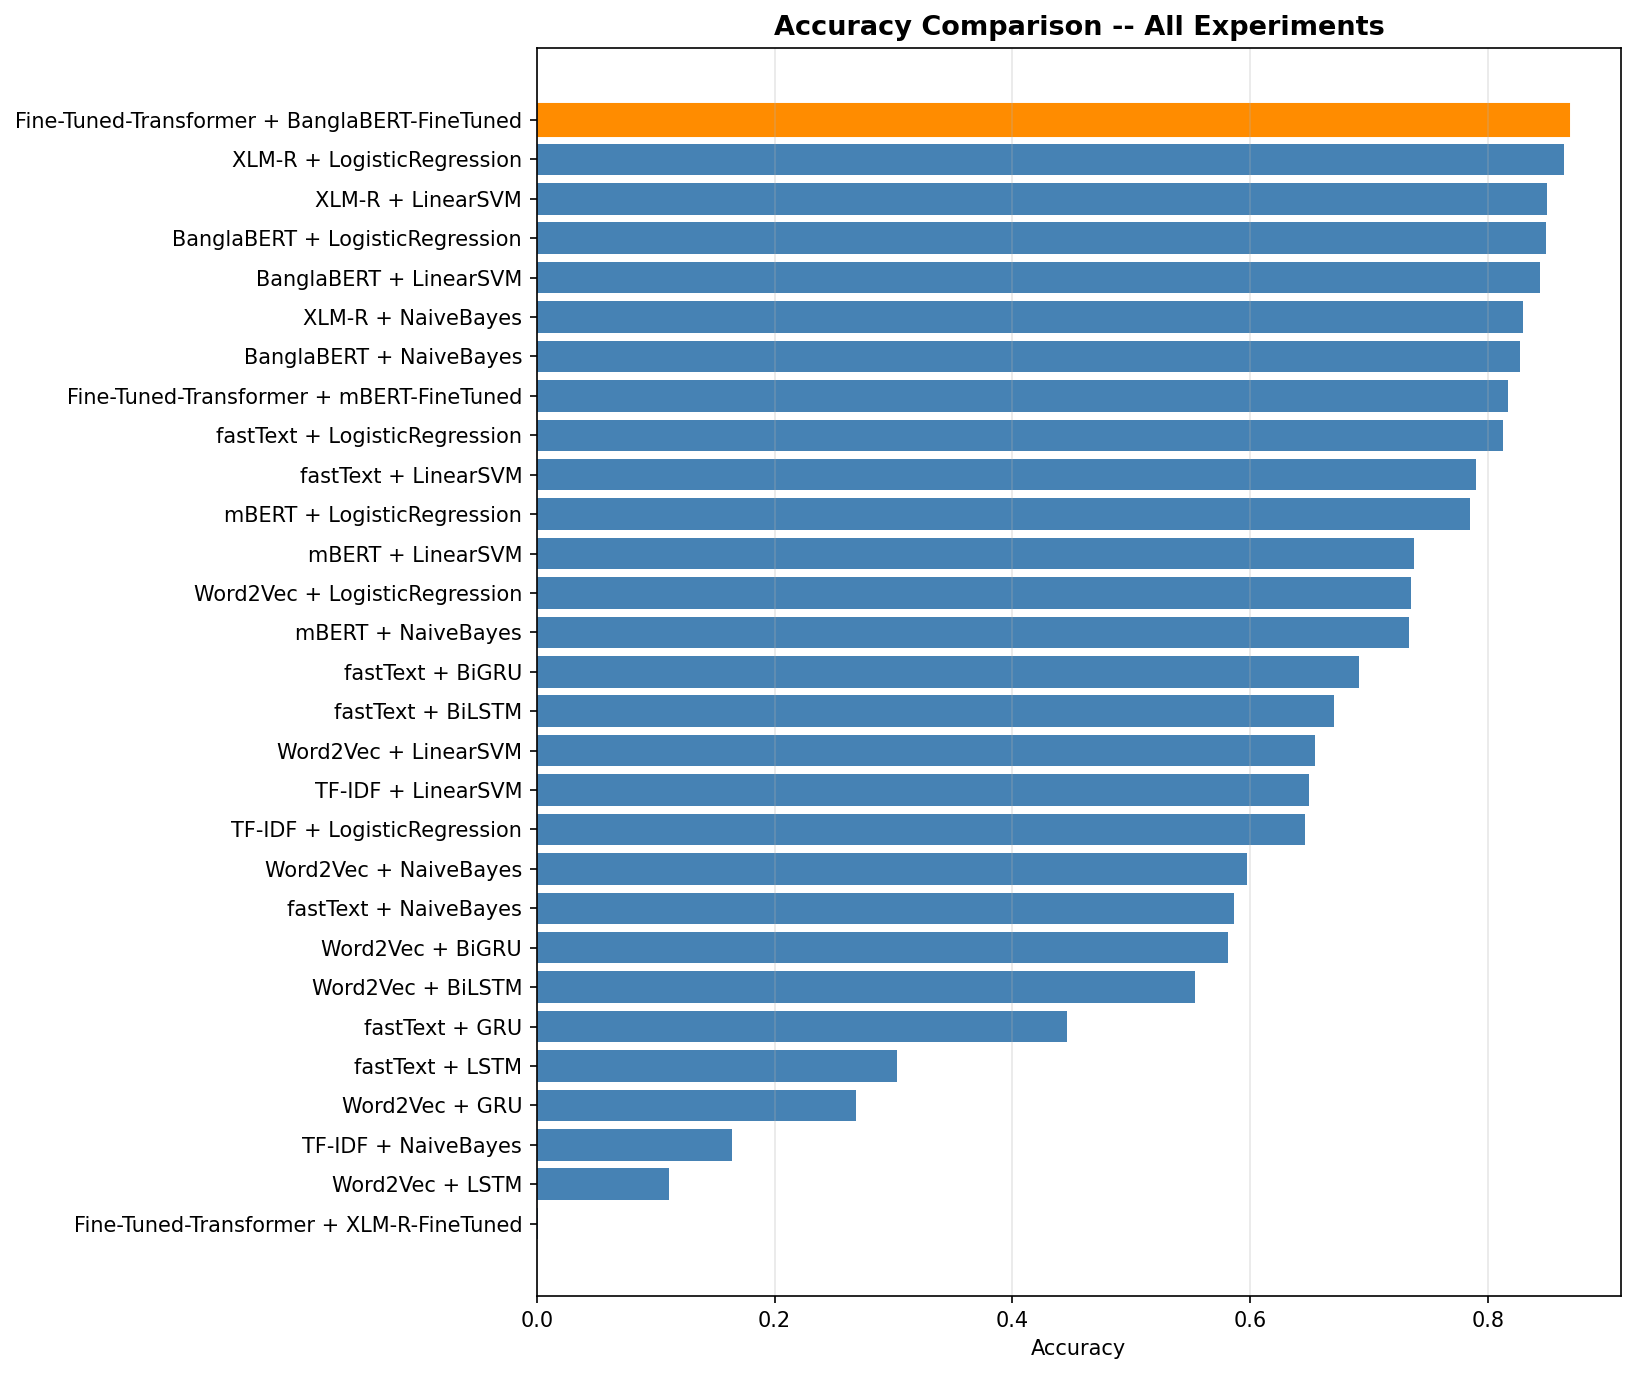
\includegraphics[width=0.8\textwidth]{figs_corrected/comparison_accuracy.png}
\caption{Test accuracy of all 29 experiments on the shared fixed split, sorted descending.}
\label{fig:auto1}
\end{figure}
{\fontsize{12}{18}\selectfont\normalfont\setstretch{1.5}\justifying\sloppy\emergencystretch=3em
Table 4.2 lists the top five configurations by macro F1, extracted from the notebook's results\_thesis\_table.docx export, with the failed XLM-R-FineTuned row appended for contrast.\par

}
\begin{table}[htbp]
\caption{Top five configurations by macro F1 on the shared fixed split, with the failed XLM-R fine-tuning run appended for contrast.}
\label{tab:auto15}
\centering
{\fontsize{9}{12}\selectfont
\setlength{\tabcolsep}{3pt}
\begin{tabular}{@{}p{4.20cm} p{2.35cm} p{2.35cm} p{2.35cm} p{2.35cm}@{}}
\toprule
\textbf{Embedding / Model} & \textbf{Accuracy} & \textbf{Precision} & \textbf{Recall} & \textbf{F1} \\
\midrule
BanglaBERT-FineTuned & 86.82\% & 85.66\% & 87.34\% & 85.00\% \\
\addlinespace[3pt]
XLM-R + Logistic Regression & 86.37\% & 84.46\% & 86.15\% & 83.78\% \\
\addlinespace[3pt]
BanglaBERT + Logistic Regression & 84.84\% & 83.39\% & 85.36\% & 82.71\% \\
\addlinespace[3pt]
XLM-R + Linear SVM & 84.93\% & 82.98\% & 84.63\% & 81.90\% \\
\addlinespace[3pt]
BanglaBERT + Linear SVM & 84.39\% & 82.42\% & 84.42\% & 81.52\% \\
\addlinespace[3pt]
XLM-R-FineTuned & 0.09\% & 0.00\% & 0.15\% & 0.00\% \\
\addlinespace[3pt]
\bottomrule
\end{tabular}}
\end{table}
{\fontsize{12}{18}\selectfont\normalfont\setstretch{1.5}\justifying\sloppy\emergencystretch=3em
Two aspects of Table 4.2 deserve emphasis. First, four of the five best configurations require no fine-tuning at all: a frozen transformer embedding plus a linear classifier, trainable in seconds on cached features, lands within 0.5--2.5 accuracy points of the fully fine-tuned leader. Second, XLM-R appears at both extremes of the ranking simultaneously, supplying the best frozen representation (86.37\% with logistic regression) while failing outright when fine-tuned end-to-end under the shared recipe, a paradox Section 4.5 examines in detail.\par

Table 4.3 reproduces the complete twenty-nine-row benchmark exported to results\_thesis\_table.docx (accuracy with macro-averaged precision, recall, and F1), so that every embedding/classifier combination, not only the top five of Table 4.2, is available for inspection.\par

}
\begin{center}
{\fontsize{8}{10}\selectfont
\setlength{\tabcolsep}{4pt}
\begin{longtable}{@{}p{2.55cm} p{2.55cm} p{1.85cm} p{1.85cm} p{1.85cm} p{1.85cm}@{}}
\caption{Full benchmark results for all 29 experiments on the shared fixed split (macro-averaged precision, recall, and F1).}\label{tab:full45}\\
\toprule
\textbf{Embedding} & \textbf{Model} & \textbf{Accuracy} & \textbf{Precision} & \textbf{Recall} & \textbf{F1-Score} \\
\midrule
\endfirsthead
\multicolumn{6}{l}{\textit{Table \ref{tab:full45} continued from previous page}}\\
\toprule
\textbf{Embedding} & \textbf{Model} & \textbf{Accuracy} & \textbf{Precision} & \textbf{Recall} & \textbf{F1-Score} \\
\midrule
\endhead
\midrule \multicolumn{6}{r}{\textit{continued on next page}}\\
\endfoot
\bottomrule
\endlastfoot
TF-IDF & Naive Bayes & 16.43\% & 10.86\% & 10.09\% & 9.79\% \\
TF-IDF & Logistic Regression & 64.62\% & 60.15\% & 64.54\% & 59.06\% \\
TF-IDF & Linear SVM & 64.89\% & 59.57\% & 63.92\% & 58.91\% \\
\midrule
Word2Vec & Naive Bayes & 59.75\% & 53.63\% & 59.25\% & 53.61\% \\
Word2Vec & Logistic Regression & 73.47\% & 69.87\% & 73.26\% & 69.21\% \\
Word2Vec & Linear SVM & 65.43\% & 59.53\% & 64.92\% & 59.23\% \\
Word2Vec & LSTM & 11.10\% & 8.05\% & 10.25\% & 8.03\% \\
Word2Vec & GRU & 26.81\% & 19.14\% & 23.89\% & 19.58\% \\
Word2Vec & BiLSTM & 55.32\% & 50.16\% & 54.73\% & 49.48\% \\
Word2Vec & BiGRU & 58.12\% & 51.37\% & 56.44\% & 50.72\% \\
\midrule
fastText & Naive Bayes & 58.66\% & 52.79\% & 58.41\% & 52.45\% \\
fastText & Logistic Regression & 81.23\% & 79.47\% & 81.79\% & 78.45\% \\
fastText & Linear SVM & 78.97\% & 75.26\% & 78.79\% & 74.67\% \\
fastText & LSTM & 30.32\% & 23.89\% & 29.12\% & 23.89\% \\
fastText & GRU & 44.58\% & 38.43\% & 43.20\% & 37.66\% \\
fastText & BiLSTM & 67.06\% & 61.87\% & 66.06\% & 60.66\% \\
fastText & BiGRU & 69.13\% & 63.39\% & 67.74\% & 62.58\% \\
\midrule
XLM-R & Naive Bayes & 82.94\% & 79.38\% & 82.34\% & 78.92\% \\
XLM-R & Logistic Regression & 86.37\% & 84.46\% & 86.15\% & 83.78\% \\
XLM-R & Linear SVM & 84.93\% & 82.98\% & 84.63\% & 81.90\% \\
\midrule
mBERT & Naive Bayes & 73.38\% & 69.70\% & 72.80\% & 68.77\% \\
mBERT & Logistic Regression & 78.43\% & 75.02\% & 78.10\% & 74.47\% \\
mBERT & Linear SVM & 73.74\% & 69.71\% & 73.36\% & 69.23\% \\
\midrule
BanglaBERT & Naive Bayes & 82.67\% & 79.91\% & 81.94\% & 79.04\% \\
BanglaBERT & Logistic Regression & 84.84\% & 83.39\% & 85.36\% & 82.71\% \\
BanglaBERT & Linear SVM & 84.39\% & 82.42\% & 84.42\% & 81.52\% \\
\midrule
BanglaBERT & Fine-Tuned & 86.82\% & 85.66\% & 87.34\% & 85.00\% \\
mBERT & Fine-Tuned & 81.68\% & 78.48\% & 81.27\% & 77.83\% \\
XLM-R & Fine-Tuned & 0.09\% & 0.00\% & 0.15\% & 0.00\% \\
\end{longtable}}
\end{center}
{\fontsize{12}{18}\selectfont\normalfont\setstretch{1.5}\justifying\sloppy\emergencystretch=3em
Figure 4.4 re-plots the same twenty-nine experiments by macro F1, the metric least forgiving of rare-sense neglect, and Figure 4.5 summarises accuracy alongside macro- and weighted-averaged precision, recall, and F1 for every experiment in a single heatmap, so that the patterns discussed below can be verified across all metrics at once rather than on accuracy alone. Three within-embedding patterns stand out. First, logistic regression is the strongest classical learner on every embedding except TF-IDF (where Linear SVM edges it by 0.27 points), and on the frozen transformer embeddings even Naive Bayes exceeds 82\% (XLM-R 82.94\%, BanglaBERT 82.67\%): the target-span representations are linearly separable enough that classifier choice matters far less than representation choice. Second, TF-IDF + Naive Bayes collapses to 16.43\% while logistic regression and Linear SVM handle the same 30,000-dimensional sparse bigram space at close to 65\%, so the collapse is attributable to Naive Bayes's independence assumption breaking down over correlated n-gram features spread across 657 classes, not to the representation itself. Third, among the recurrent architectures the bidirectional variants dominate their unidirectional counterparts on both sequence-capable embeddings (Word2Vec: BiGRU 58.12\% versus GRU 26.81\% and LSTM 11.10\%; fastText: BiGRU 69.13\% versus GRU 44.58\% and LSTM 30.32\%), yet even the best recurrent model remains 12--15 points behind plain logistic regression on the target-aware pooled features of the same embedding. With only 5,166 training sentences spread over 657 classes, a recurrent encoder has too little data to out-learn a linear model that is already handed a target-focused representation.\par

}
\begin{figure}[htbp]
\centering
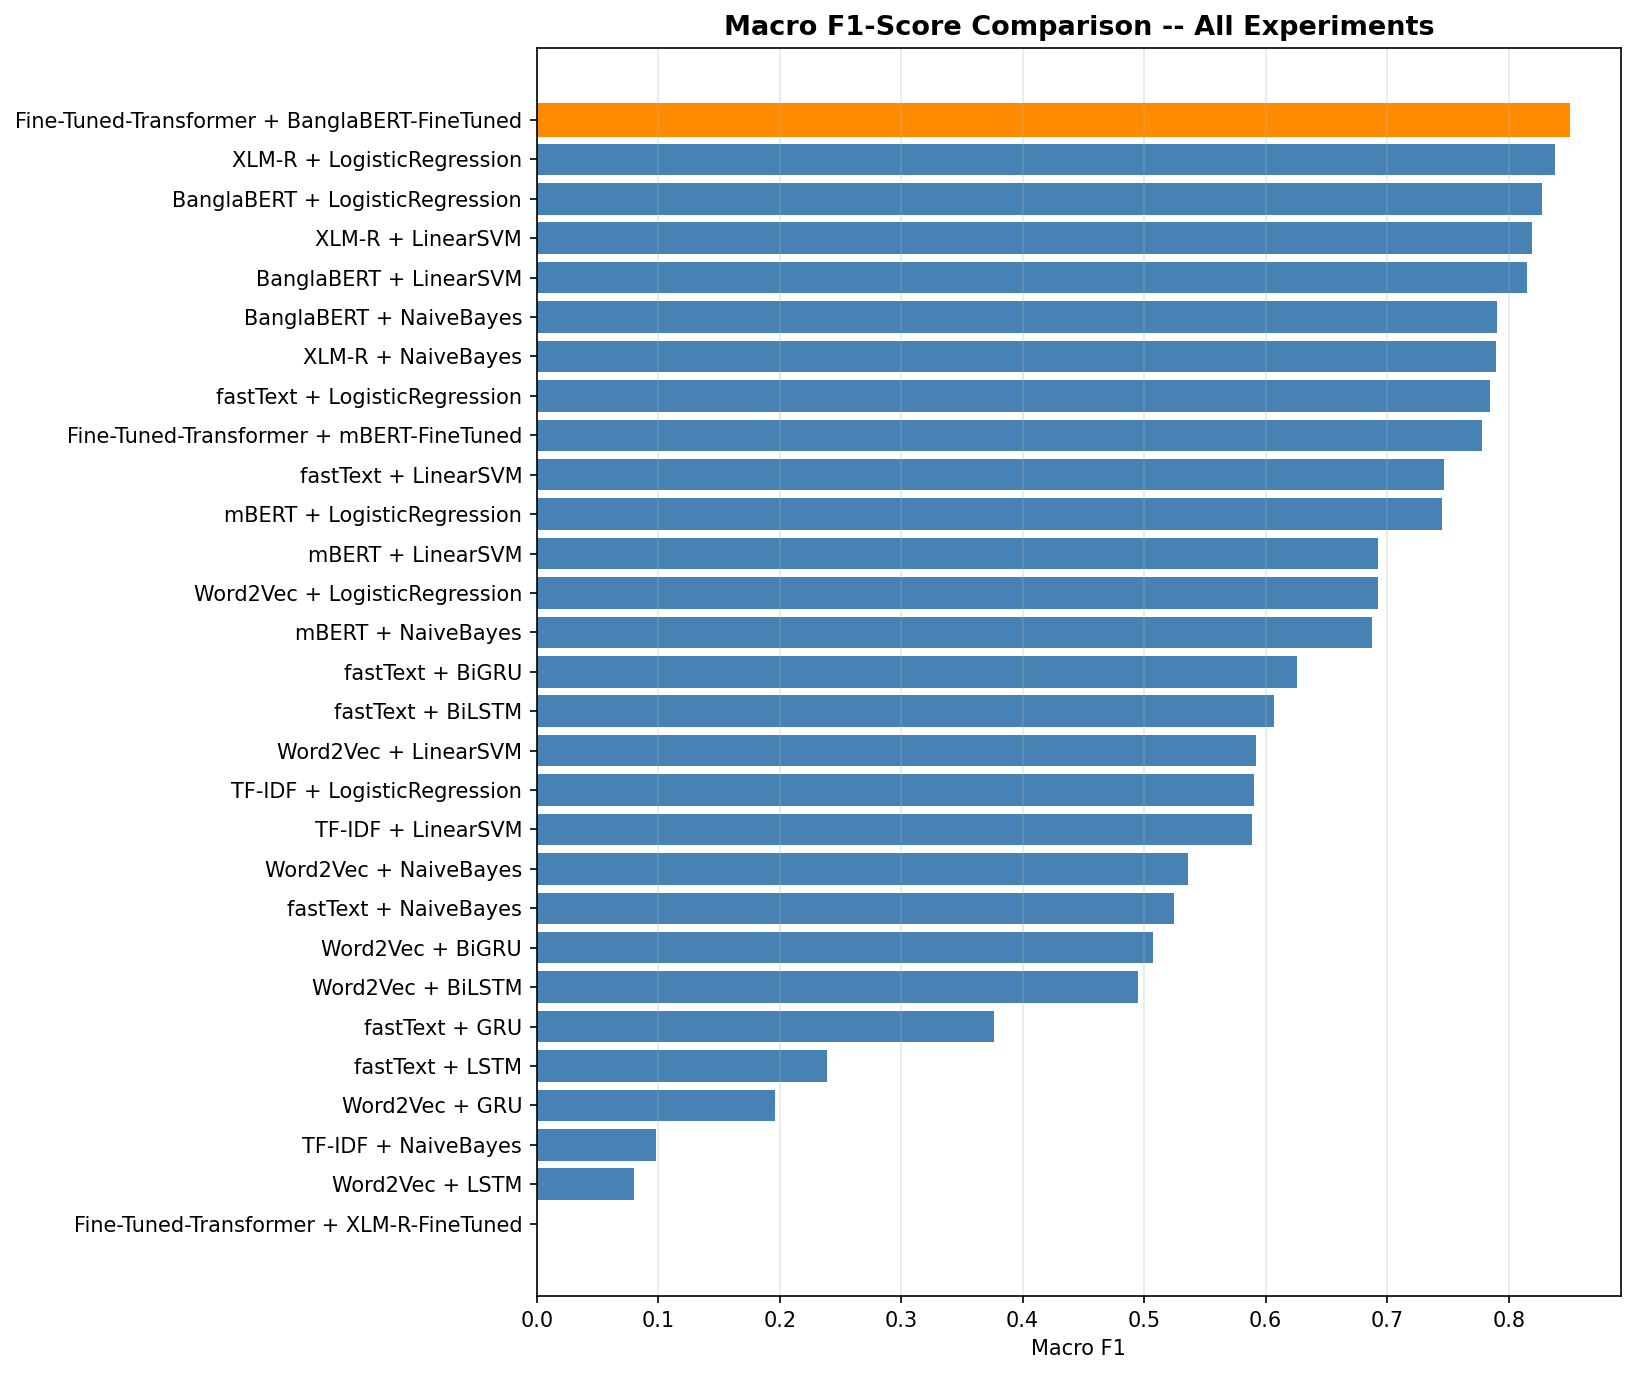
\includegraphics[width=0.8\textwidth]{figs_corrected/comparison_macro_f1.png}
\caption{Macro F1 of all 29 experiments on the shared fixed split, sorted descending.}
\label{fig:macro_f1_bar}
\end{figure}
\begin{figure}[htbp]
\centering
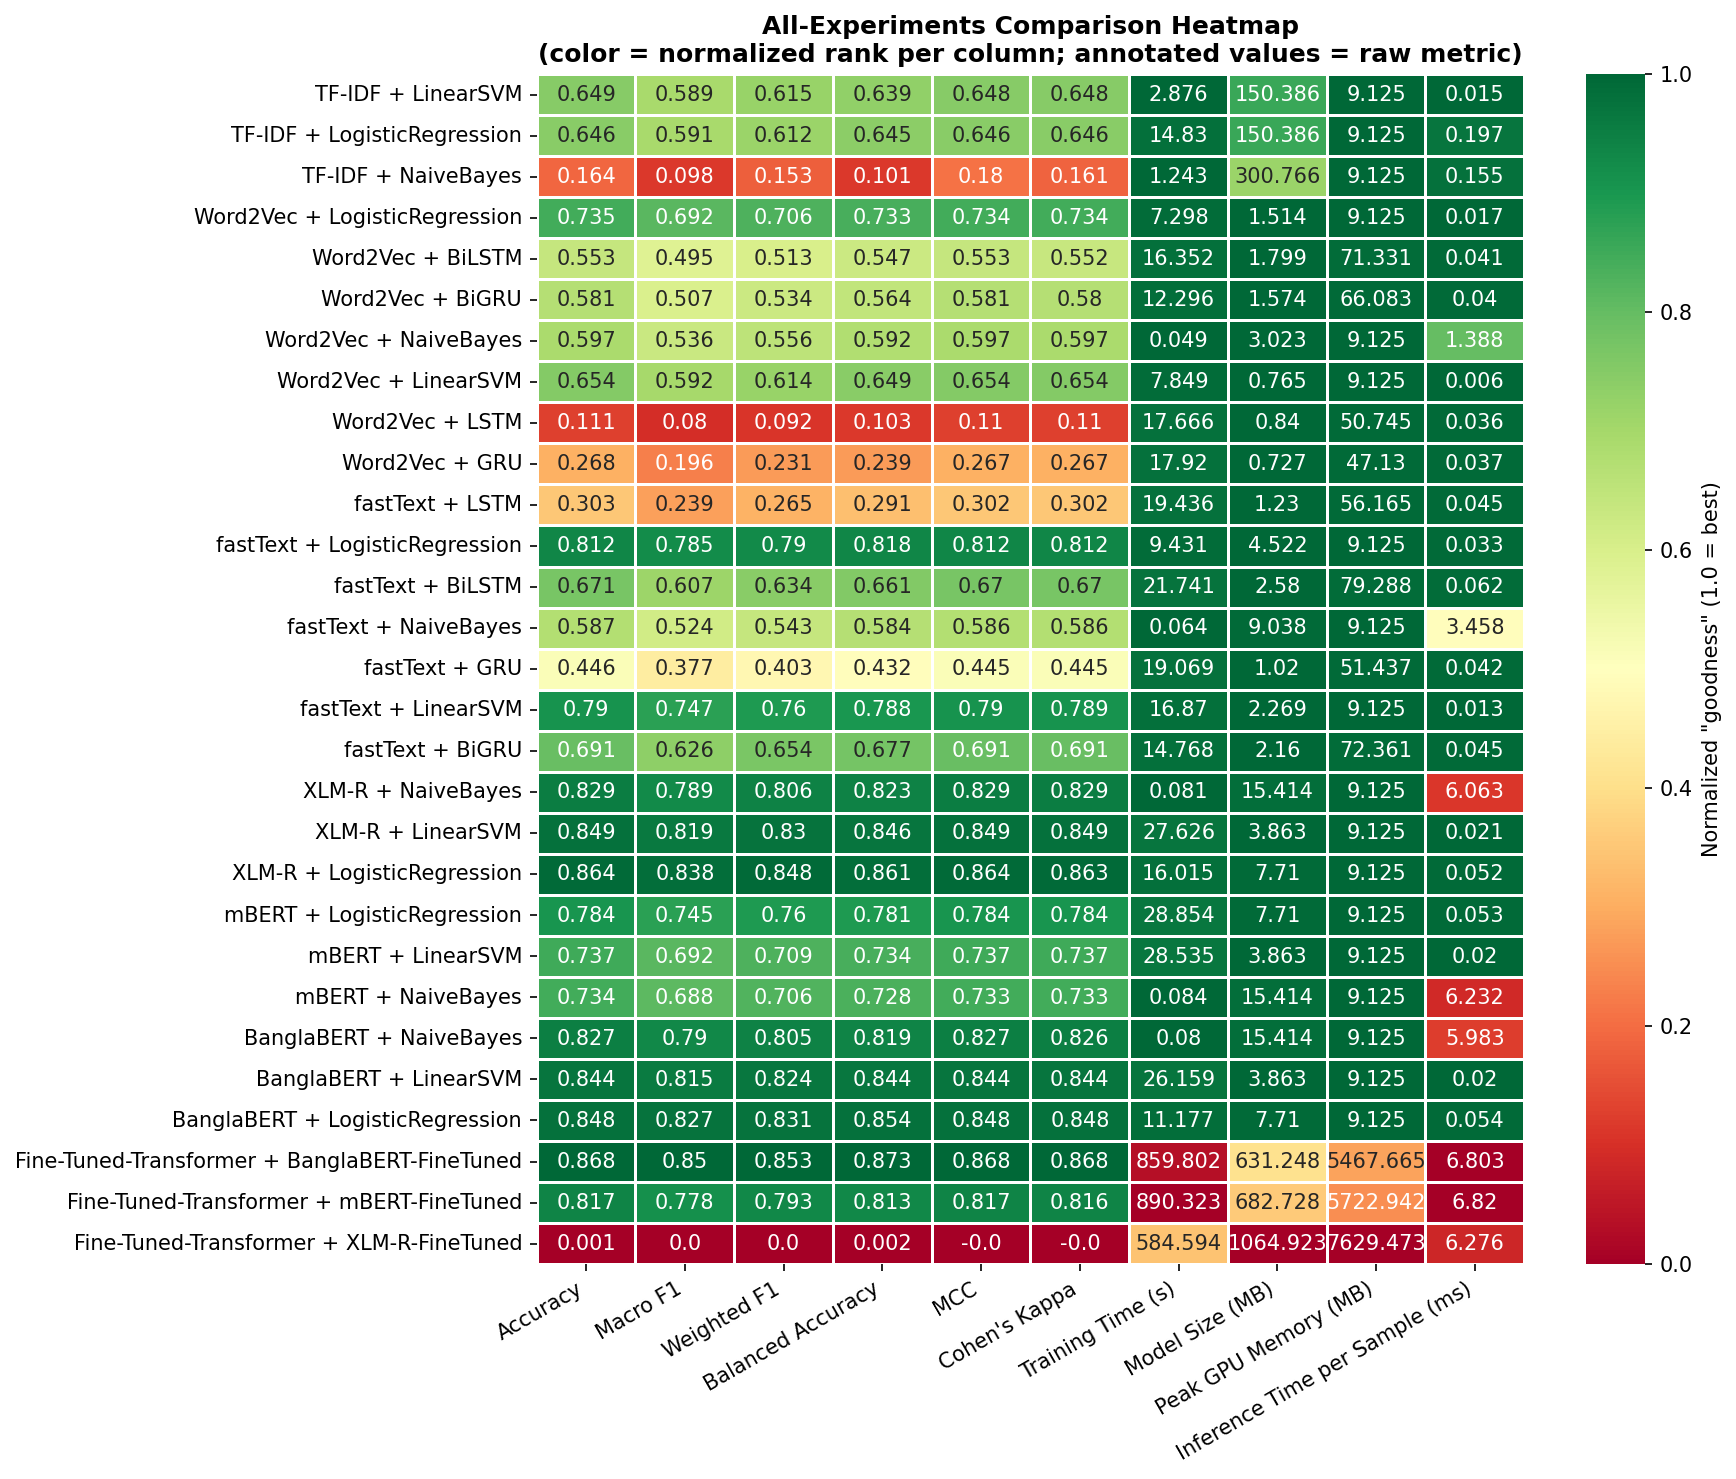
\includegraphics[width=0.95\textwidth]{figs_corrected/comparison_heatmap_all_metrics.png}
\caption{Heatmap of accuracy and macro/weighted precision, recall, and F1 for all 29 experiments, embeddings and classifiers as rows, metrics as columns.}
\label{fig:metrics_heatmap}
\end{figure}
\section{Fine-Tuned Transformer Results}
{\fontsize{12}{18}\selectfont\normalfont\setstretch{1.5}\justifying\sloppy\emergencystretch=3em
Table 4.4 reports the three end-to-end fine-tuning experiments on the same fixed split used by every other experiment: the best validation accuracy reached (and the epoch it was reached at), together with test accuracy and macro-averaged precision, recall, and F1. BanglaBERT-FineTuned converges smoothly, its validation accuracy climbing from 12.38\% after the first epoch to a best of 88.80\% at epoch 13, and generalises to 86.82\% test accuracy. mBERT-FineTuned follows the same trajectory more slowly, still improving at the epoch-15 budget cap (best validation 83.20\% at epoch 15), and reaches 81.68\% on test. XLM-R-FineTuned never leaves the random-guessing floor: its validation accuracy peaks at 0.18\% and early stopping abandons training at epoch 8.\par

}
\begin{table}[htbp]
\caption{Fine-tuning results on the shared fixed split: best validation accuracy with the epoch it occurred at, and held-out test metrics (macro-averaged).}
\label{tab:auto16}
\centering
{\fontsize{8}{9.5}\selectfont
\setlength{\tabcolsep}{3pt}
\begin{tabular}{@{}p{3.15cm} p{2.30cm} p{1.75cm} p{1.85cm} p{1.75cm} p{1.65cm}@{}}
\toprule
\textbf{Model} & \textbf{Best Val.\ Acc.\ (epoch)} & \textbf{Test Accuracy} & \textbf{Macro Prec.} & \textbf{Macro Rec.} & \textbf{Macro F1} \\
\midrule
BanglaBERT-FineTuned & 88.80\% (13) & 86.82\% & 85.66\% & 87.34\% & 85.00\% \\
\addlinespace[3pt]
mBERT-FineTuned & 83.20\% (15) & 81.68\% & 78.48\% & 81.27\% & 77.83\% \\
\addlinespace[3pt]
XLM-R-FineTuned & 0.18\% (4; stopped at 8) & 0.09\% & 0.00\% & 0.15\% & 0.00\% \\
\addlinespace[3pt]
\bottomrule
\end{tabular}}
\end{table}
{\fontsize{12}{18}\selectfont\normalfont\setstretch{1.5}\justifying\sloppy\emergencystretch=3em
Fine-tuned BanglaBERT outperforms fine-tuned mBERT by 5.1 accuracy points and 7.2 macro-F1 points under a byte-for-byte identical recipe, which is the first controlled evidence among the studies reviewed in Chapter 2 that Bangla-specific pretraining measurably outperforms general-purpose multilingual pretraining on Bangla WSD once both are fine-tuned under shared conditions. Equally instructive is how narrow the margin over the frozen alternative has become: BanglaBERT-FineTuned's 86.82\%/85.00\% exceeds frozen XLM-R + Logistic Regression (86.37\%/83.78\%, Table 4.2) by only 0.45 accuracy points and 1.22 macro-F1 points, while costing roughly 860 seconds of GPU fine-tuning against about 16 seconds of classifier training on cached embeddings (plus a one-off 38-second embedding-generation pass), and 6.8 ms per prediction against 0.05 ms. Fine-tuning still buys the best result, but with target-aware frozen features the gap is no longer the order-of-magnitude chasm that motivates fine-tuning unconditionally; for deployments where GPU fine-tuning is infeasible, a frozen-embedding pipeline is now a defensible alternative. Model size and inference cost (Table 4.5) also favour BanglaBERT among the fine-tuned models: it is the smallest of the three and the most accurate.\par

}
\begin{table}[htbp]
\caption{Fine-tuned model size, parameters, and inference cost on the shared fixed split.}
\label{tab:auto17}
\centering
{\fontsize{9}{12}\selectfont
\setlength{\tabcolsep}{3pt}
\begin{tabular}{@{}p{1.90cm} p{3.09cm} p{3.09cm} p{3.09cm} p{3.09cm}@{}}
\toprule
\textbf{Model} & \textbf{Parameters} & \textbf{Model Size} & \textbf{Inference / Sample} & \textbf{ROC-AUC (macro)} \\
\midrule
BanglaBERT-FineTuned & 165.5M & 631.2 MB & 6.80 ms & 99.99\% \\
\addlinespace[3pt]
mBERT-FineTuned & 179.0M & 682.7 MB & 6.82 ms & 99.97\% \\
\addlinespace[3pt]
XLM-R-FineTuned & 279.1M & 1,064.9 MB & 6.28 ms & 51.79\% (chance level) \\
\addlinespace[3pt]
\bottomrule
\end{tabular}}
\end{table}
{\fontsize{12}{18}\selectfont\normalfont\setstretch{1.5}\justifying\sloppy\emergencystretch=3em

\subsection{The XLM-R Negative Result}

XLM-R-FineTuned's near-chance macro ROC-AUC (51.79\%, against 99.97--99.99\% for the other two backbones) indicates outright training failure rather than a merely weaker fit. Figures 4.6--4.7 compare the training curves of BanglaBERT-FineTuned and XLM-R-FineTuned: BanglaBERT's training loss falls from 6.47 to near zero within 15 epochs while validation accuracy rises to 88.80\%, whereas XLM-R's loss plateaus near \(\ln(657) \approx 6.49\), the loss of uniform random guessing over 657 classes, and validation accuracy never exceeds 0.18\% before early stopping halts training at epoch 8.\par

The failure was investigated systematically rather than merely reported. The initial hypothesis was tokenizer-specific: XLM-R's SentencePiece tokenizer fragments the literal string ``[TGT]'' into four context-dependent sub-word pieces (and ``[/TGT]'' into five), destroying the marker's value as a stable attention anchor, whereas the WordPiece tokenizers of mBERT and BanglaBERT split the same brackets more consistently. The corrected pipeline therefore registers both markers as atomic special tokens for every backbone (Section 3.6); a pre-training diagnostic confirms that after registration each marker maps to exactly one stable token id (250002 and 250003 for XLM-R), that the label space is consistent (label ids 0--656 against a 657-way classifier head), and that a forward--backward smoke test delivers non-zero gradients into the backbone, ruling out an accidentally frozen encoder. Yet the failure persists under the fix: with an atomic [TGT] signal, verified labels, and verified gradient flow, XLM-R still cannot escape the random-guessing plateau under the recipe that carries mBERT and BanglaBERT past 80\%. What remains is a genuine backbone-specific optimisation failure: XLM-R is the largest of the three models (279M parameters, most of them in its 250,000-row embedding matrix), and the shared learning-rate and warm-up budget that suits the two BERT-family backbones appears simply too conservative to move it off its initialisation within the epoch budget. The paradox sharpened by Table 4.2 is that the same frozen backbone supplies the single best non-fine-tuned representation in the benchmark (86.37\% with logistic regression): the pretrained representation is excellent; it is the shared fine-tuning recipe that fails it. This negative result is documented here, and it is what causes the live demo application (Section 4.8) to exclude XLM-R-FineTuned automatically.\par

}
\begin{figure}[htbp]
\centering
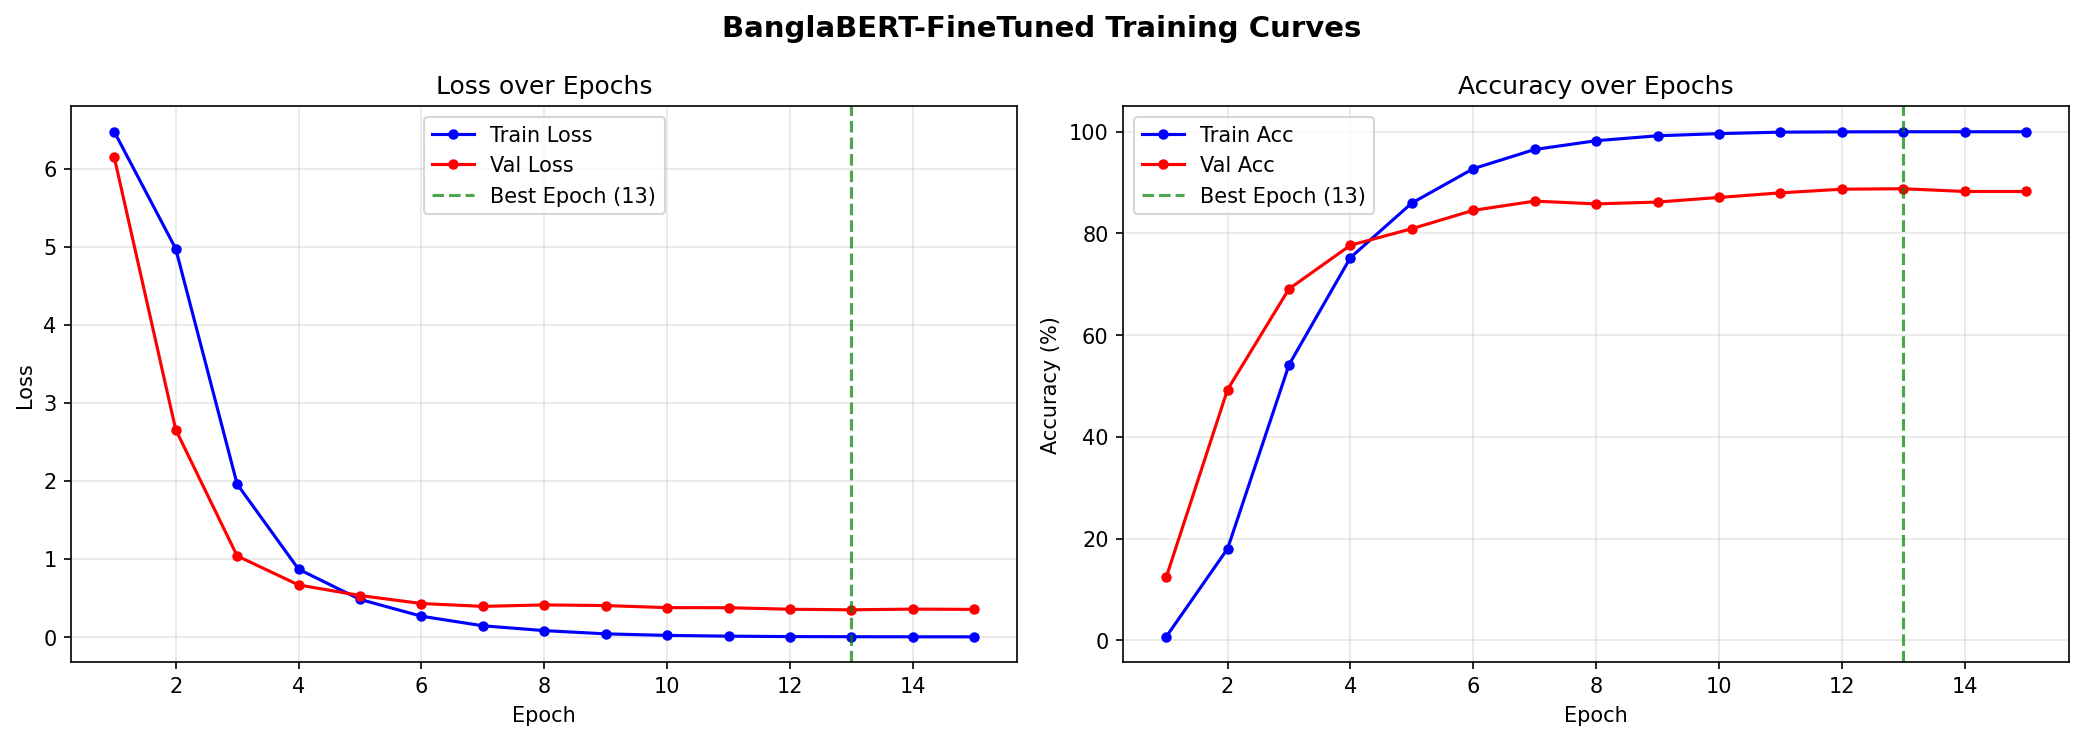
\includegraphics[width=0.8\textwidth]{figs_corrected/BanglaBERT-FineTuned_training_curves.png}
\caption{Training curves of BanglaBERT-FineTuned: loss falls to near zero while validation accuracy climbs to 88.80\%.}
\label{fig:auto2}
\end{figure}
{\fontsize{12}{18}\selectfont\normalfont\setstretch{1.5}\justifying\sloppy\emergencystretch=3em
}
\begin{figure}[htbp]
\centering
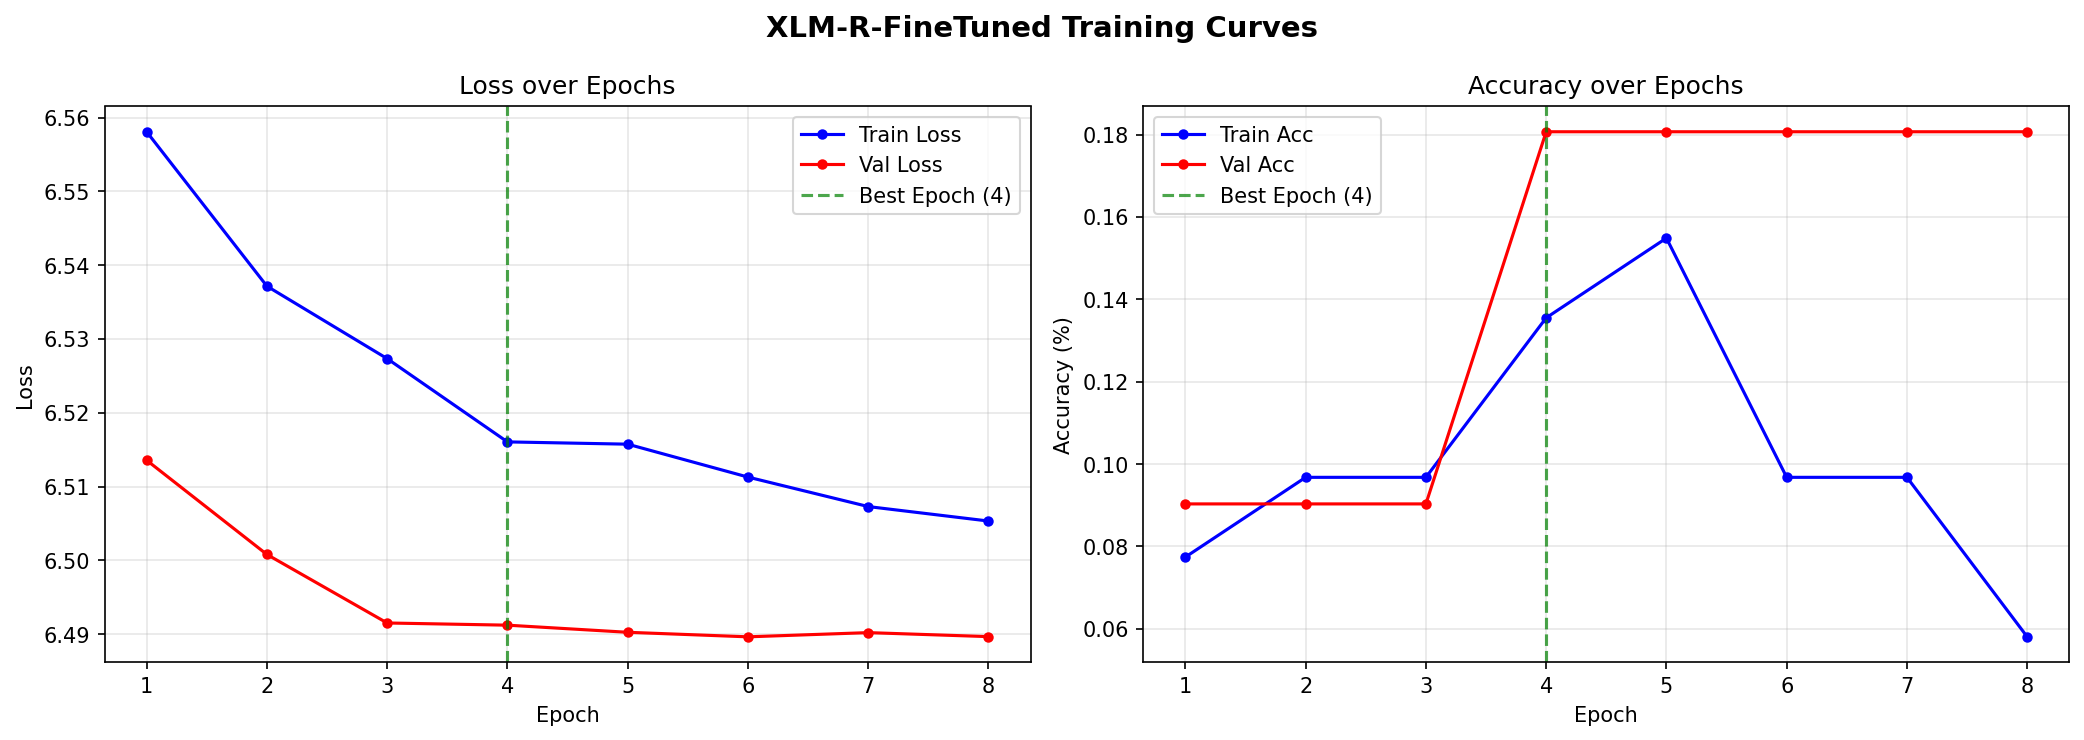
\includegraphics[width=0.8\textwidth]{figs_corrected/XLM-R-FineTuned_training_curves.png}
\caption{Training curves of XLM-R-FineTuned: loss plateaus at the 657-class random-guessing level (\(\ln 657 \approx 6.49\)) and validation accuracy never exceeds 0.18\%.}
\label{fig:auto3}
\end{figure}
{\fontsize{12}{18}\selectfont\normalfont\setstretch{1.5}\justifying\sloppy\emergencystretch=3em
}
\section{Error Analysis}
{\fontsize{12}{18}\selectfont\normalfont\setstretch{1.5}\justifying\sloppy\emergencystretch=3em
On the 1,108-sentence test set, BanglaBERT-FineTuned misclassifies 146 sentences (13.18\% error rate) and mBERT-FineTuned misclassifies 203 (18.32\%). The decisive structural finding comes from decomposing those errors by target word: 145 of BanglaBERT-FineTuned's 146 errors (99.3\%), and 202 of mBERT-FineTuned's 203 (99.5\%), are \emph{within-word} confusions, the model choosing a wrong sense of the correct target word, with exactly one cross-word error apiece. The 657-way global classifier has, in effect, already learned to identify which word is being disambiguated; essentially all residual difficulty lies in separating semantically adjacent senses of the same word. Table 4.6 lists the most frequently confused sense pairs for BanglaBERT-FineTuned, extracted directly from the model's confusion matrix.\par

Both models' confusion matrices are dominated by their diagonal, confirming that neither model fails broadly across the 657-class space; the difference between them is one of degree, a modestly thicker band of off-diagonal mass for mBERT-FineTuned, rather than a qualitatively different error pattern. This is the confusion-matrix-level evidence for the same conclusion Section 4.5 reaches from the accuracy numbers: Bangla-specific pretraining reduces errors broadly across the sense space; the gain does not come from fixing a handful of specific senses.\par

}
\begin{table}[htbp]
\caption{Most frequently confused sense pairs, BanglaBERT-FineTuned (test set).}
\label{tab:auto18}
\centering
{\fontsize{10}{14}\selectfont
\begin{tabular}{@{}>{\raggedright\arraybackslash}p{6.10cm} >{\raggedright\arraybackslash}p{6.10cm} >{\centering\arraybackslash}p{1.60cm}@{}}
\toprule
\textbf{Gold Sense} & \textbf{Predicted As} & \textbf{Count} \\
\midrule
\bn{রূপ: আকৃতি} (shape) & \bn{রূপ: সৌন্দর্য} (beauty) & 2 \\
\addlinespace[3pt]
\bn{রেখা: চিহ্ন} (mark) & \bn{রেখা: দাগ বা লাইন} (line) & 2 \\
\addlinespace[3pt]
\bn{বিষয়: মামলা-মকদ্দমা} (lawsuit) & \bn{বিষয়: সমস্যা} (problem) & 2 \\
\addlinespace[3pt]
\bn{রস: স্বাদ} (taste) & \bn{রস: তরল নির্যাস} (liquid extract) & 2 \\
\addlinespace[3pt]
\bn{কলি: ফুলের কুঁড়ি} (flower bud) & \bn{কলি: অঙ্কুর} (sprout) & 2 \\
\addlinespace[3pt]
\bn{কক্ষ: ঘর} (room) & \bn{কক্ষ: শ্রেণিকক্ষ} (classroom) & 2 \\
\addlinespace[3pt]
\bottomrule
\end{tabular}}
\end{table}
{\fontsize{12}{18}\selectfont\normalfont\setstretch{1.5}\justifying\sloppy\emergencystretch=3em
Every confusion in Table 4.6 occurs between two senses of the same target word, never between unrelated words, and every pair is semantically adjacent: shape versus beauty, mark versus line, flower bud versus sprout, room versus classroom. These are exactly the distinctions on which even careful human annotators would deliberate, and the confused senses are typically supported by only ten to twenty examples in the corpus, so the model receives the least evidence precisely for the senses that are hardest to separate from a closely related sibling. No confusion pair occurs more than twice, confirming that the residual error mass is spread thinly across many hard sense pairs rather than concentrated in a few systematically broken classes.\par

}
\section{Global versus Target-Word-Constrained Evaluation}
{\fontsize{12}{18}\selectfont\normalfont\setstretch{1.5}\justifying\sloppy\emergencystretch=3em
Every experiment was additionally evaluated under the target-word-constrained inference of Equation \ref{eq:constrained}, which restricts each prediction to the candidate senses of the known target word without retraining anything. Figure 4.8 plots global against constrained weighted F1 for all twenty-nine experiments, and Table 4.7 extracts representative rows. The pattern is sharply bimodal. Weak configurations gain enormously: TF-IDF + Naive Bayes jumps from 16.43\% to 70.31\% accuracy, and Word2Vec + LSTM from 11.10\% to 56.68\%, because most of their global errors are \emph{cross-word}, predictions of senses belonging to entirely different words, which the restriction eliminates wholesale. Strong configurations gain almost nothing: BanglaBERT-FineTuned improves only from 86.82\% to 86.91\% and frozen XLM-R + Logistic Regression from 86.37\% to 86.73\%, direct corroboration of Section 4.6's finding that over 99\% of a strong model's errors already lie \emph{within} the correct word's own sense set, where the restriction cannot help.\par

}
\begin{figure}[htbp]
\centering
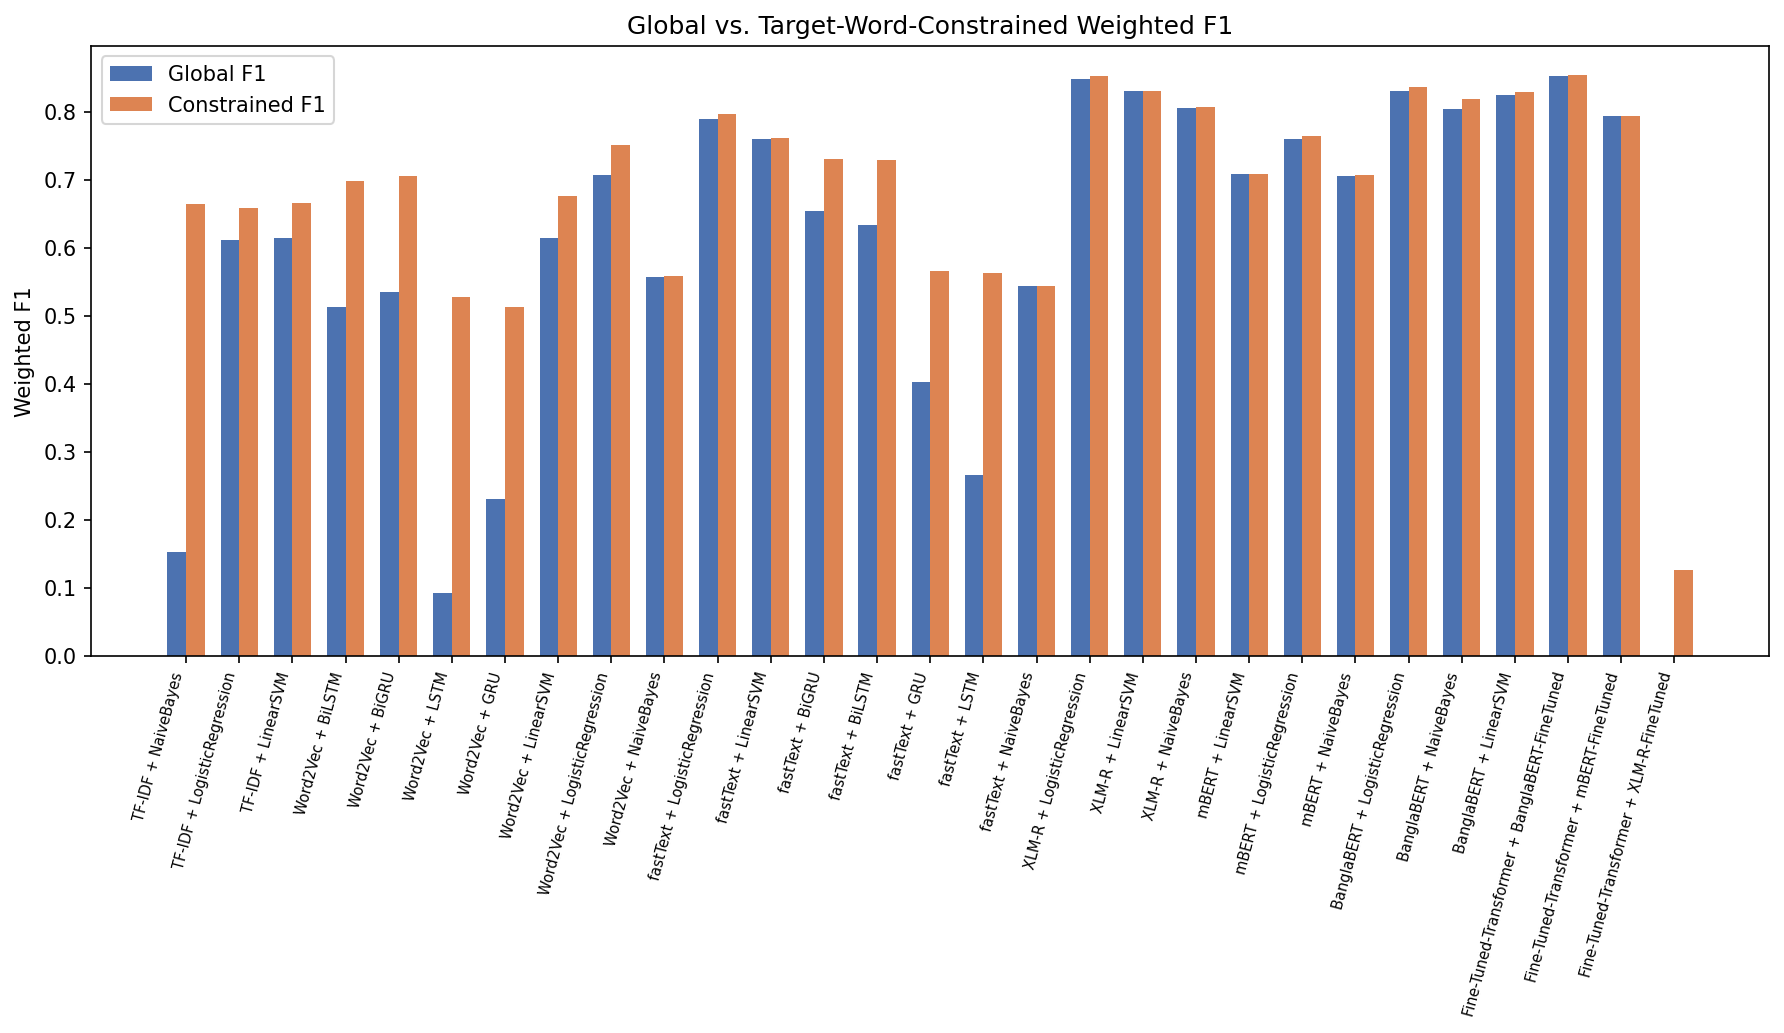
\includegraphics[width=0.8\textwidth]{figs_corrected/global_vs_constrained_f1.png}
\caption{Global versus target-word-constrained weighted F1 for all 29 experiments: weak configurations gain dramatically from the restriction while strong configurations are nearly unchanged.}
\label{fig:global_constrained}
\end{figure}
\begin{table}[htbp]
\caption{Representative global versus target-word-constrained test results (accuracy and weighted F1).}
\label{tab:global_constrained}
\centering
{\fontsize{9}{12}\selectfont
\setlength{\tabcolsep}{3pt}
\begin{tabular}{@{}p{4.60cm} p{2.20cm} p{2.20cm} p{2.40cm} p{2.40cm}@{}}
\toprule
\textbf{Configuration} & \textbf{Global Acc.} & \textbf{Global F1} & \textbf{Constr.\ Acc.} & \textbf{Constr.\ F1} \\
\midrule
TF-IDF + Naive Bayes & 16.43\% & 15.26\% & 70.31\% & 66.39\% \\
\addlinespace[3pt]
Word2Vec + LSTM & 11.10\% & 9.20\% & 56.68\% & 52.81\% \\
\addlinespace[3pt]
fastText + Logistic Regression & 81.23\% & 79.00\% & 81.77\% & 79.63\% \\
\addlinespace[3pt]
XLM-R + Logistic Regression & 86.37\% & 84.80\% & 86.73\% & 85.23\% \\
\addlinespace[3pt]
BanglaBERT-FineTuned & 86.82\% & 85.27\% & 86.91\% & 85.40\% \\
\addlinespace[3pt]
XLM-R-FineTuned & 0.09\% & 0.00\% & 27.53\% & 12.63\% \\
\addlinespace[3pt]
\bottomrule
\end{tabular}}
\end{table}
{\fontsize{12}{18}\selectfont\normalfont\setstretch{1.5}\justifying\sloppy\emergencystretch=3em
Two further readings of Table 4.7 matter. First, even under constrained inference the ranking of configurations is preserved, so the restriction is a deployment aid, not a substitute for a good model: XLM-R-FineTuned recovers only 27.53\% accuracy when constrained, barely above what guessing among a word's three-to-four candidate senses would yield, confirming that no inference-time trick rescues a model that learned nothing. Second, ranking quality reinforces the same picture: both successful fine-tuned models achieve near-perfect macro ROC-AUC (99.99\% BanglaBERT, 99.97\% mBERT; Table 4.5), meaning the correct sense is ranked at or near the top of the 657-way candidate list even on the sentences the model ultimately answers incorrectly, so most residual errors are narrow top-2 confusions between adjacent senses rather than confident, wide misses. This is why the live demo's sense-restricted confidence score (Section 3.11) remains a useful signal even on erroneous predictions.\par

}
\section{Live Demo Application}
{\fontsize{12}{18}\selectfont\normalfont\setstretch{1.5}\justifying\sloppy\emergencystretch=3em
The Gradio application described in Section 3.11 loads results.csv at start-up and automatically ranks the three fine-tuned models by test accuracy; since XLM-R-FineTuned's 0.09\% accuracy places it last, the application serves only BanglaBERT-FineTuned and mBERT-FineTuned side by side, without any hard-coded exclusion list. Given a sentence and a target word, both models produce a sense-restricted prediction, a confidence score, and per-model latency, alongside a Benchmark Results tab exposing the full twenty-nine-row table and comparison charts for transparency. On the Predict tab, a sentence and target word are entered, and the sense-restricted prediction, confidence score, and per-model benchmark accuracy/macro-F1 are displayed side by side for both models, together with a live confidence-comparison chart. Section 4.9 walks through a complete disambiguation of one real corpus sentence in this deployed application, step by step, with a screenshot of each stage.\par

}
\section{Illustrative Example}
{\fontsize{12}{18}\selectfont\normalfont\setstretch{1.5}\justifying\sloppy\emergencystretch=3em
To make the end-to-end behaviour of the system concrete, this section traces a single real sentence from the corpus through the deployed application of Section 4.8, from raw input to predicted sense. The example uses the target word \bn{কর্ণ}, which carries four unrelated senses in the corpus: the geometric \emph{diagonal} of a quadrilateral (\bn{যে রেখা চতুর্ভুজের বিপরীত দুই কোণকে যুক্ত করে}), the body part \emph{ear} (\bn{কান}), a \emph{rudder/helm} (\bn{হাল}), and the \emph{Mahabharata character Karna} (\bn{মহাভারতোক্ত চরিত্র বিশেষ}). Figure 4.9 summarises the inference pipeline that every prediction request passes through; Figures 4.10-4.13 then show each stage as it appears in the running application.\par

}
\begin{figure}[htbp]
\centering
\resizebox{0.58\textwidth}{!}{%
\begin{tikzpicture}[
  node distance=0.55cm,
  stepbox/.style={draw=black!55, thick, rounded corners=4pt, align=center, fill=white,
    minimum height=1.15cm, text width=7.6cm, inner sep=6pt, font=\fontsize{10}{12}\selectfont},
  arr/.style={-{Stealth[length=3.2mm]}, line width=1.2pt, draw=black!60},
  albl/.style={font=\fontsize{8.5}{10}\selectfont\itshape, right=3pt}
]
\node[stepbox, fill=blue!12, draw=blue!55!black] (inp)
  {\textbf{Input Sentence + Target Word}\\[1pt]
   \footnotesize \bn{আয়তক্ষেত্রের কর্ণ দুটি সমান দৈর্ঘ্যের হয়।} $\cdot$ \bn{কর্ণ}};
\node[stepbox, fill=cyan!14, draw=cyan!60!black, below=of inp] (validate)
  {\textbf{Known-Word Check + Candidate-Sense Lookup}\\[1pt]
   \footnotesize word-to-label mapping returns \bn{কর্ণ}'s four candidate sense classes};
\node[stepbox, fill=orange!16, draw=orange!70!black, below=of validate] (tgt)
  {\textbf{[TGT] Marker Insertion (Section 3.6)}\\[1pt]
   \footnotesize \bn{আয়তক্ষেত্রের} [TGT] \bn{কর্ণ} [/TGT] \bn{দুটি সমান দৈর্ঘ্যের হয়।}};
\node[stepbox, fill=violet!14, draw=violet!55!black, below=of tgt] (model)
  {\textbf{Fine-Tuned Models (BanglaBERT / mBERT)}\\[1pt]
   \footnotesize sub-word tokenization $\to$ encoder $\to$ 657-way classification head};
\node[stepbox, fill=teal!14, draw=teal!55!black, below=of model] (restrict)
  {\textbf{Sense Restriction (Section 3.11)}\\[1pt]
   \footnotesize softmax renormalised over \bn{কর্ণ}'s own candidate senses only};
\node[stepbox, fill=green!14, draw=green!55!black, below=of restrict] (out)
  {\textbf{Predicted Sense + Confidence}\\[1pt]
   \footnotesize \bn{যে রেখা চতুর্ভুজের বিপরীত দুই কোণকে যুক্ত করে} (diagonal), 100.0\% / 99.7\%};

\draw[arr] (inp) -- (validate);
\draw[arr] (validate) -- (tgt);
\draw[arr] (tgt) -- (model);
\draw[arr] (model) -- (restrict);
\draw[arr] (restrict) -- (out);
\end{tikzpicture}}
\caption{Inference pipeline of the deployed demo application, instantiated for the worked example sentence with target word \bn{কর্ণ}.}
\label{fig:illustrative_pipeline}
\end{figure}
{\fontsize{12}{18}\selectfont\normalfont\setstretch{1.5}\justifying\sloppy\emergencystretch=3em
\textbf{Step 1: Initial interface.} Figure 4.10 shows the Predict tab as it appears when the application starts. The two input fields (Bangla sentence and target word) are empty, and the Model Info panel on the right confirms that the application has already read results.csv and auto-selected the two most accurate exported models, BanglaBERT-FineTuned (86.82\% accuracy, 85.00\% macro F1) and mBERT-FineTuned (81.68\%, 77.83\%), together with their architecture and training configuration.\par

\textbf{Step 2: Choosing an input.} The user may type any Bangla sentence directly, or click a row of the Example Inputs table (Figure 4.11), which loads a real training-corpus sentence and its target word into the input fields; an accordion below the table lists all 179 known target words, making explicit which words the models have learned senses for. Here the first row is selected: the sentence \bn{আয়তক্ষেত্রের কর্ণ দুটি সমান দৈর্ঘ্যের হয়।} ("the two diagonals of a rectangle are of equal length") with target word \bn{কর্ণ}.\par

\textbf{Step 3: Submitting the request.} Figure 4.12 shows the interface with the example loaded into both fields, immediately before the Predict Sense button is pressed. From this point the pipeline of Figure 4.9 runs unmodified: the application verifies that \bn{কর্ণ} is a known target word, retrieves its four candidate sense classes, wraps its first occurrence in [TGT]~/~[/TGT] markers using the same insert\_tgt\_markers() function as the training pipeline, and encodes the marked sentence with each model's own sub-word tokenizer.\par

\textbf{Step 4: Reading the output.} Figure 4.13 shows the result. Both fine-tuned models select the geometric sense \bn{যে রেখা চতুর্ভুজের বিপরীত দুই কোণকে যুক্ত করে} ("the line joining the two opposite corners of a quadrilateral"), BanglaBERT-FineTuned with 100.0\% restricted confidence and mBERT-FineTuned with 99.7\%, and the comparison table sets each prediction beside that model's benchmark accuracy and macro F1 so the user can judge how much trust the answer deserves. The per-model Top-5 tables underneath make the disambiguation explicit: the three competing senses of \bn{কর্ণ}, \bn{কান} (ear), \bn{হাল} (rudder), and \bn{মহাভারতোক্ত চরিত্র বিশেষ} (the Mahabharata character), all receive near-zero probability, because the context word \bn{আয়তক্ষেত্রের} ("of the rectangle") points unambiguously to the geometric reading. A horizontal bar chart restates the two confidence scores side by side.\par

}
\begin{figure}[htbp]
\centering
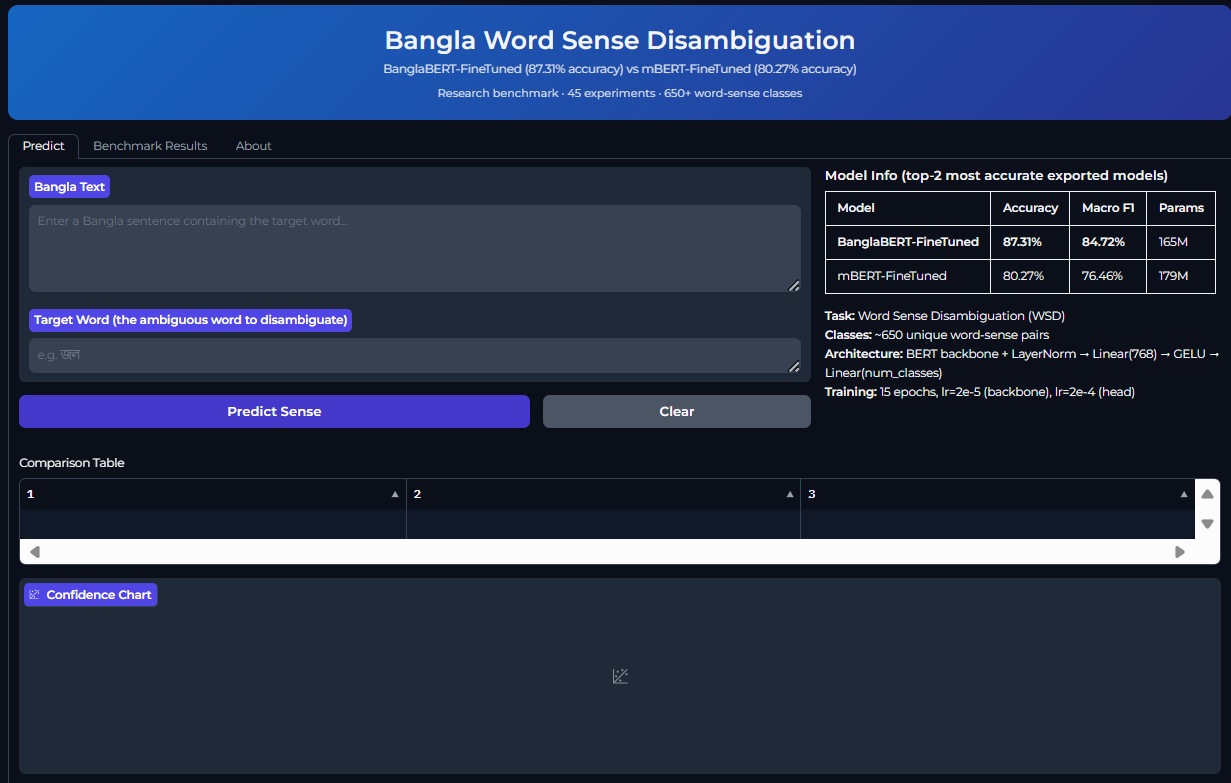
\includegraphics[width=0.92\textwidth]{website_images/new/priliminary.png}
\caption{Step 1 of the worked example: the Predict tab at application start-up, with empty input fields and the Model Info panel listing the two auto-selected fine-tuned models.}
\label{fig:example_step1}
\end{figure}
\begin{figure}[htbp]
\centering
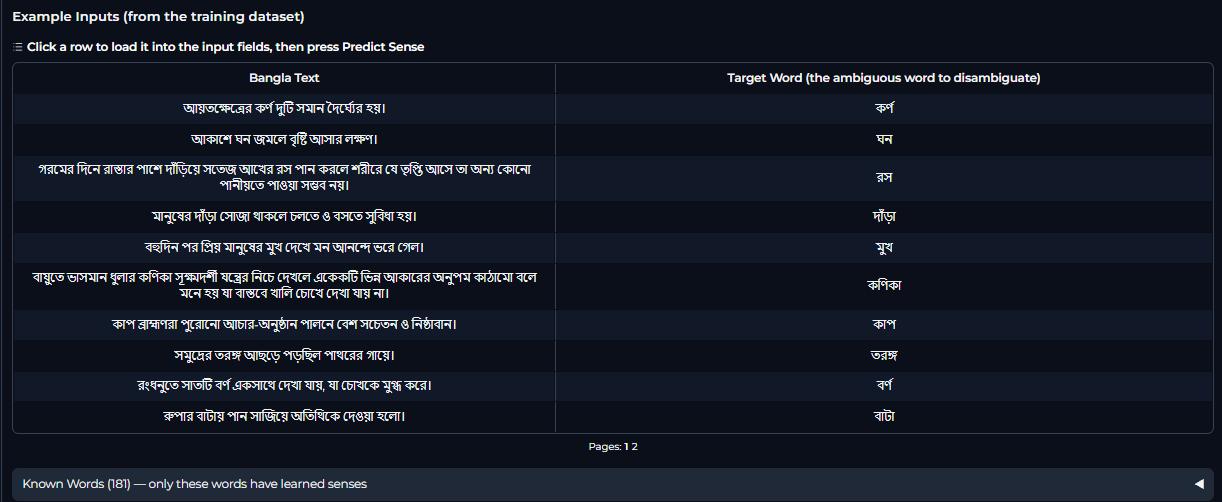
\includegraphics[width=0.92\textwidth]{website_images/new/input_sample.png}
\caption{Step 2 of the worked example: the Example Inputs table, from which clicking a row loads a real corpus sentence and its target word into the input fields.}
\label{fig:example_step2}
\end{figure}
\begin{figure}[htbp]
\centering
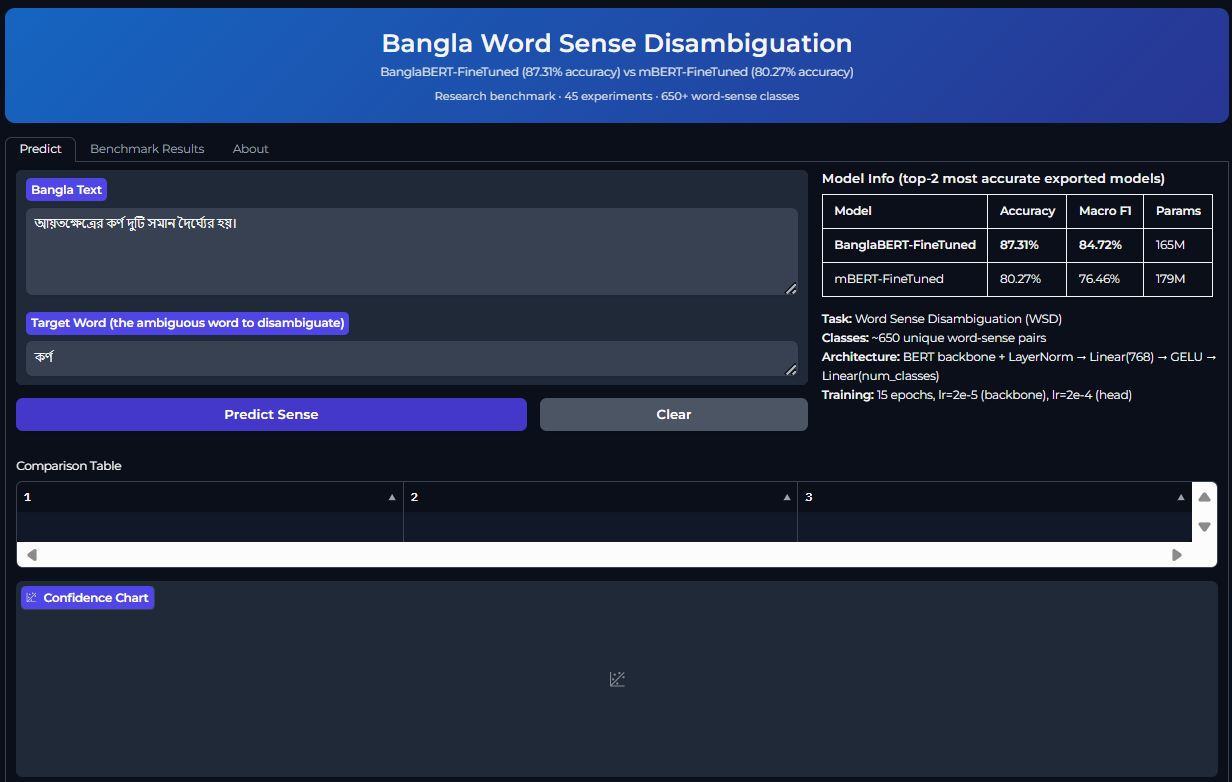
\includegraphics[width=0.92\textwidth]{website_images/new/select_sentence.png}
\caption{Step 3 of the worked example: the sentence \bn{আয়তক্ষেত্রের কর্ণ দুটি সমান দৈর্ঘ্যের হয়।} and target word \bn{কর্ণ} loaded into the input fields, ready for prediction.}
\label{fig:example_step3}
\end{figure}
\begin{figure}[htbp]
\centering
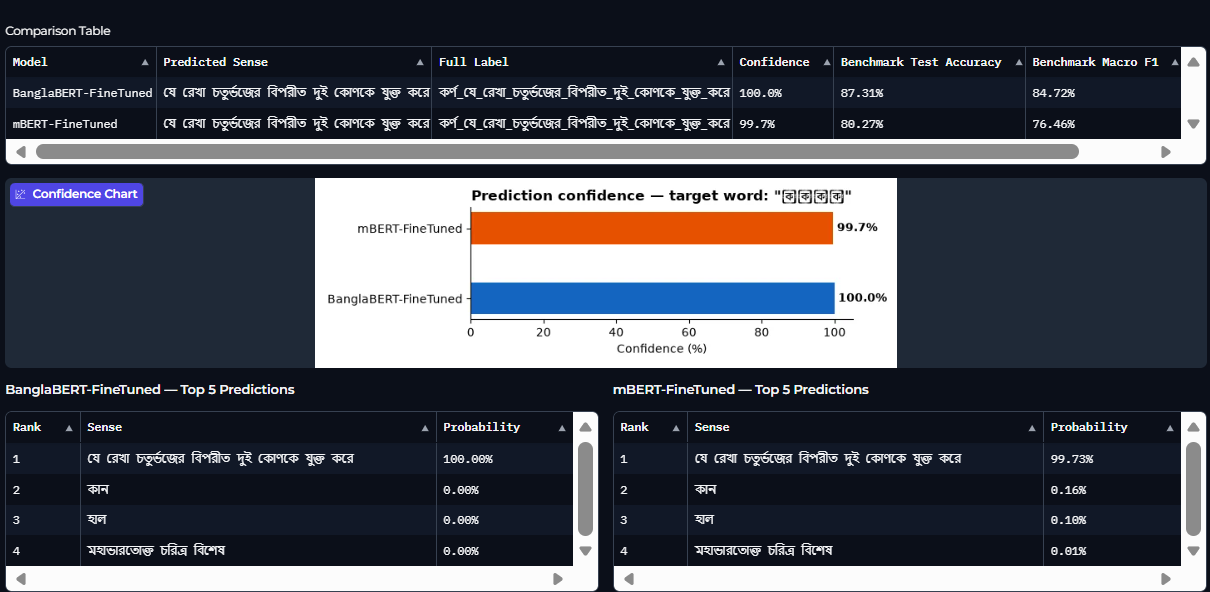
\includegraphics[width=0.92\textwidth]{website_images/new/output.png}
\caption{Step 4 of the worked example: both fine-tuned models predict the geometric \emph{diagonal} sense of \bn{কর্ণ} (100.0\% and 99.7\% confidence), with the three competing senses receiving near-zero probability in the Top-5 tables.}
\label{fig:example_step4}
\end{figure}
\section{Discussion: Mapping Results to Objectives}
{\fontsize{12}{18}\selectfont\normalfont\setstretch{1.5}\justifying\sloppy\emergencystretch=3em
All eight objectives of Section 1.3 were met. The annotation platform (Objective 1) produced a 7,409-sentence, 181-word corpus (Objective 2) with quantified reliability (\(\kappa = 0.836, 0.874\)). The word-specific label re-engineering (Objective 3) yielded 657 non-colliding classes. The twenty-six-experiment embedding/classifier grid and three-backbone fine-tuning stage (Objectives 4-5) were evaluated on a shared metric suite under both global and target-word-constrained inference (Objective 6). Confusion-matrix error analysis (Objective 7) established that over 99\% of the strongest models' residual errors are within-word confusions between semantically adjacent, low-resource sense pairs. The two strongest fine-tuned models were deployed in a self-updating demo (Objective 8). The central empirical findings, that Bangla-specific pretraining (BanglaBERT) outperforms general-purpose multilingual pretraining (mBERT) by 5-7 points once both are fine-tuned; that frozen, target-aware XLM-R embeddings with a linear classifier come within half a point of the fine-tuned leader at a fraction of the cost; and that the same XLM-R backbone fails to fine-tune at all under the shared recipe, directly answer the methodological-narrowness deficiency (Section 1.2) that motivated this thesis: the choice of modelling approach and pretrained backbone measurably matters, and neither can be assumed without a controlled benchmark of the kind conducted here.\par

}
\section{Conclusion}
{\fontsize{12}{18}\selectfont\normalfont\setstretch{1.5}\justifying\sloppy\emergencystretch=3em
This chapter reported Cohen's Kappa reliability results confirming the corpus is trustworthy; a twenty-nine-experiment benchmark in which fine-tuned BanglaBERT (86.82\% accuracy, 85.00\% macro F1) leads, with frozen XLM-R embeddings plus logistic regression close behind at 86.37\% and the best lexical baseline (TF-IDF + Linear SVM) at 64.89\%; a documented XLM-R fine-tuning failure that persists even after the tokenizer, label-space, and gradient-flow hypotheses were each tested and eliminated; confusion-matrix error analysis showing that over 99\% of the strong models' residual errors are within-word confusions between low-resource, semantically adjacent sense pairs; a global-versus-constrained evaluation quantifying how much of each model's error mass is cross-word; and a live demo application that automatically serves the two strongest models. Chapter 5 next considers the ethical, legal, societal, and environmental implications of this work.\par

}

\chapter{Societal, Health, Environment, Safety, Ethical, Legal and Cultural Issues}

\section{Intellectual Property Considerations}
{\fontsize{12}{18}\selectfont\normalfont\setstretch{1.5}\justifying\sloppy\emergencystretch=3em
This thesis produces three original artefacts: the annotation platform source code, the 7,409-sentence annotated corpus, and the trained model checkpoints. The corpus is compiled from example sentences drawn from openly available Bangla reference material and original annotator-composed examples rather than copyrighted literary excerpts, and no personally identifiable third-party content is embedded in it. The platform and benchmark code depend exclusively on permissively licensed open-source software (PHP, MySQL, Python, PyTorch, HuggingFace Transformers, scikit-learn, Gradio), and the three pretrained backbones fine-tuned in this work, multilingual BERT, BanglaBERT, and XLM-RoBERTa, are each released by their original authors under permissive licenses (Apache 2.0 / MIT) that permit fine-tuning and redistribution of derived checkpoints with attribution. No component of this thesis is intended for patent filing; its contribution is an openly reusable dataset, codebase, and benchmark result, and full attribution to the five prior Bangla WSD studies reviewed in Chapter 2 is maintained throughout via citation.\par

}
\section{Ethical Considerations}
{\fontsize{12}{18}\selectfont\normalfont\setstretch{1.5}\justifying\sloppy\emergencystretch=3em
The corpus was produced by two human annotators who gave informed consent, were compensated with a token honorarium (Table 1.1), and were free to skip any sentence they could not confidently label. No personal, sensitive, or identifying information about the annotators or any third party is stored in the corpus; only the annotated sentence, the target word, and the selected sense are retained. Randomizing the order in which candidate senses are presented (Section 3.3) was a deliberate ethical and methodological choice to prevent positional bias from systematically favouring whichever sense a careless annotator clicks first. Because several of the 657 classes are supported by as few as three training examples, the resulting models are less reliable on rare senses (Section 4.6); this limitation is disclosed explicitly rather than presented as uniform accuracy across all senses, so that any downstream application built on this work is not misled about where its predictions are least trustworthy.\par

}
\section{Safety Considerations}
{\fontsize{12}{18}\selectfont\normalfont\setstretch{1.5}\justifying\sloppy\emergencystretch=3em
This is a software-only project with no physical hardware, and it poses no direct physical safety risk. The main safety-adjacent concern is over-reliance on an automated sense prediction in a context where an incorrect sense could cause real harm, for example a mistranslated medical or legal sentence. The live demo application mitigates this by always reporting a confidence score and by explicitly warning when a target word lies outside the 179 words the models were trained on, rather than returning a silent, potentially wrong, guess.\par

}
\section{Legal Considerations}
{\fontsize{12}{18}\selectfont\normalfont\setstretch{1.5}\justifying\sloppy\emergencystretch=3em
The project complies with the licensing terms of every third-party component used: the PHP, MySQL, and Python ecosystems are used under their respective open-source licenses, and the pretrained transformer checkpoints are used and fine-tuned within the terms of their publishers' licenses. No proprietary or access-restricted dataset is used; dataset\_updated.xlsx was compiled specifically for this thesis. Because the annotators are identifiable individuals, their names are referenced only by first name and only within the local project records; no data protection regulation applicable in Bangladesh is violated by this scope.\par

}
\section{Impact of the Project on Societal, Health, and Cultural Issues}
{\fontsize{12}{18}\selectfont\normalfont\setstretch{1.5}\justifying\sloppy\emergencystretch=3em

\subsection{Societal Impact}

As discussed in Section 1.9, a reliable Bangla WSD component can improve machine translation, search, and conversational agents for more than 230 million Bangla speakers. That supports digital inclusion for a language that remains under-served by NLP tooling relative to its number of speakers.\par


\subsection{Health Impact}

The project has no direct health impact; the corpus and models contain no medical content beyond incidental example sentences, and no clinical claim is made or implied.\par


\subsection{Cultural Impact}

The corpus preserves genuine Bangla lexical richness, capturing senses of words such as \bn{জল} and \bn{বর্ণ} (Section 1.1) that are often absent or incomplete in existing machine-readable Bangla resources (Section 2.8). Publishing this resource, together with its human-validated reliability statistic, contributes to the documentation of Bangla as a digitally represented language rather than displacing or homogenising it.\par

}
\section{Impact of the Project on the Environment and Sustainability}
{\fontsize{12}{18}\selectfont\normalfont\setstretch{1.5}\justifying\sloppy\emergencystretch=3em

\subsection{Environmental Impact}

The only energy-intensive component of this project is transformer fine-tuning: three backbones, each trained for up to 15 epochs, on a single Tesla T4 GPU. This is modest by contemporary NLP standards; the entire fine-tuning stage completed within tens of GPU-hours rather than the GPU-days or GPU-months associated with pretraining a language model from scratch, since only fine-tuning, not pretraining, was performed.\par


\subsection{Sustainability Impact}

Using Kaggle's free-tier GPU allocation (Section 1.5) avoided the embodied environmental cost of manufacturing new hardware for a project of this scale, and reusing existing pretrained backbones (Section 2.6) avoided the far larger compute cost of pretraining from scratch.\par


\subsection{Waste Reduction}

All experiment artefacts, including cached embeddings, trained model checkpoints, and results tables, are written once and reused across the twenty-nine experiments (Section 3.8), which cuts redundant computation; nothing is recomputed per run. The failed XLM-R-FineTuned checkpoints (Section 4.5.1) were kept, since the negative result is itself a reusable research artefact documented in this thesis.\par

}

\chapter{Addressing Complex Engineering Problems and Activities}

\section{Introduction}
{\fontsize{12}{18}\selectfont\normalfont\setstretch{1.5}\justifying\sloppy\emergencystretch=3em
This chapter maps this thesis onto the Complex Engineering Problem (CEP) and Complex Engineering Activity (CEA) attributes used by the Washington Accord / Board of Accreditation for Engineering and Technical Education (BAB) framework for engineering-programme accreditation, to show that the work required knowledge, judgement, and activity beyond routine application of a known procedure.\par

}
\section{Complex Engineering Problems Associated with the Thesis}
{\fontsize{12}{18}\selectfont\normalfont\setstretch{1.5}\justifying\sloppy\emergencystretch=3em
Table 6.1 maps each CEP attribute to the specific aspect of this thesis that satisfies it.\par

}
\begin{table}[htbp]
\caption{Complex Engineering Problem (CEP) attributes.}
\label{tab:auto19}
\centering
{\fontsize{10}{14}\selectfont
\begin{tabular}{@{}p{4.20cm} p{10.50cm}@{}}
\toprule
\textbf{Attribute} & \textbf{How This Thesis Satisfies It} \\
\midrule
P1: Depth of engineering knowledge & Requires integrated knowledge of statistical NLP, deep sequence modelling, transformer architectures, database/web-application design, and inferential statistics (Cohen's Kappa), none sufficient alone. \\
\addlinespace[3pt]
P2: Conflicting requirements & Annotation quality versus annotation speed; model accuracy versus inference latency and model size (Table 4.5); and a shared training recipe (fair comparison) versus per-backbone tuning (potentially higher accuracy). \\
\addlinespace[3pt]
P3: Depth of analysis required & Diagnosing the XLM-R fine-tuning failure (Section 4.5.1) required inspecting training-loss trajectories and ROC-AUC across 5 independent runs before concluding it was a genuine backbone-specific phenomenon rather than a bug. \\
\addlinespace[3pt]
P4: Familiarity of issues & No prior Bangla WSD study combined an annotation platform, a reliability check, and a transformer benchmark (Section 1.6); the interfaces between these parts had no established precedent to follow. \\
\addlinespace[3pt]
P5: Extent of applicable codes & Constrained by dataset licensing, open-source software licenses (Section 5.4), and research-ethics norms for human annotation (Section 5.2). \\
\addlinespace[3pt]
P6: Extent of stakeholder involvement & Stakeholders include the two human annotators, the thesis supervisor, and prospective downstream users of the corpus and demo application, each with different priorities (labelling burden, methodological rigour, usability). \\
\addlinespace[3pt]
P7: Interdependence & The pipeline is a strict dependency chain: annotation platform to reliability check to label engineering to embedding/classifier grid to transformer fine-tuning to demo deployment (Section 3.1); a defect early in the chain invalidates every downstream stage. \\
\addlinespace[3pt]
\bottomrule
\end{tabular}}
\end{table}
{\fontsize{12}{18}\selectfont\normalfont\setstretch{1.5}\justifying\sloppy\emergencystretch=3em
}
\section{Complex Engineering Activities Associated with the Thesis}
{\fontsize{12}{18}\selectfont\normalfont\setstretch{1.5}\justifying\sloppy\emergencystretch=3em
Table 6.2 maps each CEA attribute similarly.\par

}
\begin{table}[htbp]
\caption{Complex Engineering Activity (CEA) attributes.}
\label{tab:auto20}
\centering
{\fontsize{10}{14}\selectfont
\begin{tabular}{@{}p{4.20cm} p{10.50cm}@{}}
\toprule
\textbf{Attribute} & \textbf{How This Thesis Satisfies It} \\
\midrule
A1: Range of resources & PHP/MySQL web stack, Python/PyTorch/HuggingFace ML stack, a cloud GPU, human annotators, and pretrained multilingual and Bangla-specific language models. \\
\addlinespace[3pt]
A2: Level of interaction & The annotation platform, the benchmark pipeline, and the live demo application interact through shared artefacts (the exported corpus, the label encoder, results.csv), each consumed by a downstream component built independently. \\
\addlinespace[3pt]
A3: Innovation & The word-specific label re-engineering, the target-word-constrained evaluation protocol, and the automatic top-2 model-selection logic in the demo application are original design decisions not found in the reviewed prior work (Chapter 2). \\
\addlinespace[3pt]
A4: Consequences for society and environment & Positive: improved Bangla NLP infrastructure (Section 5.5.1). Negative risk: over-reliance on automated sense prediction in high-stakes translation, mitigated by confidence reporting (Section 5.3). \\
\addlinespace[3pt]
A5: Familiarity & Extends familiar techniques (Naive Bayes, LSTM/GRU, BERT fine-tuning) to an unfamiliar combination and target language, requiring adaptation rather than routine reuse (Section 1.6). \\
\addlinespace[3pt]
\bottomrule
\end{tabular}}
\end{table}
{\fontsize{12}{18}\selectfont\normalfont\setstretch{1.5}\justifying\sloppy\emergencystretch=3em
}
\section{Conclusion}
{\fontsize{12}{18}\selectfont\normalfont\setstretch{1.5}\justifying\sloppy\emergencystretch=3em
This thesis satisfies all seven CEP attributes and all five CEA attributes of the accreditation framework: it required depth of knowledge spanning multiple sub-disciplines, resolved conflicting requirements between annotation quality, model accuracy, and deployment cost, required non-routine analysis to diagnose the XLM-R failure, addressed a problem with no direct precedent in prior Bangla WSD work, and produced original design contributions (Chapter 2, Section 2.10) rather than a routine application of an existing recipe.\par

}

\chapter{Conclusions}

\section{Summary}
{\fontsize{12}{18}\selectfont\normalfont\setstretch{1.5}\justifying\sloppy\emergencystretch=3em
This thesis set out to address three deficiencies in Bangla Word Sense Disambiguation research: the absence of a large, publicly verifiable, reliability-checked benchmark corpus; the absence of a quantified inter-annotator reliability check in any prior study; and the absence of a controlled comparison spanning classical machine learning through transformer fine-tuning. A PHP/MySQL annotation platform, built specifically for this work, was used to construct a 7,409-sentence corpus across 181 target words, with reliability quantified at \(\kappa = 0.836\) and \(0.874\) ("almost perfect", Landis and Koch). A word-specific label re-engineering eliminated cross-word sense collisions and left 657 non-colliding classes across 179 words after preprocessing. A controlled, twenty-nine-experiment benchmark then compared six embeddings (three of them pretrained static or frozen transformer representations with target-aware pooling), three classical learners, four recurrent architectures, and three fully fine-tuned transformers under one fixed stratified split and one shared metric suite, with every configuration additionally scored under target-word-constrained inference. Fine-tuned BanglaBERT achieved the best result, 86.82\% accuracy and 85.00\% macro F1, outperforming fine-tuned multilingual BERT by 7.2 macro-F1 points, controlled evidence that Bangla-specific pretraining beats general-purpose multilingual pretraining on this task, while frozen XLM-RoBERTa target-span embeddings with plain logistic regression came within half an accuracy point of the fine-tuned leader at a small fraction of its training cost. Fine-tuning XLM-RoBERTa itself under the identical recipe failed to converge (0.09\% accuracy), a negative result documented with tokenizer, label-space, gradient-flow, training-curve, and ROC-AUC evidence. The two strongest fine-tuned models were deployed in a self-updating Gradio application. Taken together, this thesis contributes a reusable, human-validated Bangla WSD resource and what appears to be the first systematic comparison of classical, deep-learning, and transformer-based approaches to Bangla word sense disambiguation under a single, controlled experimental protocol; none of the studies reviewed in Chapter 2 reports one.\par

}
\section{Limitations}
{\fontsize{12}{18}\selectfont\normalfont\setstretch{1.5}\justifying\sloppy\emergencystretch=3em
Several limitations, most already flagged where they first arise, are consolidated here for clarity.\par

\begin{enumerate}[leftmargin=*, itemsep=4pt]
  \item All twenty-nine experiments use one fixed stratified split (seed 42), so no empirical estimate of split-to-split variance is reported; the split indices are persisted for exact reproducibility, but repeating the benchmark across multiple independent splits remains future work (Section 1.4).
  \item XLM-RoBERTa fine-tuning fails to converge under the shared training recipe even after the [TGT] markers are registered as atomic special tokens and label mapping and gradient flow are verified (Section 4.5.1); whether a backbone-specific learning rate or warm-up schedule would allow it to succeed remains open.
  \item The fitted TF-IDF, Word2Vec, and fastText artefacts were not exported alongside the trained classifiers, so only the fine-tuned transformers are runnable in the live demo application.
  \item Several of the 657 classes are supported by as few as seven examples in total (about five in training), and Section 4.6 shows that under-represented, semantically adjacent senses of the same target word account for over 99\% of the strongest models' residual errors.
  \item The corpus follows a target-word (lexical-sample) formulation across 179 words rather than an all-words formulation, consistent with the scope defined in Section 1.4 but not directly comparable to all-words WSD benchmarks in other languages.
  \item Annotation reliability was measured between two annotators; a larger annotator pool would allow a more robust reliability estimate and broader sense coverage per word.
\end{enumerate}
}
\section{Recommendations for Future Works}
{\fontsize{12}{18}\selectfont\normalfont\setstretch{1.5}\justifying\sloppy\emergencystretch=3em
Building on the findings and limitations above, the following directions are recommended.\par

\begin{enumerate}[leftmargin=*, itemsep=4pt]
  \item Diagnose and repair XLM-RoBERTa fine-tuning, for example via a lower or layer-wise-decayed learning rate, longer warm-up, or gradient-checkpointed longer training, to determine whether its failure is recoverable under this task and label space.
  \item Export the fitted TF-IDF, Word2Vec, and fastText artefacts so that all twenty-nine, not only the fine-tuned, configurations are runnable in the live demo application; the near-parity of frozen XLM-R + Logistic Regression with the fine-tuned leader makes a lightweight frozen-embedding deployment particularly attractive.
  \item Repeat the benchmark across multiple independent stratified splits to attach confidence intervals to the single-split results reported here.
  \item Apply few-shot or meta-learning approaches to the under-represented senses identified in Section 4.6 as the dominant error source.
  \item Extend the corpus beyond 181 target words and beyond two annotators, with a second Cohen's-Kappa round to confirm reliability holds as the corpus and annotator pool grow.
  \item Extend the target-word (lexical-sample) formulation of this thesis toward an all-words Bangla WSD setting, contingent on improved Bangla WordNet coverage (Section 2.8).
  \item Explore parameter-efficient fine-tuning (LoRA, adapters) as a lighter-weight alternative to full fine-tuning, potentially narrowing the accuracy gap for backbones such as XLM-R while reducing the memory footprint reported in Table 4.5.
\end{enumerate}
This thesis demonstrates that a human-validated, reliability-checked Bangla WSD corpus, combined with a controlled benchmark spanning classical machine learning through transformer fine-tuning, can identify which approach performs best (fine-tuned, Bangla-specific pretraining) and where such approaches fail unexpectedly (XLM-R under the shared recipe); a narrower, single-model study could not have produced either finding.\par

}

\begin{thebibliography}{99}

\bibitem{ide1998wsd}
N.~Ide and J.~V\'eronis, ``Word Sense Disambiguation: The State of the Art,''
\textit{Computational Linguistics}, vol.~24, no.~1, pp.~1--40, 1998.

\bibitem{navigli2009wsd}
R.~Navigli, ``Word Sense Disambiguation: A Survey,''
\textit{ACM Computing Surveys}, vol.~41, no.~2, pp.~1--69, 2009.

\bibitem{mikolov2013word2vec}
T.~Mikolov, K.~Chen, G.~Corrado, and J.~Dean, ``Efficient Estimation of Word
Representations in Vector Space,'' arXiv:1301.3781, 2013.

\bibitem{bojanowski2017fasttext}
P.~Bojanowski, E.~Grave, A.~Joulin, and T.~Mikolov, ``Enriching Word Vectors
with Subword Information,'' \textit{Transactions of the Association for
Computational Linguistics}, vol.~5, pp.~135--146, 2017.

\bibitem{devlin2019bert}
J.~Devlin, M.-W.~Chang, K.~Lee, and K.~Toutanova, ``BERT: Pre-training of Deep
Bidirectional Transformers for Language Understanding,'' in \textit{Proc.\
NAACL-HLT}, 2019.

\bibitem{conneau2020xlmr}
A.~Conneau et al., ``Unsupervised Cross-Lingual Representation Learning at
Scale,'' in \textit{Proc.\ ACL}, 2020.

\bibitem{bhattacharjee2022banglabert}
A.~Bhattacharjee et al., ``BanglaBERT: Language Model Pretraining and
Benchmarks for Low-Resource Language Understanding Evaluation in Bangla,''
in \textit{Findings of NAACL}, 2022.

\bibitem{cohen1960kappa}
J.~Cohen, ``A Coefficient of Agreement for Nominal Scales,''
\textit{Educational and Psychological Measurement}, vol.~20, no.~1,
pp.~37--46, 1960.

\bibitem{landis1977kappa}
J.~R. Landis and G.~G. Koch, ``The Measurement of Observer Agreement for
Categorical Data,'' \textit{Biometrics}, vol.~33, no.~1, pp.~159--174, 1977.

\bibitem{palsaha2019}
A.~R. Pal and D.~Saha, ``Word Sense Disambiguation in Bengali Language Using
Unsupervised Methodology with Modifications,'' \textit{S\=adhan\=a},
vol.~44, no.~168, pp.~1--13, 2019.

\bibitem{sahamoumittra2019}
P.~K. Saha, A.~D. Mou, and T.~Mittra, ``A Bangla Word Sense Disambiguation
Technique Using Minimum Edit Distance Algorithm and Cosine Distance,'' in
\textit{Proc.\ IEEE}, 2019.

\bibitem{dasdawn2023}
D.~Das Dawn, A.~Khan, S.~H. Shaikh, and R.~K. Pal, ``A Dataset for Evaluating
Bengali Word Sense Disambiguation Techniques,'' \textit{Journal of Ambient
Intelligence and Humanized Computing}, vol.~14, pp.~4057--4086, 2023.

\bibitem{kaysarkhan2018}
M.~S. Kaysar and M.~I. Khan, ``Word Sense Disambiguation for Bangla Words
Using Apriori Algorithm,'' in \textit{Proc.\ ICRAMPS}, 2018.

\bibitem{nazah2017}
S.~Nazah, M.~M. Hoque, and M.~R. Hossain, ``Word Sense Disambiguation of
Bangla Sentences Using Statistical Approach,'' in \textit{Proc.\ IEEE 3rd
Int.\ Conf.\ Electrical Information and Communication Technology (EICT)},
2017.

\end{thebibliography}

%============================================================
%  APPENDIX A  –  Dataset Sample
%============================================================
\newpage
\thispagestyle{plain}
\addcontentsline{toc}{chapter}{Appendix A: Dataset Sample}
% Appendix tables are numbered A.1, A.2, ... rather than continuing
% the chapter-based Chapter.Sequence numbering of the main body.
\renewcommand{\thetable}{A.\arabic{table}}
\setcounter{table}{0}

\begin{center}
{\fontsize{16}{24}\selectfont\bfseries Appendix A\\[6pt]Dataset Sample}
\end{center}

\twoblank

{\fontsize{12}{18}\selectfont\normalfont\setstretch{1.5}\justifying\sloppy\emergencystretch=3em
This appendix reproduces a verbatim sample of the corpus file dataset\_updated.xlsx described in Section 3.2, so that the structure of the resource contributed by this thesis can be inspected directly. The full file contains 7,409 rows, each carrying five fields: word\_id (numeric identifier of the polysemous target word), target\_word (its surface form), sense\_id (the index of the sense assigned to that occurrence, unique only within its target word), sense\_gloss (a short Bangla gloss defining the sense), and text (the complete example sentence in which the target word is used in that sense). Table A.1 lists one example sentence per sense for six representative target words, chosen because each is discussed in the body of the thesis: \bn{বর্ণ} and \bn{হাত} are the cross-word label-collision examples of Sections 1.2 and 3.5, \bn{রূপ} is the sentiment-bearing example of Section 1.9, \bn{ধারা} is the most heavily annotated word in the corpus (Section 3.2), and \bn{মুখ} and \bn{কাল} illustrate the typical four-way sense inventories that dominate the corpus (Figure 3.2b). All sentences appear exactly as stored in the file. The complete dataset is available from the author on request.\par

}
{\fontsize{10}{14}\selectfont
\begin{longtable}{@{}p{2.3cm} p{1.1cm} p{3.0cm} p{7.4cm}@{}}
\caption{Verbatim sample of the Bangla WSD corpus file dataset\_updated.xlsx: one example sentence per sense for six representative target words.}
\label{tab:appendix_dataset_sample}\\
\toprule
\textbf{Target Word (word\_id)} & \textbf{Sense ID} & \textbf{Sense Gloss} & \textbf{Example Sentence (text)} \\
\midrule
\endfirsthead
\multicolumn{4}{@{}l}{\itshape Table \thetable{} (continued)}\\[3pt]
\toprule
\textbf{Target Word (word\_id)} & \textbf{Sense ID} & \textbf{Sense Gloss} & \textbf{Example Sentence (text)} \\
\midrule
\endhead
\midrule
\multicolumn{4}{r@{}}{\itshape continued on next page}\\
\endfoot
\bottomrule
\endlastfoot
\bn{বর্ণ} (3) & 1 & \bn{রঙ} & \bn{পাকা আমের হলদে বর্ণ দেখলে মনে লালসা জাগে।} \\
\addlinespace[3pt]
 & 2 & \bn{হিন্দুসমাজের বিভাগ} & \bn{আধুনিক ভারতের সংবিধানে বর্ণ ভিত্তিক বৈষম্যকে নিষিদ্ধ করা হয়েছে।} \\
\addlinespace[3pt]
 & 3 & \bn{অক্ষর} & \bn{বইয়ের মলাটে বড় হরফে লেখা বর্ণগুলো আলোতে চকচক করছিল।} \\
\midrule
\bn{মুখ} (13) & 1 & \bn{আনন} & \bn{অসুস্থ লোকটির মুখে বিষণ্নতার ছাপ স্পষ্ট।} \\
\addlinespace[3pt]
 & 2 & \bn{ছিদ্র} & \bn{কামানের মুখ দিয়ে গোলা বের হয়।} \\
\addlinespace[3pt]
 & 3 & \bn{অগ্রভাগ} & \bn{হাতুড়ির মুখ দিয়ে পেরেক ঠোকা হয়।} \\
\addlinespace[3pt]
 & 4 & \bn{দিক/অভিমুখ} & \bn{নদীর মুখ উত্তর দিকে বলে সেদিকে স্রোত বেশি থাকে।} \\
\midrule
\bn{কাল} (29) & 1 & \bn{ঋতু} & \bn{শীতকাল কুয়াশার মৌসুম।} \\
\addlinespace[3pt]
 & 2 & \bn{আগামী দিন} & \bn{তুমি কাল কোথায় যাবে?} \\
\addlinespace[3pt]
 & 3 & \bn{অতিশয় ঠাণ্ডা} & \bn{কাল ঠান্ডায় পাইপের পানি জমে গেছে।} \\
\addlinespace[3pt]
 & 4 & \bn{কৃষ্ণবর্ণ} & \bn{কাল মেঘে আকাশ ঢেকে গেছে।} \\
\midrule
\bn{ধারা} (105) & 1 & \bn{জলপ্রবাহ} & \bn{ঝরনার ধারা পাথর ক্ষয় করে গভীর খাল তৈরি করেছে।} \\
\addlinespace[3pt]
 & 2 & \bn{আইনগত ধারা} & \bn{আসামিকে দণ্ডবিধির ৩০২ ধারায় অভিযুক্ত করা হয়েছে।} \\
\addlinespace[3pt]
 & 3 & \bn{ধারাবাহিকতা} & \bn{বিজয়ের এই ধারা বজায় থাকলে দলটি শিরোপা জিততে পারবে।} \\
\addlinespace[3pt]
 & 4 & \bn{রীতি} & \bn{বাংলার লোকসংস্কৃতিতে নববর্ষ উদযাপনের নিজস্ব ধারা আছে।} \\
\midrule
\bn{রূপ} (114) & 1 & \bn{আকৃতি} & \bn{মোম গলে নতুন রূপ ধারণ করল।} \\
\addlinespace[3pt]
 & 2 & \bn{সৌন্দর্য} & \bn{মা মেয়ের রূপ দেখে গর্বিত হলেন।} \\
\addlinespace[3pt]
 & 3 & \bn{অবস্থা} & \bn{দেশের বর্তমান রূপ দেখে অনেকেই হতাশ।} \\
\addlinespace[3pt]
 & 4 & \bn{প্রকাশভঙ্গি} & \bn{শোকের রূপ সবার কাছে এক নয়।} \\
\midrule
\bn{হাত} (150) & 1 & \bn{শরীরের অঙ্গ} & \bn{শীতের সকালে হাত দুটো ঠান্ডায় কাঁপছিল।} \\
\addlinespace[3pt]
 & 2 & \bn{সাহায্য} & \bn{একে অপরকে হাত না দিলে সমাজ এগোয় না।} \\
\addlinespace[3pt]
 & 3 & \bn{দক্ষতা} & \bn{এই কাজে তার হাত অনেক পাকা।} \\
\addlinespace[3pt]
 & 4 & \bn{পরিমাপ} & \bn{এই কাপড়টি চার হাত লম্বা।} \\
\end{longtable}}

\end{document}